% \documentclass[12pt,a4paper,twoside]{scrbook}
\documentclass{hepthesis}

\usepackage{setspace}
\onehalfspacing

\usepackage{multicol}
\usepackage{paralist}
\usepackage{amsfonts}
\usepackage{multirow}
\usepackage{listings}
\usepackage{graphicx}
\usepackage{ccicons}
\usepackage{url}
\usepackage{color} 
\usepackage[colorlinks=true]{hyperref}

\newcommand{\ra}[1]{\renewcommand{\arraystretch}{#1}}
\newcommand{\hs}{\hspace{0.1in}}

\makeatletter
\@ifpackageloaded{hyperref}{%
\hypersetup{%
pdftitle = {Interlinking Personal Semantic Data},
pdfkeywords = {Semantic Desktop, Personal Information Management},
pdfauthor = {Laura Dragan}
}
}{}
\makeatother

\lstdefinelanguage{turtle}{
morekeywords={@prefix, a}, 
sensitive=false, 
morecomment=[l]{\#}, 
morestring=[b]",
}

\lstdefinelanguage{htmlrdfa}{
  keywords={DOCTYPE, html, head, title, body, about, meta, content, property, rel, href, a}, 
  keywordstyle=\color{blue}\bfseries,
  sensitive=false, 
  morestring=[b]',
  morestring=[b]",
}

\lstdefinelanguage{js}{
  keywords={typeof, new, true, false, catch, function, return, null, catch, switch, var, if, in, while, do, else, case, break},
  keywordstyle=\color{blue}\bfseries,
  ndkeywords={class, export, boolean, throw, implements, import, this},
  ndkeywordstyle=\color{darkgray}\bfseries,
  identifierstyle=\color{black},
  sensitive=false,
  comment=[l]{//},
  morecomment=[s]{/*}{*/},
  commentstyle=\color{purple}\ttfamily,
  stringstyle=\color{black}\ttfamily,
  morestring=[b]',
  morestring=[b]"
}

\lstset{
  captionpos=b, 
  extendedchars=true,
  basicstyle=\scriptsize \sffamily, 
  stringstyle=\bfseries,
  frame=single,
  frameround=tttt,
  showstringspaces=false,
  breaklines=true,
}

\renewcommand{\lstlistlistingname}{List of Listings}

\title{Interlinking Personal Semantic Data}
\author{Laura C\u{a}ta\u{a}lina Dr\u{a}gan}

\begin{document}

\begin{frontmatter}
 \thispagestyle{empty}

\begin{figure}
\centering
  
\includegraphics[width=0.8\textwidth]{frontmatter/img/nuig_logo.jpg}
\end{figure}

\vspace*{0.5cm}

\begin{center}
{\huge Interlinking Personal Semantic Data\par} 
{\Large on the Semantic Desktop and the Web of Data\par}
\vspace*{1cm}
\end{center}

\begin{center}
\textbf{Laura C\u{a}t\u{a}lina Dr\u{a}gan}
\end{center}

\begin{center}
\vspace{2cm}

{\normalsize Submitted in fulfilment of the requirements for the degree of\\
Doctor of Philosophy\\ \par}

\vspace{2cm}

SUPERVISOR:\\
\textbf{Dr. Siegfried Handschuh}\\

\vspace{0.5cm}

\begin{multicols}{2}
\begin{center}
INTERNAL EXAMINER:\\
\textbf{Prof. Dr. Stefan Decker}\\
\vspace{5cm}
EXTERNAL EXAMINER:\\
\textbf{Prof. Dr. Enrico Motta}\\
\end{center}
\end{multicols}

\vspace{1cm} \hrule \vspace{0.4cm} Digital Enterprise Research Institute (DERI),\\ National University of Ireland, Galway\\
September 2012
\end{center}


\vspace*{1cm} 
\vfill
\begin{small}
The work reported in this thesis was supported by Science Foundation Ireland (SFI) under the DERI-L\'{i}on project (SFI/02/CE1/I131) and the DERI-L\'{i}on--II project (SFI/08/CE/I1380) and by the European Union 6th Framework under the NEPOMUK IP (FP6-027705) project.
\end{small}
\bigskip
\begin{center}
\hrule
\bigskip
\ccby~Laura Dr\u{a}gan, 2012
\end{center}

\cleardoublepage
\section*{Abstract}

With the goal of improved Personal Information Management, the Semantic Desktop emerged as a solution to the problem of data fragmentation and disconnection on the desktop. It provides a framework based on Semantic Web standards and technologies, for interlinking desktop information. Interlinked data mimics the user's mental model, and as a result it is easier to manage, to find and refind, thus also offering a solution to the information overload problem. The Semantic Desktop overcomes limitations of the conventional desktop by using a common representation for the data, common vocabularies to describe it, and a desktop-central place to store it. Thus, it creates a network of linked desktop data, in a standardised format, accessible to all applications. 
However, having a relatively stable framework for the Semantic Desktop does not end the quest for improved Personal Information Management. 

To users, the Semantic Desktop framework is a transparent layer, and as such, its benefits must shine through the applications which use it. And so the challenge of designing \emph{good} semantic applications for the Semantic Desktop emerges. Important facets of this challenge include: presenting and visualising data, handling the relations among desktop entities, and incorporating new semantic information into the existing network of connected data. 
A second challenge is generated by the fact that the desktop, even a semantic one, is no longer sufficient for our information needs. The ever growing amount of online data, and the increasing volume of it which is available in structured form, enables further interlinking of personal semantic information with the Web of Data, to the benefit of the user.

In order to address these challenges, we follow the theme of interlinking personal semantic data in two threads through this thesis. First locally, within the Semantic Desktop, interlinking must be supported, and even more so \emph{encouraged} by semantic applications built on top of the framework. We describe the challenges of designing and developing a semantic application for the Semantic Desktop, and present our SemNotes as an example, detailing the design decisions made along the way. The second direction extends to bridging the gap between the Semantic Desktop and the Web of Data, through connecting matching entities from the two spaces. This bridge opens up the possibility of using the rich data from the Web to complement and augment a user's personal information in new and innovative ways. 

\cleardoublepage
\tableofcontents

\listoffigures
\listoftables
\lstlistoflistings
\addcontentsline{toc}{chapter}{List of Listings}

\end{frontmatter}

\begin{mainmatter}
 \part{Prelude}
\label{part:prelude}

\chapter{Introduction}
\label{ch:introduction}

We accumulate massive amounts of information on our computers and other devices, so much that it becomes daunting and sometimes useless because it is impossible to remember it all: emails, appointments, tasks, documents, people, conversations, etc. In traditional desktop architectures this information is created and stored in various applications, each an isolated island of data, with its own storage and its own format, unaware of related and relevant data in other applications. But in our mind this information is not separate, rather everything is connected by implicit links. When we use information we do not work with just one detached slice of it, but we mentally follow connections to other pieces of information from multiple sources. Information is inherently interlinked and used in an integrated fashion.

The Semantic Desktop emerged as a solution to the data fragmentation and disconnection problem. It provides a foundation and a framework based on Semantic Web standards and technologies, for interlinking information on the desktop. Interlinked information is easier to manage and organise, and because it mimics users' mental models, it is easier to find when required, thus also offering a solution to the information overload problem. The Semantic Desktop overcomes limitations of conventional desktops by using a common representation for the data, common vocabularies to describe it, and a central place to store it. It creates a network of linked desktop data, in a standardised format, which is accessible to all applications.

Several implementations of Semantic Desktops exist, with varied function sets and capabilities. NEPOMUK is a project undertaking the task of creating a blueprint for the Semantic Desktop. 
The work presented in this thesis is grounded and built upon the framework provided by Nepomuk-KDE, a branch of the NEPOMUK project. 

The most common use case for the Semantic Desktop is Personal Information Management (PIM). However, having a relatively stable framework for the Semantic Desktop does not bring the search for improved PIM to an end, rather it uncovers a path to a solution. There is plenty of work ahead, exploiting and improving the framework based on experience, research and testing. This thesis focuses on providing new and improved means of creating and maintaining the network of interconnected personal semantic data, on the desktop and beyond.

\section{Problem Statement}
\label{sec:problem}

The Semantic Desktop provides a solid framework for applications and systems to support the use of semantics on the desktop. However, having this framework is not enough, as the success and validation of any framework is reflected in its uptake and use. A key challenge that emerges is how to design and implement good semantic applications that use the infrastructure provided by the Semantic Desktop. This is a very vague and underspecified issue, that we divide into smaller problems for which we provide solutions. Important facets include presenting and visualising data, handling the relations among desktop entities, and incorporating new semantic data into the existing network.

The Semantic Desktop connects information in a network of linked personal data. Adding the, still mostly experimental, social aspect of sharing semantic personal data, and collaborating on it, we get clusters of networks of linked personal data. However, there is already a much larger network of Linked Data on the Web. The openly available Linked Data has grown extensively in recent years, as shown by the successive visual representations of the Linking Open Data cloud\footnote{\url{http://lod-cloud.net} Linking Open Data cloud diagram, by Richard Cyganiak and Anja Jentzsch.}. 
With such a vast network of Linked Data available, but unconnected to the desktop, the next step is to connect these two networks. This task is made easier by the fact that they share the same representation language, yet it is complicated by the different vocabularies used to describe the data, as well as the difference between the open world assumption of the Web versus the closed world assumption of the desktop. Building the bridge between these two domains raises several challenges, from ensuring privacy and security, to finding the best information in the large amount of available data.

\section{Research Questions}
\label{sub:question}

The above challenges are materialised into more precise research questions. At a general level, two questions will be tackled in the following chapters, each of them divided into more detailed sub-questions.

We start from the premise of the existing Semantic Desktop which solves the architectural issues, and gives a stable framework to build upon. However, it does not provide a complete ecosystem able to support the user in some of the more complex tasks. As such, we focus on two complementary directions:

Starting from the desktop environment, we look into:
\begin{description}
 \item[Q 1.] \emph{How to build semantic applications and tools for the Semantic Desktop to provide the best experience for the users, while creating reusable semantic data?}
\end{description}
And then we expand the scope from the desktop to the larger domain of the Web of Data:
\begin{description}
 \item[Q 2.] \emph{How to expand the scope of the Semantic Desktop into the realm of the Web of Data, to benefit the users and enhance their experience?}
\end{description}
We divide these questions into more specific sub-questions, that describe the facets of the issues tackled.

While building on top of the Semantic Desktop, there are additional challenges beside the ones raised by normal application design and development.

\begin{description}
 \item[Q 1.1.] \emph{How to create semantic data that is correct, and maximises the reuse of existing Semantic Desktop data through interlinking?}
\end{description}

Due to the blackboard type of architecture of the Semantic Desktop, applications should not be developed in a vacuum, but rather, they should be aware of other data that is available to them, and also be aware that the data they produce will be accessible to other tools. This raises the dual challenge of making sure the data is represented correctly so that other applications can use it, if they choose to, as well as ensuring the privacy and security of the data created. While is is impossible to say that information created is ever complete, applications must ensure that the data they create contains at least the minimum amount of information as to be usable by others. This requirement depends on the type of data created, but for new resources it includes basic properties such as a label to be used for display. Regarding the correctness of the data created, this requirement refers mainly to the way information is described according to the ontologies used, rather than being correct factually, which is a 
harder task and depends on factors outside the control of the application developers. Correctly described data contributes also to the last point of the question, enabling better discovery and reuse. 

The possibility of reusing vast amounts of existing data raises other challenges, in selecting the right subset of necessary information for maximum benefit, while not overloading the users with it. The selection is complemented by the way the information is shown:

\begin{description}
 \item[Q 1.2.] \emph{How to design the human-computer interaction in an application for the Semantic Desktop?}
\end{description}

The question refers to more than just displaying the information in an interface. Collecting input from the users, and generally supporting the creation of new semantic data is also a challenge. An extra difficulty is added by the heterogeneity of interlinked information available on the desktop, combined with the reduced control of developers over what resources are linked from other tools. 

While it has been demonstrated by several studies that semantic tools are better than non-semantic counterparts \cite{Sauermann2008,Franz2009} in supporting users in PIM tasks, evaluating semantic applications for the Semantic Desktop is still a difficult task to undertake. Therefore, the next question is: 

\begin{description}
 \item[Q 1.3.] \emph{How to correctly evaluate a semantic application?}
\end{description}

The challenge comes from the lack of a standard dataset on which to perform the evaluation. Even if such a dataset existed, due to the fact that the applications on the Semantic Desktop are mainly related to personal information, it is difficult for test participants to use the data provided, as they are not familiar with it. Evaluating PIM tools has been shown to yield more accurate results when the test users are asked to perform their own tasks in their own set-up, rather than attempting to simulate it with artificial tasks and data \cite{Kelly2006}. The reduced number of semantic applications in each area make it difficult to evaluate a new tool against an existing established one, thus leaving the alternative of evaluating against an existing non-semantic application. While possibly re-demonstrating that indeed linked data is more useful, comparing a semantic and non-semantic application requires well-thought metrics, as the semantic features that need to be evaluated have no direct counterparts against 
which to check them.

The second research question refers to connecting the Semantic Desktop to the Web of Data. The large amount of data available on the Web makes it difficult to find relevant information. An important part of connecting the Semantic Desktop to the Web of Data is finding common entities, like people or events, which might appear in both datasets. But entity resolution is hard when the input dataset is very large, and when only limited information is available for discriminating between similar entities. Therefore:

\begin{description}
 \item[Q 2.1.] \emph{How to find instances representing the same real-world thing described by a Semantic Desktop resource?}
\end{description}

Examples include persons, organisations, projects, events, and documents. Since both networks of Linked Data (on the desktop and on the Web) use the same representation, improvements in the graph matching algorithms help, but the two sides are unbalanced and most often use different vocabularies to describe the data.
Reconciling the desktop ontologies with the vocabularies used on the Web of Data requires mapping the ``few'' ontologies in the former category to the seemingly infinite number of vocabularies in the latter. 

\begin{description}
 \item[Q 2.2.] \emph{How to use the Web information which is related to a desktop resource?} 
\end{description}

The answer to the question depends of course on the application that uses the information and the desktop resource, but some points are general: retaining the provenance of each piece of information imported; finding and handling conflicting information and judging trust; deciding if and when should local information be deprecated and replaced with new Web information. 

Furthermore, connecting the Semantic Desktop to the Web of Data does not necessarily imply a unidirectional relation. A reverse link from the Web of Data to the Semantic Desktop should be considered as well. As always when making personal information available online, privacy concerns must be taken into account.

\begin{description}
 \item[Q 2.3.] \emph{How to make desktop data available online safely?}
\end{description}

While accessing desktop information from the Web is technically possible, in principle it goes against the idea of a closed personal Semantic Desktop. The suitable way of making desktop data available online is by publishing it, thus making it part of the Web of Data. 
Publishing information from the desktop is a simple enough task, but privacy issues arise when the data in question is highly interlinked with other private information.

Following the directions given by the two general questions, the approach we use focuses first on interlinking Semantic Desktop data through new semantic applications, and continues with linking the desktop to the Web of Data, through establishing new connections to the outside.


\section{Approaches and Main Contributions}
\label{sec:contribution}

In order to answer the two research questions detailed above, the thesis describes two complementary directions for expanding the network of personal semantic data of the Semantic Desktop: creating connections within the desktop, and externally to the Web. 

The first direction, creating new semantic data inside the Semantic Desktop, including new connections between entities, focuses on enabling the users to do so, through semantic applications. We recognise the need for semantic applications designed specifically for the Semantic Desktop, as the framework provides capabilities above what the conventional tools can support. To demonstrate solutions to the challenges of developing semantic applications mentioned above, we describe the design process and implementation of SemNotes, a semantic note-taking tool. Although a relatively small application, it covers all the phases of the semantic data life-cycle as described in \cite{MoellerPhDThesis2009}, and does so in an unrestricted domain of use. We have written about developing SemNotes in \cite{Dragan2009a} and in more detail in \cite{Dragan2011a}.

The second, external direction of bridging the gap between the Semantic Desktop data and the Web of Data looks at capitalising on the common representation and structure of the data in the two networks. Because the two worlds are rarely disconnected, and a large part of the entities from the desktop appear online as well, we define and implement an algorithm which finds Web aliases for desktop resources. This part of the work initiated from linking publication information \cite{Groza2009} on the desktop and on the Web, and continued with a use case focused on publishing semantic notes as semantic blog posts without losing link annotations \cite{Dragan2010a}. The finalised algorithm and its evaluation are described in \cite{Dragan2011b}. 

To establish the background for the following work, we present a survey of Semantic Desktop systems and applications, which is an extended version of the one published as \cite{Dragan2012}.

\begin{table}
\centering
\ra{1.3}
\begin{tabular}{@{}lc@{\hs}l@{\hs}}
\toprule
Chapter & \phantom{a} & Research questions\\ 
\midrule

 \ref{ch:semnotes} Creating and Interlinking Semantic Data && \textbf{Q 1.1. Q 1.2. Q 1.3.}  \\ 

 \hfill on the Desktop with SemNotes && \\

 \ref{ch:sdwod} Bridging the Gap between the Semantic && \textbf{Q 2.1. Q 2.2.} \\

 \hfill Desktop and the Web of Data && \\

 \ref{ch:semblogging} Transforming Semantic Notes into && \textbf{Q 2.2. Q 2.3.} \\
 
 \hfill Semantic Blog Posts && \\

 \ref{ch:mischelperapps} Additional Extensions and Applications && \textbf{Q 1.1. Q 1.2. Q 2.1. Q 2.2.} \\

\bottomrule
\end{tabular}
\caption{The research questions tackled in each chapter.}
\label{tab:chaptersquestions}
\end{table}

\section{Thesis Outline}
\label{sec:outline}

The remainder of the thesis is structured as follows: 

\subsection*{Part \ref{part:background} --- Foundations}

We begin by setting the foundations for our work. This part is comprised of two chapters. 

\begin{description}
\item[Chapter \ref{ch:background}] describes the terminology and introduces some of the related work about the Semantic Web and its representative technologies, Linked Data, and Personal Information Management.
\item[Chapter \ref{ch:sd}] contains an extensive survey of existing Semantic Desktops, from the visionaries that inspired them, to discussing their architectures, and their applications, the common points and what they do differently. This chapter also describes in more detail the NEPOMUK Semantic Desktop, the framework on which this thesis is built on.
\end{description}

\subsection*{Part \ref{part:core} --- Core}

The core of the thesis presents our work, divided in four chapters: the first two reflect the approaches used to solve our two main research questions, and the last two contain respectively a combination of the approaches into one unified use case, plus a set of extensions complementing the work.

\begin{description}
\item[Chapter \ref{ch:semnotes}] describes our solution to the first research question \textbf{Q 1.} --- how to build semantic applications for the Semantic Desktop, and all of its sub-questions. To illustrate the solution, we present the design and implementation of SemNotes, a semantic note-taking tool for the Semantic Desktop, as an example application. We use note-taking as an example because it is a desktop activity that is not restricted to a specific domain, as the notes can vary widely in topic. It is also a common activity that plays an important role in Personal Information Management and one that we believe would benefit from the use of semantic technologies.
\item[Chapter \ref{ch:sdwod}] describes our solution to the second research question \textbf{Q 2.} ---  how to expand the scope of the Semantic Desktop into the Web of Data, by providing an algorithm, and its implementation, for finding Web aliases of desktop resources. The work is motivated by many of the resources from the Semantic Desktop, also appear on the Web, and the information available about them online could be used to augment the local data. By creating the connection between the local resources and their Web counterparts, we make the first step towards truly personalised desktop services using Web data, and also enabling the publication of desktop data safely online.
\item[Chapter \ref{ch:semblogging}] describes a system that uses of the work from the previous two chapters, publishing online the semantic notes taken with SemNotes, as semantic blog posts. Locally, the notes are well integrated and interlinked with the rest of the semantic network of desktop data. However, as the connections are to local resources,  publishing the note as a blog post directly would lead to broken links and the context of the note being lost. On the other hand, including the related desktop information as metadata with the blog post might lead to privacy issues. However, because the relevant desktop resources have Web aliases, we can replace the local links with Web links and preserve the context without the risk of exposing any private information.
\item[Chapter \ref{ch:mischelperapps}] contains short descriptions of several applications and extensions for the Semantic Desktop, which complement the main work presented before. We begin with extensions to SemNotes which were built to incorporate and test existing research in the area of Natural Language Processing, and which could be applied to note-taking, enhancing the user experience. We also describe the process of linking publication data with Sclippy, the tool that initiated our work on connecting the desktop with the Web of Data. Another application for the Semantic Desktop that could connect to the Web is Konduit. It was envisioned as a simple user friendly tool that allows users to create their own applications with semantic data, by visually defining workflows.
\end{description}

\subsection*{Part \ref{part:conclusion} --- Conclusion}

\begin{description}
 \item[Chapter \ref{ch:conclusion}] contains the conclusion of the work, reiterating the contributions and how they answer our research questions. We discuss some of our results and the insights we gathered from the work. We also outline ideas for future research.
\end{description}


 \part{Foundations}
\label{part:background}

\chapter{Background}
\label{ch:background}

This chapter presents the terminology used in the rest of the thesis. We discuss the evolution of the Web into the Semantic Web, and how it became popular as Linked Data and through the Linking Open Data project. We describe some of the core concepts and technologies of the Semantic Web, like ontologies and RDF. We also present a list of Personal Information Management studies, and we define the meaning with which the term ``personal information'' is used in this thesis.

\section{The Semantic Web}
\label{sec:semweb}

\subsection{A Quick History of the Web}

The idea of hypertext was at the basis of many of the developments of the Web. It was invented simultaneously in the 1960s by Engelbart and Nelson (see Section \ref{sec:visionaries} for more details) \cite{Engelbart1962,Engelbart1968,Nelson1965}. ``Enquire'' was created by \cite{BernersLee2000} at CERN twenty years later, in the early 1980s, and it was the first PIM system to use hypertext .

So far, the systems following the idea of hypertext, including Enquire, were limited to work with information from a single computer. Starting from 1984, Berners-Lee started to extend the system, to enable it to point to documents from other machines, using the existing Internet infrastructure, developed in the 1970s partly by the old hypertext community. Based on this extension, he proposed a system called ``Mesh'' \cite{BernersLee1989}, which incorporated technologies that have developed into today's Web: \emph{HyperText Markup Language} (HTML), \emph{HyperText Transfer Protocol} (HTTP) and \emph{Universal Resource Identifiers} (URIs). It was at CERN than Berners-Lee developed the first applications to use these technologies: the first Web browser and the first Web server. The ``Mesh'' was not a success when it was first created, but it was an open and distributed architecture, features that allowed others to develop their own browsers and publish their own documents. 

In Berners-Lee's implementation, Web documents were both readable and editable, but the editing functionality was ignored by the other browser implementations. Editing was both a very difficult task, and one that was not considered as important. Mosaic (1993) was the first widely available browser, which made the ``Web'' gain more and more popularity. The number of Web servers also grew, and so did the number of pages published.

\subsection{Semantic Web Technologies}

The World Wide Web \cite{BernersLee1994} allowed people to publish information easily. It provided read-only access to an immense quantity of information, which grew exponentially, as the technology evolved, and as having access to a faster and more reliable Internet connection became wide-spread. With the Semantic Web we move on from a Web of documents understood by humans to a Web of machine understandable information  \cite{BernersLee2001}. But this was not something new: most of the ideas we now attribute to the Semantic Web --- typed links and nodes --- were in fact present in the initial proposal of the Mesh, but they were omitted in favour of simplicity.

Thus, the goal of the Semantic Web is to add (machine understandable) meaning to the huge repository of connected information that is the Web. To accomplish this, the Semantic Web uses the same infrastructure and standards as the Web, along with additional technologies, which make up the ``Semantic Web layer cake''\footnote{\url{http://www.w3.org/2007/03/layerCake.svg}} shown in Figure \ref{fig:swlayercake}. In this section we will discuss some of the technologies that make up the layers, and which are relevant for the following chapters.

\begin{figure}[tb]
 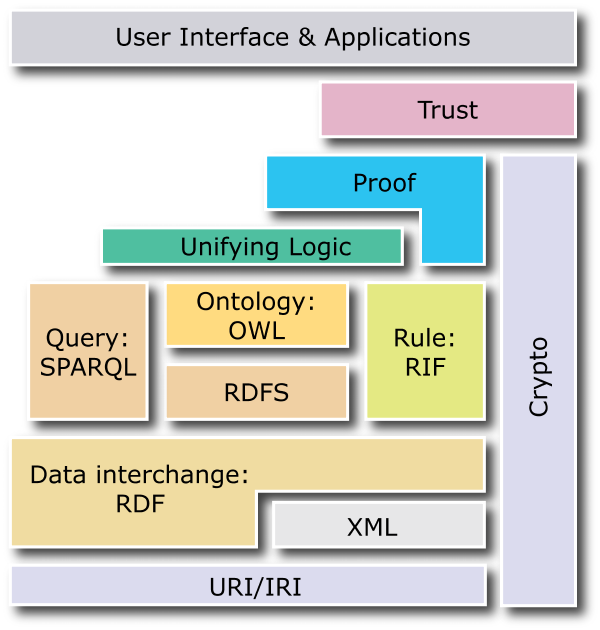
\includegraphics[width=0.7\linewidth]{chapters/background/img/layerCake.png}
\caption{The Semantic Web layer cake.}
\label{fig:swlayercake}
\end{figure}

\subsubsection{The Resource Description Framework (RDF)}

``The Resource Description Framework (RDF) is a framework for representing information in the Web.'' \cite{Klyne2004} It defines a standard model for representing and exchanging information on the Semantic Web. The RDF Specification has been a W3C Recommendation since 1999 \cite{Lassila1999}, with the latest version being a suite of six W3C Recommendations\footnote{\url{http://www.w3.org/standards/techs/rdf}}, published in 2004̇. 

\lstset{
	caption={RDF example represented in Turtle.}, 
	label=lst:rdfex,
	language=turtle
}
\setlength\parindent{0in}
\begin{minipage}[htb]{\linewidth}
\begin{lstlisting}
@prefix ex: <http://www.example.org/RDFexample#> .
@prefix rdf: <http://www.w3.org/1999/02/22-rdf-syntax-ns#> .
@prefix rdfs: <http://www.w3.org/2000/01/rdf-schema#> .
@prefix foaf: <http://xmlns.com/foaf/0.1/> .
@prefix bibo: <http://purl.org/ontology/bibo/> .
@prefix dcterms: <http://purl.org/dc/terms/> .

ex:doctorow a foaf:Person ;
   foaf:name "Cory Doctorow" ;
   foaf:firstName "Cory" ;
   foaf:surname "Doctorow" ;
   foaf:homepage <http://craphound.org> ;
   foaf:made ex:ftw .
ex:ftw a bibo:Book ;
   dcterms:title "For The Win" ;
   foaf:maker ex:doctorow ;
   bibo:issn13 "9780765322166" .
\end{lstlisting}
\end{minipage}
\setlength\parindent{0.21in}

RDF is designed to allow flexible representation of information. The underlying structure of any data represented with RDF is a graph, which is a collection of triples. Each triple represents an RDF statement, and is made up of a subject, a predicate (or property), and an object. An example is shown in Listing~\ref{lst:rdfex}. A triple can be seen as a graph made of two nodes, the subject and the object, connected through an arc, represented by the predicate. Thus, a set of triples can be represented as a graph by the corresponding set of nodes and arcs (see Figure~\ref{fig:rdfex} for an example). 
Any information about a resource can be expressed through triples, including information about a triple, through a process called reification. While a powerful feature, reification adds complexity, and is usually used sparsely. An extension to RDF allows statements to be grouped in \emph{named graphs} which helps avoid the use of reification to store meta-information about triples, like provenance for example.

\begin{figure}[th]
 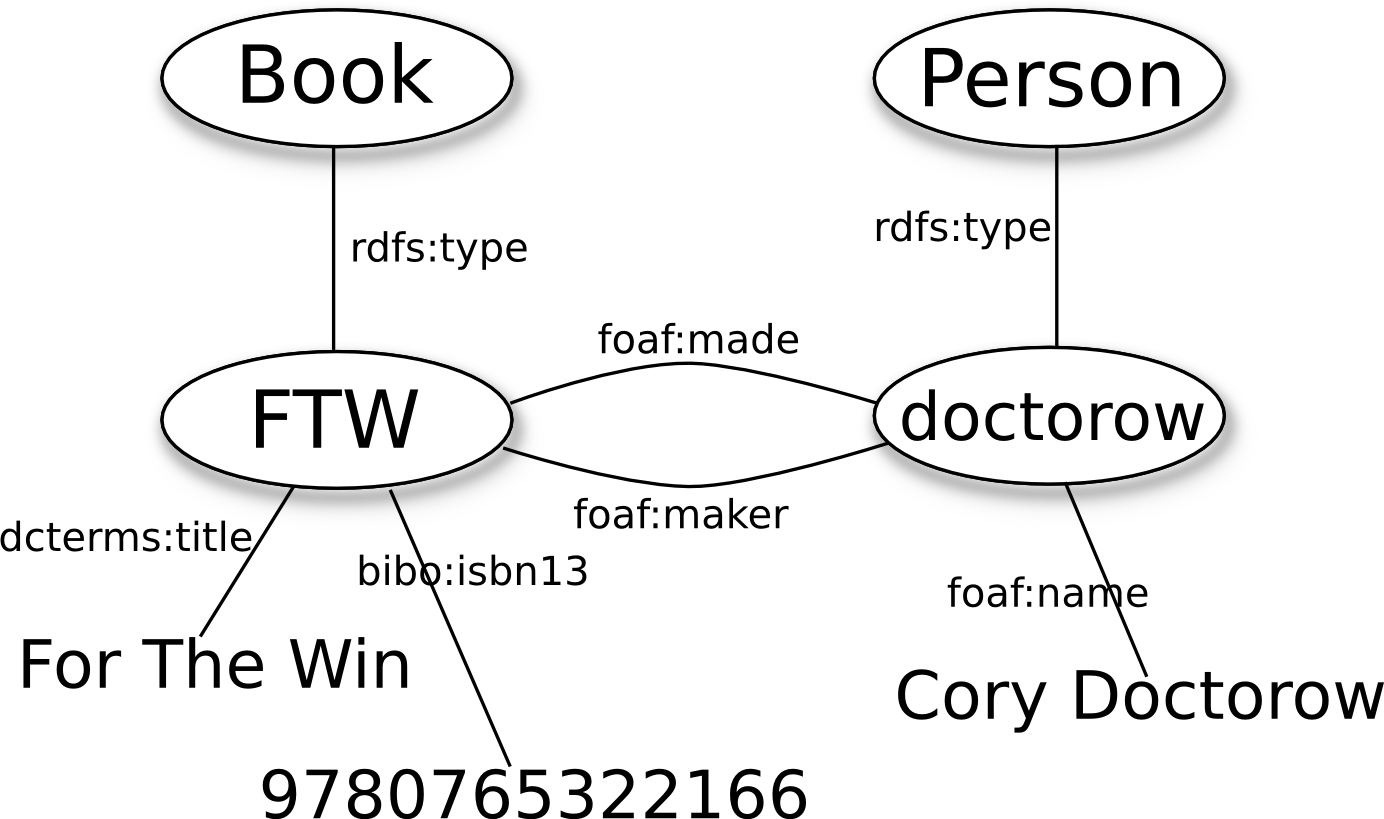
\includegraphics[width=0.8\linewidth]{chapters/background/img/rdfex}
\caption{RDF example represented as a graph.}
\label{fig:rdfex}
\end{figure} 

The RDF specification defines three types of elements: 
\begin{itemize}
 \item identified resources, which are represented by a URI. They can appear on any position in a triple.
 \item unidentified resources, called blank nodes, which cannot appear as predicates in triples. They are unnamed nodes within a graph, and using them can pose problems, thus it is discouraged \cite{Bizer2007}.
 \item literals, which can only appear as objects in a triple. Literals represent values of properties. They can be typed, using XML Schema datatypes, or can have a language tag.
\end{itemize}

RDF is a data model which can be serialised in several ways. The most popular serialisation of RDF was first RDF/XML \cite{Beckett2004}, due to the popularity and familiarity of XML. More recently however, other serialisations, more suitable for human consumption, have become preferred: N-Triples ~\cite{Grant2004}, Turtle \cite{Beckett2007}, and N3 \cite{BernersLee2006b}. RDFa \cite{Adida2008} is another syntax for RDF, which allows embedding of RDF statements in HTML pages. In the following chapters of the thesis, we will use the Turtle notation in listings.

SPARQL \cite{Prudhommeaux2008} is the recommended query language for RDF. Other query languages for RDF exist, including: 
\begin{itemize}
 \item RDF Query Language (RQL) \cite{Karvounarakis2002}, 
 \item Sesame RDF Query Language (SeRQL) \cite{Broekstra2003}, 
 \item RDF Data Query Language (RDQL) \cite{Seaborne2004}.
\end{itemize}

\subsubsection{Ontologies and Vocabularies}

RDF gives us the means to represent information in a unified way. However, this is not enough to make the information understandable to machines. Something more is needed, and that is a common, agreed-upon, and shared vocabulary to refer to things. This is represented by the ``Ontology'' layer in the SW layer cake. According to Gruber, an ontology is ``an explicit specification of'' [...] ``an abstract, simplified view of the world that we wish to represent for some purpose.'' \cite{Gruber1993}

RDF Schema (RDFS) \cite{Brickley2004} was created to support the use of RDF to define ontologies. The Web Ontology Language (OWL) is another formal language to define ontologies, which offers more expressive constructs than RDFS.

Both languages allow the definition of classes, hierarchies of classes, properties with domain and range, and hierarchies of properties. 

Ontologies can be: \emph{upper-level} (or top-level, or foundation) ontologies, defining high level, generic concepts, or \emph{domain} ontologies, which define concepts related to a specific, restricted domain.

Numerous vocabularies have emerged for the Semantic Web. Among them, a limited number have gained wide-spread adoption and recognition. The ones we use and refer to in this thesis are listed below:
\begin{itemize}
 \item Dublin Core Metadata Initiative (DCMI\footnote{\url{http://dublincore.org/}}) \cite{Nilsson2008} --- for ``core metadata for simple and generic resource descriptions'';
 \item Simple Knowledge Organization System (SKOS\footnote{\url{http://www.w3.org/2004/02/skos/}}) \cite{Miles2009} --- for sharing and linking data about ``knowledge organisation systems, such as thesauri, taxonomies, classification schemes and subject heading systems'';
 \item Friend Of A Friend (FOAF\footnote{\url{http://foaf-project.org}}) \cite{Brickley2005} --- for describing people and organisations;
 \item Semantically-Interlinked Online Communities (SIOC\footnote{\url{http://sioc-project.org}}) \cite{Breslin2005} --- for describing online communities; 
 \item Description Of A Project (DOAP\footnote{\url{https://github.com/edumbill/doap}}) --- for information about software projects;
 \item the Music Ontology (MO\footnote{\url{http://musicontology.com/}}) --- for ``describing music (i.e. artists, albums, tracks, but also performances, arrangements, etc.)'';
 \item GeoNames\footnote{\url{http://www.geonames.org/ontology/}} --- for geographic information.
\end{itemize}

\subsection{Linked Data}
\label{sec:ld}

The term Linked Data was first introduced by Berners-Lee in 2006 to define a set of best practices for publishing data on the Web \cite{BernersLee2006}. They became known as the ``Linked Data Principles'' and describe the recommended way to publish and connect data on the Web, so that ``it is machine readable, its meaning is explicitly described, it is linked to other external datasets and can in turn be linked from external datasets''.

In addition to these principles, the more recent Linking Open Data\footnote{\url{http://linkeddata.org}} project enables the creation of a huge amount of interlinked RDF data on the Web, from various open datasets, ranging from Health Care and Life Sciences (HCLS) information to the BBC programmes. 


\section{Personal Information Management}
\label{sec:pim}

Personal Information Management has been a concern and research topic from the early days of computing, and even before. Bush's Memex (see Section \ref{sub:bush}) was the first envisioned automatised PIM system. It acted as an extended personal memory, an archive of all the personal information, and a holder of explicit links between this information. The vision of the Memex was carried over through the evolution of the personal computer  (and recently many other personal devices as well). 

\subsection{Personal Information}
\label{sub:pi}

To better understand what Personal Information Management is, we first need to define \emph{personal information} in this context. There is a large body of research done in the area of PIM, and as such, there are several definitions of what personal information is, some more restrictive and some more broad. However, an important distinction to make is that personal information is not \emph{Personal Identifiable Information (PII)} which is a piece of data that uniquely identifies a person. Personal information is also not restricted to private information. It is true that some of our personal information is private, but not all of it. As \cite{Lansdale1988} described: ``personal information is information not in a sense that it is private, but that we have it for our own use. We own it and would feel deprived if it would be taken away.'' In his Ph.D. thesis, Boardman defines Personal information as ``information owned by an individual and over which this individual has a direct control'' \cite{
Boardman2004PhD}.

Jones \cite{Jones2007PIMBook,Jones2008KFTFBook} defines personal information from the point of view of its relation to a person, through six overlapping categories:
\begin{itemize}
 \item \emph{controlled by (owned by) me} --- the information the person keeps, directly or indirectly, for personal use;
 \item \emph{about me} --- the information about a person, but available to, and possibly under the control of others;
 \item \emph{directed toward me} --- email received, or advertisements seen, this information itself may not be relevant to the person, but its impact is personal;
 \item \emph{sent (posted, provided) by me} --- this information is no longer under the control of the user after it has been sent;
 \item \emph{(already) experienced by me} --- like a radio show, a book read, or a web page seen, this information may or may not be under the control of the person;
 \item \emph{relevant (useful) to me} --- this category includes information from the previous categories, but also new information, which has not been seen before, but is relevant or useful.
\end{itemize}
In this thesis, when we refer to personal information, we mean it in the broadest sense of the term, as in this definition by Jones.

\subsection{Personal Information Management}
\label{sub:pim}

The goal of PIM is to help the user find the right information at the right time for the task at hand, with as little effort as possible. The means to achieve this is to enable the user to organise the information better, and over time, organisation has transformed from the means to a goal in itself. 

As with the definition of personal information, there are several definitions for PIM. \cite{Lansdale1988} describes it as ``the methods and procedures by which we handle, categorise, and retrieve personal information on a day-to-day basis.'' \cite{Barreau1995b} defines a PIM system as ``an information system developed by or created for an individual for personal use in a work environment.'' According to \cite{Boardman2004}, PIM is ``the collection, storage, organisation and retrieval of items of digital information (e.g. email, files, appointments, reminders, contacts, bookmarks) by an individual in their personal computing environment.'' \cite{Jones2008KFTFBook} formally defines PIM as referring to ``both the practice and the study of the activities a person performs in order to acquire or create, store, organise, maintain, retrieve, use and distribute the information needed to meet life's many goals (everyday and long-term, work-related and not) and to fulfil life's many roles and responsibilities.'' 
\cite{Lansdale1988} describes PIM in relation to psychology --- showing how classification is a difficult activity due in part to ambiguous terms, and how memory affects recall.
The term ``mental model'' was coined by \cite{Craik1943} and has been used and studied \cite{Norman1983,Paivio1986,Johnson-Laird1989} since then. Research in psychology and cognitive sciences has shown how mental models are created, how they evolve and how they support learning, collaboration and information retrieval \cite{Jarvelin2003,Payne2003,Jones2011}. An overview of the field and its connection to PIM is presented in \cite{Nadeen2007}. Conceptual models have been described and used by both Bush and Engelbart as foundations for their work.

According to \cite{Barreau1995b}, PIM systems can be categorised using the following criteria, which are still valid today:
\begin{itemize}
 \item \emph{acquisition} -- how and what information enters the system; 
 \item \emph{classification and organisation} --- how the information is grouped and labelled;
 \item \emph{storage} --- how the information is stored for later retrieval; 
 \item \emph{maintenance} --- how the information is updated and migrated if needed; 
 \item \emph{retrieval} --- how the system enables retrieval of information at the appropriate time, this being one of the most important functions of PIM, the majority of the other characteristics revolving around and working towards the eventual retrieval of information; 
 \item \emph{output} --- how the system can answer queries related to the user's information and context.
\end{itemize}

Many user studies have been conducted to determine the requirements for different PIM tasks, how people tend to solve problems that occur frequently, how they generally organise their information --- be it on their physical workspaces or on their virtual ones. One of the most notable studies is that of \cite{Barreau1995a}, which ``investigated information organisation practices of users''. They categorise the information handled by the participants into three categories:  ephemeral, working, and archived --- with the very interesting observation that one of the concerns raised by the study was the large amount of ephemeral information that the users had to cope with, which accumulated and cluttered the workspace. The management of this ephemeral information is the focus of the study by \cite{Bernstein2008} on ``information scraps'', defined as ``is information items that fall outside all PIM tools designed to manage them''.

Another finding of the Barreau and Nardi study was the ``preference for location-based search for finding files'' and ``the critical reminding function of file placement''. 
\cite{Fertig1996a} argue the need for better systems for organising the information than those offered by the desktop metaphor at that time. They suggest that although people make the best of the tools they are given, that does not mean that the tools are suitable for the task, and that better alternatives should be researched. Their examples include the Lifestreams \cite{Freeman1995,Fertig1996b} system which proposes a chronological organisation of documents, and the MIT Semantic File System \cite{Gifford1991} which offers an associative organisation similar to the vision of the Memex. \cite{Civan2008} describes another user study focused on comparing location-based organisation in folders with category-based organisation with the use of tags, in the context of email management. The study by \cite{BlancBrude2007} determines which attributes enable the best re-finding of information in a PIM system, and how tools for information retrieval could be improved by supporting the combination of attributes most 
likely to lead the user to the desired result.

Many applications have been created for each of the supporting activities of PIM: document management, contact management, email, calendaring, task management. These applications serve their chosen domain well, offering rich sets of features and capabilities. However, the information that each of them handles is rarely used on its own, or separate from the rest, thus integrated information is a requirement of PIM. Additionally, a prevalent problem is the locking of information in application specific repositories, and in application specific formats, making integration difficult. Another problem is information fragmentation in multiple places and applications. \cite{Boardman2004} describes a cross-tool study to determine how users manage their personal information within applications and across PIM tools. The findings show that most of the time the information is classified in similar hierarchies, and as a result there is duplication of the work required to organise information in each tool. From another 
longitudinal study Boardman classifies users into categories, depending on their behaviours, and presents insight into how these behaviours evolve over time. \cite{Kaptelinin2007} describe two different approaches to information integration: through a single ``mega-application'' which supports multiple PIM activities, or through the coordination of several applications in a unified workspace. The problem of information fragmentation and solutions for unification or integration are also found in \cite{Karger2006,Karger2007}.

Another challenge relevant to building and improving PIM tools is how to evaluate them. The problem has been discussed by \cite{Whittaker2000} and also by \cite{Kelly2006,Elsweiler2007,Bernstein2007}. The main difficulty o\-riginates from the personal nature of the information handled by the systems, and the familiarity of the users with this information, familiarity which cannot be replicated in artificial conditions. It extends to the fact that the tasks that users work towards solving with the PIM systems are also highly personal, thus artificial tasks for the purpose of evaluation would not yield clear results. 


\section{Conclusion}

In this chapter we presented the terminology that is used in the thesis, both from the area of the Semantic Web and that of Personal Information Management. We gave an overview of the Semantic Web, its evolution from the document Web, and its core technologies. 
We have also described what ``personal information'' refers to in the context of Personal Information Management, and what are the research areas, and challenges of the domain. 

We continue to show in the next chapter how the semantic technologies have been applied on the desktop and to PIM, to create Semantic Desktop systems. These systems are apply the most basic elements of semantic technologies, the categorisation of entities into classes and the explicit specification of links, to representing the mental models with the help of computers. 

\chapter{The Semantic Desktop}
\label{ch:sd}

\begin{flushright}
 \textit{Based on ``Knowledge Management on the Desktop'' \cite{Dragan2012}\\published at the 18th International Conference on Knowledge Engineering and Knowledge Management (EKAW2012)}
\end{flushright}

Having defined the semantic technologies used on the Web, we continue in this chapter to show how they have been applied on the desktop and to Personal Information Management, to create the Semantic Desktop. We provide an in-depth overview of existing Semantic Desktop features and architectures, since our work is grounded in the framework given by the Semantic Desktop, enhancing and complementing its features. 

\section{Visionaries}
\label{sec:visionaries}

The ideas behind the Semantic Desktop have been around for much longer than the actual devices (personal computers, netbooks, tablets or even smartphones) on which they run. The common problem the Semantic Desktops are trying to solve is finding better ways for knowledge workers to manage the ever-growing amount of information they need to work with and process. 
The most relevant historical precursors of the Semantic Desktop are, in chronological order:

Paul Otlet's Universal Bibliographic Repertory is a Belgian enterprise from the end of the 19th and the beginning of the 20th century, trying to set up a comprehensive system of all the bibliographic knowledge available, and keep it up to date as new knowledge appeared. It used a system of interlinked index cards, with reference codes pointing to relevant information, thus creating the first network of knowledge, although not an machine readable one. Despite not being widely recognised as such, it does represent the beginning of standardised knowledge and information management.

Vannevar Bush's Memex --- cited by most ``modern'' Semantic Desktops as inspiration, describes a first vision for a truly personal system for interlinking information. Although Bush's seminal paper ``As We May Think'' was published in 1945, his work on the Memex started well before that.

Douglas Engelbart's Augment --- built on the vision of Memex, the Augment was the first ``real'' functional system. As of 2012, it is still being used by its creator, despite being created in the early 1960s. Engelbart's ideas on bootstrapping are also relevant in the evolution of Semantic Desktops. 

Theodor Nelson's Xanadu --- imagined at roughly the same time as Augment, the Xanadu system was never completed. However, the ideas behind it inspired many of the future developments that shaped the Web and many technologies that exist today.

\subsection{Paul Otlet (1868 - 1944)}
\label{sec:otlet}

Although Bush, Engelbart and Nelson's works are usually cited as inspiration and background in most works about the Semantic Desktop, Paul Otlet's work is relevant through its influence on them. His work anticipated many of the features of the other historical systems described here.
Otlet, a Belgian lawyer turned bibliographer, was one of the (grand-)fathers of information science. He wrote numerous essays on the need for an international system for handling, indexing, linking, and accessing information, as a way of containing and managing the vast knowledge produced by man. Otlet created the Universal Decimal Classification (UDC) as the solution to the problems he described in his essays. The UDC pioneered the use of standardised index cards which allowed for continuous interlinking and referencing of entries, and represents one of the first faceted classification systems. The UDC was used to create a huge database called the Universal Bibliographical Repertory, which had 15 million entries by the late 1930's. The UDC is still in use throughout the world, although in revised and updated forms. It can be seen as precursor to high level taxonomies of concepts for classification, with notions of ``narrower" and ``broader" subject terms. 
Otlet's activity and vision are reflected in his chef d'oeuvre ``Trait\'{e} de documentation'' \cite{Otlet1934}. It is seen as precursor and motivator to the hypertext, mark-up languages and even the Semantic Web.

\subsection{Vannevar Bush (1890 - 1974) and the Memex}
\label{sub:bush}

Bush was an American scientist and public figure. During the World Wars he coordinated researchers from many domains, towards applying scientific advances to warfare and defence. He was an unofficial scientific advisor to two US presidents\footnote{Franklin D. Roosevelt and Harry S. Truman}, and led several institutions and committees, along with initiating and supporting the creation of the National Science Foundation in the United States. Throughout his career Bush passionately supported collaboration between researchers, which he saw as the fastest path to the progress of humanity. He went as far as to propose an exchange of scientific results between the United States and Russia during the Cold War, to promote collaboration and prevent the atomic bomb race.

\subsubsection{``As we may think'' (1945)}

Bush was deeply concerned with the continuation of the collaboration between scientists after the Second World War was over. Himself a scientist, Bush was also painfully aware of how the progress in science meant that more research results are published than can be followed, and that because of old and inadequate publishing systems, as well as the sheer amount of information, much of the new research is unreachable, lost or overlooked. 

In a lengthy essay titled ``As We May Think'' \cite{Bush1945}, published in The Atlantic Monthly and later in Life, Bush describes several devices, possible inventions of the future, as solutions to the problems of research publishing and as teasers of tantalising scientific advances. Some of the devices may seem amusing in the context of current developments, but looking back, they are remarkable through their accuracy and foresight. 
The most famous of the devices described by the article is the Memex --- ``... a future device for individual use, which is a sort of private file and library'', ``... a device in which an individual stores all his books, records and communications, and which is mechanized so that it may be consulted with exceeding speed and flexibility''. Leaving aside the physical description of the device, which was envisioned in the form of a desk with screens, drawers for storage, a keyboard, buttons, and levers, Bush has more or less described the functions of a present day personal computer --- a device where we store and consult personal documents and communications. Furthermore, the Memex, attempts to mimic the way associations in the brain works, by using ``associative trails'' of connected things. The trails can be created, modified, browsed, shared and collaborated on. ``Associative indexing'' was ``the essential feature of the Memex.'' 
Bush presents a greater purpose for his Memex --- creating new forms of linked (associative) encyclopaedias. They would serve as a record of the human knowledge accumulated over time and would ``accelerate technical progress''. 

Although the article was published in 1945, Bush had been working on the idea of the Memex for many years before, and although there are no clear indications of any influences from Otlet's work, their higher end goals are similar. 
Some claim that Otlet's work was indeed known to Bush, indirectly through Watson Davis' visit in 1932 and there is some overlap between the works of the two to support it\footnote{\url{edwardvanhoutte.blogspot.com/2009/03/paul-otlet-1868-1944-and-vannevar-bush.html}} \cite{Veith2006}.
However, Bush writes against indexing systems, that he sees as artificial and cumbersome, and one of the reasons why information is hard to find. But the Memex could benefit from something like Otlet's UDC, a common system for classification of the trails. The trail names used in the Memex are instead highly personal and cryptic, which can become a problem when it comes to sharing the knowledge \cite{Buckland1992}.

The elegant ideas behind the Memex influenced the fields of information science and information management, and the development of personal computing, hypertext and semantic technology. The Memex is the first Semantic Desktop described in the literature, and although it was never realised, it has influenced the works of both other two visionaries included in this section, Douglas Engelbart and Ted Nelson.

Bush continued to work on the project, and wrote further articles on the Memex, like ``Memex II'' from 1959, and ``Memex Revisited'' from 1967, which are included in the book \cite{Nyce1991}.

\subsection{Douglas Engelbart and Augment}
\label{sub:engelbart}

From a desire to ``improve the lot of the human race'' \cite{Goldberg1988}, Douglas Engelbart has devoted his career to ``augmenting the human intellect''. In pursuit of this goal, he invented many devices that greatly influenced the way we work with computers today: the mouse, the window, the word processor, video conferencing, remote procedure calls, hypertext, and more. However, all these notable advances were just first steps towards his greater purpose, that of achieving an augmented human intellect.

\subsubsection{``Augmenting the Human Intellect'' (1962)}

The 1962 report ``Augmenting the Human Intellect'' \cite{Engelbart1962} describes a conceptual framework for his research, presenting the details of the H-LAM/T system (Human using Language, Artefacts, Methodology, in which he is Trained). It defines four classes of possible augmentation means, through intertwining artefacts, language, methodology and training. It also discusses thought process and repertoire hierarchies, and how they influence problem-solving capabilities. Furthermore, Engelbart defines mental structures, concept structures and symbol structures, and their relationship to each other. He introduces the hypothesis that ``better concept structures ca be developed -- structures that when mapped into a human's mental structure will significantly improve his capability to comprehend and to find solutions within his complex problem situations.''

The report thoroughly quotes and discusses Bush's ``As We May Think'', which Engelbart believes ``to make a very convincing case for the augmentation of the individual intellectual worker.'' He focuses on Bush's description of the Memex, and highlights how the device fits within the conceptual framework of augmentation. He also shows how the associative trails pioneered by Bush map to the concept and symbol structures from H-LAM/T, and how they can be evolved further, in the context of a note-card system.
Apart from the high-level ideas that precede and build up to the ideas of the Semantic Desktop, the Augment report also describes and motivates the need for a well designed semantic model for such a system. In an exercise of forethought, Engelbart says that classification ``might be the most significant part of the work.'' He envisions that the extra effort required ``to form tags and links [...] consciously specifying and indicating categories'' would be rewarded by the capacity gained by the computer to understand and perform more sophisticated tasks. He describes the ontology creation model - establishing the categories and relations between them, dealing with and removing semantic ambiguity.

\subsubsection{``A Research Center for Augmenting Human Intellect'' (1968)}

The \cite{Engelbart1968} report describes the system that was shown at the 1968 Fall Joint Computer Conference in what has become known as ``the mother of all demos'' because of the size, novelty and sheer number of innovations shown together at one time. The demo, and report, are outstanding for many reasons --- the infrastructure required to run it, the number of people involved, the introduction of the mouse, the collaborative work environment, the first word processing software, and many more. However, from the Semantic Desktop point of view, the spectacular part comes from its realisation of the conceptual framework detailed in the 1962 report \cite{Engelbart1962} --- the introduction of explicit hierarchical structuring of information --- ``we adopted some years ago the convention of organising all information into explicit hierarchical structures, with provisions for arbitrary cross-referencing among the elements of a hierarchy''; ``the symbols one works with are supposed to represent a mapping of one'
s associated concepts, and further that one's concepts exist in a network of relationships.''
Allowing the creation of arbitrary links between elements of the hierarchy, and providing unique names for entities for better and faster access, represents the realisation of Bush's associative trails and makes Engelbart's On-Line System (NLS) the first functional predecessor of a Semantic Desktop. The semantics are limited to the network of statements in files, but this is an important first step towards deeper interlinking.

\subsection{Theodor Nelson and Xanadu}
\label{sub:nelson}

By his own account, Nelson was not an engineer but a philosopher and cinematographer, and ``a computer fan, computer fanatic if you will'' \cite{Nelson1974}. However, he saw the potential that computers had beyond data processing and computation. He envisioned a way of using the computer as ``an adjunct to creativity'' for writing and personal information management, in the style of Bush's Memex for personal use. 

Nelson foresaw the information overload crisis we are facing, and many of the developments that created it: the personal computer, enhanced communications, digital publishing, virtually infinite storage. He has imagined a solution to the problem ---  a ``psychic architecture'' of a system \cite{Nelson1973}, where psychic refers to ``the mental conceptions and space structures among which the user moves''. 
The idea was embodied in a system called Xanadu, the specification and requirements of which are detailed as early as 1965 in \cite{Nelson1965}. Xanadu transformed over time, from an ``effort not to forget'' and to organise personal information better, into a vision of unrestricted linking of passages of text.

Nelson proposes for Xanadu a new file structure called ELF (evolutionary file structure) made up of entries, lists and links, as a way or realising the associative trails of the Memex. The zippered list structure described by him allows ``any two entries to be connected'', by ``link-modes having different meanings to the user'' --- similar to how we use RDF in current semantic systems. 
Nelson shares with Engelbart the credit for the invention of hypertext (hypermedia and hyperfilm), where ``hyper'' has roughly the mathematical sense of ``extended, generalised, and multidimensional''. Hypertext's purpose was to reflect ``the real structure of the thoughts expressed'' by users.
The freedom to link anything with his version of hypertext was supporting what Nelson called transclusion, the process of including something by reference rather than by copying --- ``quoting without copying''. Already in his 1973 article \cite{Nelson1973} he mentions concerns for the security  of hyperlinked data, and based on transclusion, Nelson invented a new type of copyright management called transcopyright.
Zippered lists also have evolved into zzstructures, which are at the basis of ZigZag hyperstructure toolkit and the ZigZag personal environment \cite{Nelson2004}.

The Xanadu system was in development for many years, but it has never become fully functional. Despite it not being a success, the vision behind it has inspired many dedicated followers and influenced today's world of personal computing. 

\subsection{Influences and Influencers}

There is a distinguishable network of influence in the domain of networks of knowledge.

It is uncertain if Otlet's work has in any way influenced the inception of the Memex across the Atlantic at the same time, but the idea is supported by the fact that he ``reported enthusiastically on experiments with other bibliographical applications of technology, especially microfilm'' \cite{Goldschmidt1982,Rayward1990}. Furthermore, ``in the early 1930's Otlet began to speculate about how a wide range of then experimental technology --- radio, cinema, microfilm, and television --- could be combined to achieve a new complexity and variety of functionality in information searching, analysis, re-structuring and use'' \cite{Rayward1991}.

The influence of Bush's Memex on the works of Engelbart and Nelson is, however, undisputed, and stated by both in their writings. The directions were different though:  Engelbart NLS was designed by engineers, focused on their needs, and encouraging collaboration. Xanadu on the other hand was intended for personal use, for capturing the train of thought of one user and to serve as an extended memory. Some of the features envisioned by Nelson for Xanadu were incorporated in Engelbart's NLS --- the ability to link paragraphs of text, revise documents in real-time by moving pieces of text on the screen, preserve and track changes.


\section{A Survey of Semantic Desktops}
\label{sec:sd}

We have covered so far the futuristic systems of the past and the visionaries who imagined them, like the Memex, which since 1945 have been an inspiration for most of the work in personal computing and personal information management. We have also briefly described the Semantic Web and its technologies. We will now show through a list of “modern” Semantic Desktops how semantic technologies are put to use in those systems to realise the vision of the Memex, and more.

\subsection{Common Challenges}
\label{sec:sdgoals}

The term \emph{Semantic Desktop} was coined in 2003 by Decker and Frank and was taken up first by Sauermann in Gnowsis \cite{Sauermann2003}. 

The [Social] Semantic Desktop saw the fastest rise and uptake during the 2004 -- 2009 period, when most research work was put into the development of systems and applications, new and improved algorithms to support knowledge work. 
These systems and tools were aiming to solve similar problems as was the Memex before them: supporting and improving knowledge work by mimicking the way the brain works --- using Bush's associative trails reworked with the help of the semantic technologies. 
The fast growth of the digital world, while providing easier access to information and communication, has created new problems, foreseen by Nelson in the 70s: there is so much information available that it becomes unmanageable. 

Thus, the challenges that the Semantic Desktops aim to solve can be described as follows:
\begin{description}
 \item[Information overload] caused by the ease with which information can now be generated, shared, stored and accumulated. The amount of information that we see, receive, create every day is enormous. While the storage and processing capacity of hardware has increased many-fold, re-finding stored information has become a more complex task. The challenge is to enable users to manage this large amount of information better, while not spending more time and effort organising it. 
 \item[Data silos] are created by desktop applications which store their data in proprietary  formats, in storage inaccessible to other applications which could possibly reuse that information, thus each mus recreate it in their own formats and store it in their own walled repositories. 
 The negative effects of this vicious circle are \emph{data duplication}, and \emph{disconnected information}. Having the same data in multiple applications leads to difficulties in keeping it up to date and synchronised. Additionally, having pieces of information relating to the same object or entity spread over several locations and tools makes working with that information more difficult, as it requires opening and browsing through several folder hierarchies and application structures, as well as piecing together the information every time it is needed. The challenge presented by data silos is to give users a unified and consistent view over their data, regardless of its source and location. 
 \item[Dynamic data] means that information changes over time, and thus it can become deprecated. Using deprecated information can have undesired effects, like sending emails to an old email address of a contact. The data silos problem above adds complexity to this --- \emph{duplication of data} in various applications makes it more difficult to decide which version is correct; \emph{disconnected information} means that when a piece of information changes, care must be taken so that the changes are made in every place where the information is kept, increasing the effort required.
 \item[Associative trails] as those described by Bush, follow the way we think about things, by connections and associations, unconstrained by the way the information is stored or presented in various applications. This point is also related to the data silos issue. As we discussed above, studies showed that the way we form mental models and work with information is task and data centric. As long as data is disconnected and locked away in application repositories, explicit associative trails can only be fragmented, short and thus hurting productivity. 
\end{description}

The 2004 white paper by \cite{Decker2004} ambitiously describes a solution, the Social Semantic Desktop as ``a novel collaboration environment, enabling the creation, sharing and deployment of data and metadata'' and names the sources that would contribute to the development of such a system: ``Semantic Web, Peer-to-Peer Networks, and Online Social Networking.'' From the point of view of the future Social Semantic Desktop, the Semantic Desktop was just one piece of the puzzle, its function being that of a smart personal information management tool, that provides a common vocabulary, creates and maintains a network of interconnected personal information, stores it and gives users access to it through search and browsing.

The 2005--2006 workshop series on the Semantic Desktop, and the 2005--2008 series of hands-on workshops\footnote{\url{http://semanticweb.org/wiki/Semantic\_Desktop\#Dissemination\_activities}} served as a catalyst for early ideas and brought together researchers interested in the topic, who were already working on relevant projects. Some of the systems that are described below were introduced at these workshops: \emph{IRIS}, \emph{DeepaMehta}, \emph{HyperSD}, \emph{WonderDesk}. The workshops saw also the presentation of stand-alone semantic applications like the Semantic Clipboard \cite{Reif2006}, Beagle++ \cite{Brunkhorst2006}, Semantic Wikis \cite{Oren2005,Aumueller2005}, Semantic Instant Messaging (SAM \cite{Franz2005}, Nabu \cite{Osterfeld2005}), semantic federation \cite{Park2006}, semantic search and ranking \cite{Chirita2005}, and trust \cite{Noh2006}.

\subsection{Semantic Desktop Systems}
\label{sec:sdsystems}

In this section we present a review of existing Semantic Desktops. The NEPOMUK project is described separately in Section \ref{sub:nepomuk}. 

The Semantic Desktops presented here have the same common goals, and tackle by some extent the same challenges we described in Section \ref{sec:sdgoals}. Some of the systems cover a broad spectrum of activities, aiming for a general solution, while others are focused on precise PIM tasks like email or task management. 

We begin by describing the systems, along with their characteristics and features, and then continue by delving into the details of the architecture, services and ontologies for a subset of them. We start with the more relevant ones, which we describe in more detail. We then continue with other systems providing similar functionality. The list is ended by very specialised systems or applications, with semantic features.

\subsubsection{Haystack}

The Haystack system came out of MIT's Computer Science \& Artificial Intelligence Laboratory (CSAIL) as early as 1997. It started as a personal system for Information Retrieval, where users manage their own private information \cite{Adar1999}, and the system adapts to the users' behaviour. Although not explicitly stated, from the beginning Haystack has been a semantic system, as it created and saved metadata links, or associations between things in the user's corpus, and allowed these links to be followed from one document to another. The connections are made either by inspecting the content of the documents, or by tracking the user's activity and inferring the connections. The user can also annotate content with metadata. 

The architecture of the system evolved over time, but the overall structure remained the same \cite{Huynh2002,Quan2003b} --- a three-tiered design. At the bottom there is a storage layer for the user's content --- initially a database, later, an RDF store. On top of the storage, Haystack provided a basic data model for the objects, metadata and links; later it moved to RDF for describing the data. The RDF model is general, but it allows customisation by users \cite{Karger2006}. The top level is made of client applications which can have one of several roles: \begin{inparaenum}[(i)] \item proxies for extracting information from existing unstructured sources like user applications or the Web; \item connectors for linking already extracted information; \item observers of user actions \end{inparaenum}. There are also client services through which the user can interact directly with the data --- modify it, search it or visualise it. 

\subsubsection{Stuff I've Seen (SIS)}

The Stuff I've Seen (SIS) system is presented by \cite{Dumais2003} as a solution to re-finding previously seen information, be it in an email, on a web page or in a document. The authors recognise the problem of data loss due to ``the multiplicity of independent applications used to manage information each with its own organisational hierarchy'' and ``the limited search capabilities'' they offer. SIS was not meant to be a new PIM application, but a unified point of access to existing content from other applications. It uses a central index and provides a common search interface over existing information sources. It aids re-finding of information by employing contextual cues in the search interface. 

Developed at Microsoft, the system is based on the Microsoft Search indexing infrastructure, thus having access to functions of the operating system inaccessible to third-party applications. The architecture is modular. Five main components are chained to feed data extracted from various sources into the index. There is no mention of any semantic technologies being used, although some structured information is extracted: type of the resource, relations to other resources, like sender of an email and author of a document. The structures are then used to provide faceted query refinement. Some extraction of information from the content of the files is done with natural language processing. SIS also allows users to create metadata annotations on their content, which is an important first step towards creating semantic relations.

An extensive user evaluation of the system explored the best ways of presenting the search results, and determined which are the most common ways of searching for information. 
It found that time and people are important cues in re-finding, and thus should be included as part of the saved context. 
The importance of the time dimension is further studied in \cite{Ringel2003}, also based on the SIS system. 
Lifestreams \cite{Freeman1995,Fertig1996,Freeman2007} proposed a chronological ordering of information and a totally reworked metaphor for the desktop, based on time as a storage model. 

\subsubsection{MyLifeBits}

MyLifeBits \cite{Gemmell2002,Gemmell2003a,Bell2007} is another project by Microsoft Research, which uses the Memex as a blueprint for a digital personal store \cite{Gemmell2006}. The team behind the CyberAll project \cite{Bell2001}, which then was continued by MyLifeBits, started an ambitious task: ``to digitally store everything from one’s life, including books, articles, personal financial records, memorabilia, email, written correspondence, photos (time, location taken), telephone calls, video, television programs, and web pages visited.'' \cite{Bell2004}. The initial focus was on improving the methods for capture and storage, populating a personal ontology with digitised information from many sources. The following step was devising methods for using the information gathered --- ``tools [\dots] for annotation, collections, cluster analysis, facets for characterising the content, creation of timelines and stories'' \cite{Bell2004}.

MyLifeBits does not impose a strict single hierarchy over the user's data, but uses links and annotations to organise the objects, and collections to group them. The annotations and links play an important role in the system. In the style of Nelson's transclusion, the links are bidirectional, and serve as well to establish ownership of connected pieces of data. Annotations play several roles in the system, and are considered important especially for non-textual resources like audio, video and images, as they enable functionalities on these resources, like text search, and story-telling, which otherwise are not possible. The system includes features aiming to make annotation as easy as possible --- bulk annotation, predefined annotations, audio annotation. Collections are a special type of annotation. They are a way of supporting a loose hierarchy, without enforcing it. Overlapping collections are allowed, as well as resources which do not belong to any collection. ``Fluid'', or virtual collections are 
also supported, by saving and reusing a query.

Another important aspect of the system is the flexible visualisation it provides. A resource or a collection of resources can be presented in several ways, as different views can give different insights into the data. ``Furthermore, the visualisation must become a UI --- the user will want to click on a row of a table or a peak in a graph and see the data behind it.'' \cite{Gemmell2003a}

MyLifeBits uses a predefined schema \cite{Gemmell2006} to describe the data collected. The schema is flexible and customisable, although the authors do not anticipate that users will make many changes to it \cite{Gemmell2003a}, as this would lead to complications in using the system. There are a set of predefined types, based on common resources available on a user's desktop. Instances of these types have unique identifiers which are used to establish the relationships. Relationship between two entities are bi-directional, and the two inverse links involved must have distinct names, e.g. ``is organiser'' and ``is organised by''.

The architecture of the system is modular, with the MyLifeBits store at the centre. The store \cite{Gemmell2003a} uses a Microsoft SQL Server database to provide the schema and store the data. 

\subsubsection{Gnowsis}

Gnowsis \cite{Sauermann2003} is one of the first implementations of a Semantic Desktop which advocated the use of Semantic Web technologies on the desktop, and the creation of a ``personal Semantic Web for PIM'' \cite{Sauermann2009}. It proposes an architecture based on a local Web server as a desktop service, while integrated desktop applications communicate with it via Semantic Web protocols. In Gnowsis we encounter for the first time the notion of \emph{desktop services} in relation to the Semantic Desktop. 

Unlike Haystack, Gnowsis proposed that existing applications be modified to work with the semantic infrastructure, rather than being replaced completely. The Semantic Desktop would play the role of integration middleware by lifting semantic data from desktop formats and storing it in a central repository accessible to the applications. The extraction of data is done by adaptors, and the resulting network of semantic information can be accessed through a Web browser type of interface, which also provides access to the underlying model. 

The semantic data is described with ontologies, and the system provides a generic personal information model (PIMO) \cite{Sauermann2006}, which is rich enough to cover most use cases, but also flexible and customisable by the users. PIMO was created with the user in mind, and to support personal mental models. 

The Gnowsis Semantic Desktop largely influenced the architecture and basic design of NEPOMUK \cite{Bernardi2008}. Its main role was that of an integration system \cite{Sauermann2005a,Sauermann2005b} for knowledge management. 

\subsubsection{Integrate, Relate, Infer, Search (IRIS)}

Another Semantic Desktop system which is all about integration is IRIS (which stands for ``Integrate, Relate, Infer, Search'') \cite{Cheyer2005}. IRIS was part of  SRI's \footnote{\url{http://www.sri.com}} Cognitive Assistant that Learns and Organizes (CALO), as a personal information knowledge source \cite{Ambite2006}. It also played the role of semantic user interface, through its embedded suite of applications. 

CALO is an intelligent agent system which consists of several connected agents \cite{Ambite2005} specialised on different areas of knowledge work --- time management (PCalM \cite{Berry2004}, PTIME \cite{Berry2005a,Berry2011}, PExA \cite{Myers2007}), task management (Towel \cite{Conley2007}, PExA), contact management, and more. The AI agents are not necessarily semantic, although they do communicate with IRIS and use the semantic information it provides in their actions. CALO not only uses the knowledge, but also creates knowledge back into IRIS.

IRIS uses ontologies to describe data --- initially a comprehensive ontology was defined, but it was replaced in favour of the Component Library Specification (CLib), the ontology used in CALO. The CLib ontology is modular just like the architecture of the system --- different agents require different ontologies: there is an Office Ontology, a Meeting Ontology, a Documentation Ontology \cite{Ambite2005}.

CALO integrated parts of Personal Radar\footnote{\url{http://www.radarnetworks.com/}} into IRIS --- the triple-store implementation (Semantic Object framework), and user interface elements. One of the key features of IRIS and CALO as a whole, is the focus on machine learning. 

\subsubsection{Semantic Explorer (SEMEX)}

The Semantic Explorer (SEMEX) is another platform for semantic PIM. The system provides on-the-fly integration of personal and public data \cite{Dong2004}, by extending a user's personal information space and providing a logical view over it. SEMEX aligns the information integration task with the user's environment, making it happen as a side effect of the normal daily tasks.

The system comes with a basic domain ontology, which can be personalised by the users either by importing new models, or by manually changing it. The authors introduce the concept of malleable schemas \cite{Dong2005c}, which can be extracted from browsing patters, or even suggested by the system based on clustering of resources. Using the ontology, SEMEX extracts semantic objects from desktop sources and stores them in a central repository \cite{Dong2005a}. 
Reference reconciliation \cite{Dong2004,Dong2005b} plays an important role in the system, particularly for the on-the-fly integration. It uses background knowledge and previous mappings for integrating external sources whose schemas might not match. 

SEMEX offers an interface, similar to that of Haystack and Gnowsis, for querying and browsing by association the underlying database.

\subsubsection{Cross-COntext Semantic Information Management (X-COSIM)}

The Cross-COntext Semantic Information Management (X-COSIM) \cite{Franz2007a} is a framework which supports seamless PIM and information linkage across different contexts that users might find themselves in. 

The system provides a reference ontology called X-COSIMO. Additional to defining concepts and relations, the ontology also describes the various possible contexts and relations between the concepts and contexts. The ontology is comprehensive, therefore to simplify its use, the system offers an application development interface called X-COSIMA, aimed at developers.

The semantic functionalities are integrated into existing applications through plugins. \cite{Franz2007,Franz2009} describes and compares COSIMail and COSIFile with their non-semantically enhanced counterparts. Like other systems above, X-COSIM provides a browser for the semantic data it handles. 

\subsubsection{Multiple Ontology based Semantic DEsktop (MOSE)}

The Multiple Ontology based Semantic DEsktop (MOSE) \cite{Xiao2005} is a multi-layered ontology framework for personal information management. The user manages the data through many \emph{Personal Information Applications} (PIA) which are specialised on certain tasks, like trip planning or bibliography management. The PIAs are the main feature of MOSE \cite{Xiao2006}. They each have their own ontology to describe the domain knowledge, a user interface and a specific workflow. The PIAs can communicate and share data through mappings of their ontologies. 

MOSE stores its data in several repositories, one for the file descriptors, one for the resources and one for tracking provenance of resources to the files they were extracted from. These repositories are populated by several services of the framework, and by the PIAs. The data can be browsed by association, modified and queried through the resource explorer, a browser-like interface. Other user interfaces to the data are provided by the PIAs, which themselves can be customised or created from scratch by the users.

\subsubsection{PlacelessDocuments} 

Placeless Documents \cite{Dourish2000} offers an alternative document management architecture, based on the flexible structure created using tags, or \emph{document properties}, not the rigid hierarchy of folders. The system, created at Xerox PARC, is based on an earlier prototype called Presto \cite{Dourish1999}. It is not explicitly a ``semantic'' framework, but it has many of the features we find in the more recent Semantic Desktops: information management based on metadata, and interconnected resources. Besides using properties to organise information from documents and emails, the Placeless system is distinctive through the use of \emph{active properties}, which store executable code, and which provide services on the documents they are attached to. These ``property-based document services are centred on the document and document activity, rather than on a separate application'' thus solving the issue of application silos and allowing the user to focus on the task. Examples of such services include 
translation, summarisation, and format conversion.

The system supports generic system properties, as well as user-generated properties which enable a personalised view of the information space of the user. The properties are stored independently from the documents they describe, in a database. 

Documents can be aggregated in collections based on their properties, they can be shared and collaborated on. The framework integrates the existing storage infrastructure available, through content providers connecting to the local file system, the web, or any network-accessible repository. Placeless Documents also integrates with existing applications which can only work with classic file systems, through the NFS protocol.

\subsubsection{WonderDesk}

WonderDesk \cite{Zhang2005} is a distributed Semantic Desktop for resource management and sharing, part of WonderSpace eScience suite. It works with scientific objects, like papers, presentations, and other research artefacts. The system provides a basic vocabulary for metadata about the eScience resources and allows different domain specific vocabularies to be loaded for each scientific discipline. A separate component of WonderSpace, a P2P super-node named WonderServer, acts as an information integrator and indexer for a network of WonderDesk peers. The hybrid P2P architecture allows sharing of information between the nodes in a network, while still functioning standalone as a Semantic Desktop. It provides annotation functionalities, as well as sharing of annotations and resources within the group, and distributed querying. 

\subsubsection{HyperSD}

HyperSD \cite{Schwabe2005} is a Semantic Desktop browser which allows navigation and access to desktop resources based on metadata about them, in the style of Haystack. The application was developed with HyperDE \cite{Nunes2005,Nunes2006}, a Semantic Web application development environment. It provides wrappers for standard desktop resources like files, contacts, events, which extract the metadata and store it alongside the schema in an RDF store. The schema is simple, reusing some properties and relations from existing Web vocabularies like FOAF. 
The interface allows faceted browsing and contextual navigation, as well as creation and editing of new items or new associations. 

\subsubsection{OntoPIM} 

OntoPIM \cite{Katifori2005} is a framework for Personal Information Management that relies on the use of a Personal Ontology. It is part of a bigger project for Task-centred Information Management (TIM), and is motivated by the same challenges as described above.
OntoPIM supports storing any object of interest from the desktop, and relating it to any concept from the ontology. The Personal Ontology is just one part of the data layer of the system. There are two other ontologies, one for domain independent objects, like documents and emails; which is mapped to another one for domain specific objects; which in turn is mapped to the Personal Ontology. The users can build and modify their model through the Personal Ontology Builder and Personalisation Tool. The system provides other services on top of the semantic data --- instance matching, semantic save, querying, mapping.

\subsubsection{The Autonomic Semantic Desktop}

The Autonomic Semantic Desktop \cite{Breitman2006} introduces a semantic layer to a self-managing (or autonomic) application architecture. The result is an integrated desktop environment capable of self-managing behaviour, which uses semantics to achieve its goal of simplifying Personal Information Management, by supporting the user in maintaining their personal information in an automatic (or semi-automatic) way. The user data is extracted from two domains, the desktop and the Web \cite{Breitman2005}, and is described by a shared ontology. The data layer is used as communication interface between a set of independent pluggable services.

\subsubsection{Chandler}

Chandler \cite{ChandlerProject} is a project that defines itself as a ``Note-to-Self Organizer'', integrating personal information from multiple applications, and supporting task management and collaboration. It does not use typical Semantic Web technologies, instead it defines its own lightweight flexible vocabulary for describing the types of data, called \emph{kinds}, as well as implementing its own data storage system. However, the ideas are consistent with those of the Semantic Desktop, integrating personal information from different sources and interconnecting it for associative browsing. The system provides a single modular user interface for the data, with different views for specific data types. Collaboration and data sharing in Chandler is realised with a client-server architecture, where the server is called a \emph{hub}.

\subsubsection{SeMoDesk}

The SeMoDesk \cite{Woerndl2008} project aims to bring the Semantic Desktop to the mobile environment. It tackles the limitations of mobile devices in regard of storage, display and input, while at the same time integrating, and taking advantage of the added functionality that the devices offer, like calls, text messaging, and location \cite{Woerndl2009b}. The system uses the PIMO model defined Gnowsis and Nepomuk, for describing the data, which provides the necessary concepts for PIM. Information is extracted from the applications available on the device, like the address book, calendar, email, and task management, and from files. The architecture is also similar to the one of Gnowsis, although modified to reuse services available on the mobile platform --- the SQL database on Windows Mobile for storing the data. The user interface is adapted to the smaller screen size and the different interaction mode, by limiting the number of properties displayed based on the context of use \cite{Woerndl2009a}.

\subsubsection{MindRaider}

MindRaider \cite{MindRaider} is an open source ``Semantic Web outliner'' which aims to help organise a user's personal resources --- documents, friends, thoughts --- ``in a way that enables quick navigation, concise representation and inferencing''. The system is modelled as a mind-mapping and note-taking tool, but it allows interlinking of more types of concepts than just notes, and provides more visualisations than a mind map.
MindRaider uses existing vocabularies like FOAF, SKOS and Dublin Core in combination with custom ontologies used for classification. The data is stored in a triple store. 
It enables interoperation with Gnowsis, through a connector, which allows querying data, and reusing resources. 

\subsubsection{DeepaMehta}

DeepaMehta \cite{Richter2005} is a service oriented application framework with a data model based on topic maps. It uses visualisations guided by research from cognitive psychology, and similar to concept maps. Its main goal is to provide a user interface which follows the associative way in which the human mind operates with information, thus keeping cognitive overhead low. The framework integrates information from different applications into one unified user interface, thus reducing the context switching imposed by using multiple applications for a single task using the same concepts. The data is described by an extensible schema, and users can create new types, relations and concepts based on a small set of predefined types. Data can be stored in several back-ends and exported and shared through SOAP. Information from various desktop applications is extracted by adapters, and can be interconnected with the Web or other remote information seamlessly. 

DeepaMehta has a service oriented architecture. The main component is a Web server which communicates with the storage and the applications built on top of the framework. The system offers a thin client, a Web application to access the data through a browser, and even a mobile interface.

\subsubsection{Semantic \textquoteleft LS\textquoteright}

Semantic \textquoteleft LS\textquoteright ~\cite{Krishnan2008} is a PIM system that adds semantics to document management, to enable better organisation and sharing of information in small focused groups, through a P2P network. The architecture is layered, and the functionalities provided by the semantic layer include annotation --- semi-automatic or manual, extraction of metadata from files, and grouping of files in virtual folders. It also provides query functions and easy to use visualisations. The data is described using two vocabularies: a Domain Knowledge Model (DKM) based on ArchVOC, which only handles subclass and superclass relations; and an annotation schema. Semantic \textquoteleft LS\textquoteright ~uses a database to store the metadata extracted, so that the semantic file system it creates does not modify the underlying file structure or information.

\subsubsection{mSpace}

mSpace \cite{Smith2005} is a project that aims to support knowledge building in the style of the Memex, through associative links between documents. With the goal of enabling information exploration, the system provides a faceted interface to semantic data from multiple sources, and supports distributed queries through a centralised query service. It tackles the multidimensionality of the information by providing \emph{slices} from the space, with context and the possibility of further browsing. The data is modelled with a lightweight ontology,  which can be extended with other existing vocabularies, as required by the data of specific mSpaces. 

\subsubsection{Phlat}

Phlat \cite{Cutrell2006} is focused on providing an intuitive user interface for searching and browsing one's personal information, going beyond simple keyword search by using a user's intimate knowledge of the data. The system supports tagging of resources (files, emails and Web pages) by directly attaching the tag to the resource, not storing the relation in a separate location. This distinct feature has some benefits but it also has the limitation of only being able to tag things which support it (NTFS for files and MAPI for email). Developed at Microsoft, like the Stuff I've Seen system, Phlat is based on the Microsoft Search architecture.

\subsubsection{Other Specialised Systems and Applications}

Numerous standalone applications apply Semantic Web technologies on the desktop, without providing a unified framework for the personal data, as a full-fledged Semantic Desktop does. There are also many other systems or applications that start from the same ideas as the Semantic Desktops, and work towards offering solutions to the same challenges of managing personal information, which organise data based on the semantic relations between entities, without explicitly using Semantic Web technologies. 

In this section, we include some of them, which are too domain specific or task focused to be included in the category of Semantic Desktops. They span over a wide range of domains. The \textbf{Semantic Pen} \cite{Varadarajan2005} system is a Semantic Desktop for pen devices, allowing for smarter note-taking. Since semantic note-taking is a category of special interest for us,  Section \ref{sec:notetakingapps} describes existing applications in this area.

Life-logging systems are not included in the above list, as they are not necessarily concerned with personal information management, but with logging and tracking activities and experiences, rather than information and knowledge. Some examples of life-logging applications include \textbf{Forget-me-not} \cite{Lamming1994} and \textbf{Save Everything} \cite{Hull2001}. \cite{DAquin2010,DAquin2011a} describe a different life-logging system, for monitoring a user's personal data exchange on the Web, while \cite{DAquin2011b} presents a method for the semantic analysis of the activity data.
The just-in-time information retrieval system \textbf{Remembrance Agent} \cite{Rhodes1996} and \textbf{PurpleYogi}\footnote{\url{http://www.purpleyogi.com/}} are intelligent assistants using personal information to pro-actively help the user perform tasks. Forget-me-not and the Remembrance Agent belong to the wearable computing category of systems.

\textbf{Ontooffice}\footnote{by \url{http://www.ontoprise.de} taken over by Semafora \url{http://www.semafora-systems.com/}} brings integrated access from Microsoft Office application to semantic knowledge bases. \textbf{X-Explorer} \cite{Wang2005} adds semantics to document management through use of metadata and content analysis. It provides a multidimensional interface, and associative browsing. \textbf{DocuWorld} \cite{Einsfeld2005} also developed a 3D context-sensitive interface for the visualisation of a user's document space, based on metadata and relations between documents. Another visualisation paradigm is explored by \textbf{Lifestreams} and \textbf{TimeScape} systems which enable time-based organisation and presentation of information.

MIT's \textbf{Semantic File System} \cite{Gifford1991} proposes a new type of organisation based on associations between files, to replace the typical tree-based hierarchy. It also describes extraction of metadata from files, to support making the associations.


\subsection{The NEPOMUK Social Semantic Desktop}
\label{sub:nepomuk}

We have seen so far a multitude of systems which use semantic technologies to enable better management of personal information. We continue by describing the NEPOMUK Semantic Desktop in more detail, as it is the framework we chose for the research presented in this thesis. In the section to follow, we sum up the systems in an analysis and a discussion of their characteristics.

Build on the ideas described in \cite{Decker2004}, the NEPOMUK project aims to bring together Semantic Web technologies applied on the desktop for better PIM, along with Peer-to-Peer technology and social networks for better collaboration and sharing of information.

NEPOMUK started as an EU research project, involving partners from academia and industry. It set out to define the blueprint \cite{Bernardi2008} for a generic Semantic Desktop, based on previous research as well as new studies. Many of the systems presented above were surveyed, and many of the pioneers of the Semantic Desktop research were involved. The partners contributed knowledge and existing useful components. 

The report on the NEPOMUK final architecture \cite{Reif2008} describes how the Semantic Web technologies are applied on local scale --- ``to integrate information between applications such as email, contacts, calendars, or file-manager'', and on the global scale --- ``users socially interact by sharing resources, by communicating, and by collaborating over the network''. 
The resulting Semantic Desktop brings improvements in two distinct but intertwined directions: enhanced Personal Information Management through better interlinking of information across application boundaries, as well as improved information sharing and exchange across social and organisational boundaries.

\subsubsection{The Blueprint of a Semantic Desktop}

The main goal of NEPOMUK was to define a well-thought blueprint for the Semantic Desktop, which was to provide a template for frameworks to follow, and generic solutions to the design problems which arose. The blueprint evolved based on requirements and the final version is described in \cite{Reif2008}.
It was continuously used to provide a prototype reference implementation of the framework. There were also prototypes for special community scenarios, and usage studies done on them, which fed back into the blueprint design.

The blueprint of the Social Semantic Desktop as envisioned by NEPOMUK is defined on two dimensions:
\begin{enumerate}
 \item the way the mental model of the user is represented by the framework, and
 \item the services provided by the system to the users.
\end{enumerate}

The first item in the list --- the representation of the mental model --- is described in more detail in the specification, as it is a crucial point enabling communication and data sharing across any future Semantic Desktop which follows the blueprint. For the second item, the blueprint does not provide recommendations on the exact architecture of the system, leaving this issue to the implementers to decide. General guidelines are given on the basic services required, like the storage service for example.

\subsubsection{Describing the Mental Model --- the NEPOMUK Ontologies}

The NEPOMUK Semantic Desktop defines and uses a set of ontologies\footnote{\url{http://oscaf.sourceforge.net/}, previously found at \url{http://www.semanticdesktop.org/ontologies/}}, known as ``the NEPOMUK ontologies'', or ``the desktop ontologies'', which are complemented by ontologies defined by the community, like Xesam\footnote{\url{http://xesam.org/main/XesamOntology} - is used in Nepomuk-KDE}. 
They describe as completely as possible the way knowledge representation is done in the system, from the very high level concepts to the most detailed low level ones. Figure \ref{fig:ontologiespyramid} \cite{Reif2008} shows how the ontologies build and depend on each other. The pyramid is divided into three levels, the top two levels containing ontologies which are more stable, and provided as part of the framework, while the bottom layer ontologies are customisable by users. 

\begin{figure}[tb]
 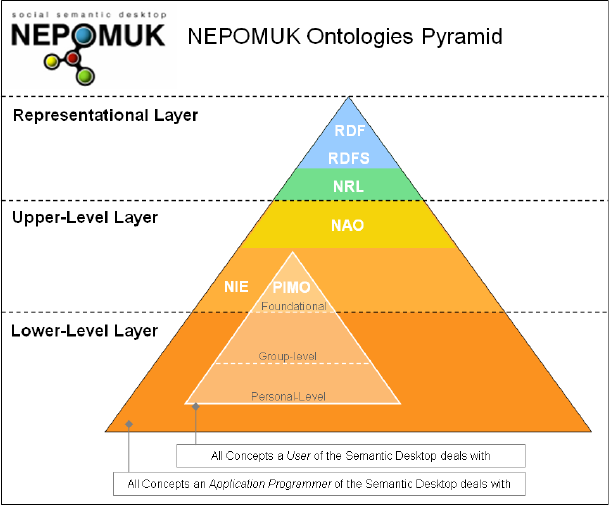
\includegraphics[width=0.8\linewidth]{chapters/background/img/ontologies.png}
\caption{The pyramid of desktop ontologies.}
\label{fig:ontologiespyramid}
\end{figure} 

To accommodate some restrictions specific to describing desktop and personal data, an extension to RDF was developed. It is called NEPOMUK Representational Language (NRL)\footnote{\url{http://oscaf.sourceforge.net/nrl.html}, previously at \url{http://www.semanticdesktop.org/ontologies/nrl}} \cite{Sintek2007}, and is a representational ontology, thus belonging in the top level of the pyramid. It adds Named Graphs and Graph Views to RDF/S and introduces the closed world assumption to the data. The named graphs in NRL are similar to the named graphs defined by \cite{Carroll2005} except that they do not follow the open world assumption. NRL defines graph roles for named graphs, where roles contain information about a graph's data and how it should be handled.

The open world assumption which is usually used on the Web, states that everything that is not known is undefined, which makes sense when working with very large amounts of information, most of it unknown. It does not work as well on the desktop, where we handle personal data that is implicitly known to the user in its entirety. That is why NRL introduces the closed world assumption, which states that everything that is unknown is false. However, NRL does not make any assumptions on the semantics of a graph defined with it. With the use of graph views over named graphs, there can possibly exist different views with different semantics over the same graph.

The upper level ontologies describe basic concepts generalising over multiple domains and activities specific to the desktop and PIM. There are three ontologies in this level: 
\begin{description}
 \item[NEPOMUK Annotation Ontology] (NAO\footnote{\url{http://oscaf.sourceforge.net/nao.html}, previously at \url{http://www.semanticdesktop.org/ontologies/nao/}}) contains concepts which allow users to annotate desktop resources, including custom descriptions, identifiers, tags and ratings. Generic relationships between related resources can be made explicit through properties defined in this ontology.
 \item[NEPOMUK Information Element Ontology] (NIE\footnote{\url{http://oscaf.sourceforge.net/nie.html}, previously at \url{http://www.semanticdesktop.org/ontologies/nie/}}) describes a unified vocabulary for native resources available on the desktop. NIE is in fact a larger framework, where the core part is the NIE ontology, complemented by several smaller vocabularies describing specific types of desktop resources, like files, music, emails, address book contacts, calendar entries, etc. Standards for representating many of these types already existed, either in the form of RFCs or in the form of Web vocabularies. In these cases, the existing resources were used as basis for the respective NEPOMUK ontologies. For example, the NEPOMUK Contact Ontology (NCO\footnote{\url{http://oscaf.sourceforge.net/nco.html}, previously at \url{http://www.semanticdesktop.org/ontologies/nco/}}) was designed based on the VCARD specification (RFC 2426 \cite{RFC2426}), and on the Vcard ontology\footnote{\url{http://www.w3.org/TR/
vcard-rdf/}}, but it has a much broader scope than either of the two. Similarly, the NEPOMUK Calendar Ontology (NCAL\footnote{\url{http://oscaf.sourceforge.net/ncal.html}, previously at \url{http://www.semanticdesktop.org/ontologies/ncal/}}) is an extended adaptation of the W3C calendaring ontology\footnote{\url{http://www.w3.org/2002/12/cal/}}. NIE defines two disjunct classes of resources, \verb|DataObject|s --- the physical representation, and \verb|InformationElement|s --- the interpretation and content of resources. The two are then subclassed in each specific vocabulary of the framework. The NIE classes are designed for machine use in extracting semantic information from existing desktop sources and applications, not for direct handling by the users.
 \item[Personal Information Model Ontology] (PIMO\footnote{\url{http://oscaf.sourceforge.net/pimo.html}, previously at \url{http://www.semanticdesktop.org/ontologies/pimo/}}) is both a upper level ontology and a lower level ontology, as it contains both generic concepts and quite specific ones. From a user's point of view, PIMO is the central ontology of the Semantic Desktop. Its scope is to model the data that the user works with. According to its specification \cite{Sauermann2009a}, ``PIMO is based on the idea that users have a mental model to categorize their environment'', and ``each concept in the environment \dots is represented as [a] Thing in the model''. PIMO defines high level types like Person, Project, Event and Task, which reflect the user's mental image of the objects, not their representation in various desktop applications, nor the files used to store the information about them. That is the task of the NIE ontology and framework, while the PIMO is needed to provide an aggregated view of all 
the possible sources of information about a \emph{thing} the user needs.
\end{description}

The lower level ontologies consist of domain ontologies and application ontologies --- which have very specific or limited use cases. 
Users can import new ontologies into their Semantic Desktop either directly or through applications. When certain ontologies become widely used, it is recommended that they go through a process of standardisation and are included in the desktop ontologies, in order to support reuse. 

Existing ontologies can be customised by users or by application developers, this is however discouraged for the upper level ontologies, as it would affect interoperability between Semantic Desktops.

\subsubsection{The NEPOMUK Reference Implementation}

The reference implementation of NEPOMUK is based on the blueprint defined within the project, but it is not an exact realisation of it. The general structure is maintained however, and several of the possible services are provided. The implementation is done in Java, for portability.

\begin{figure}[tb]
 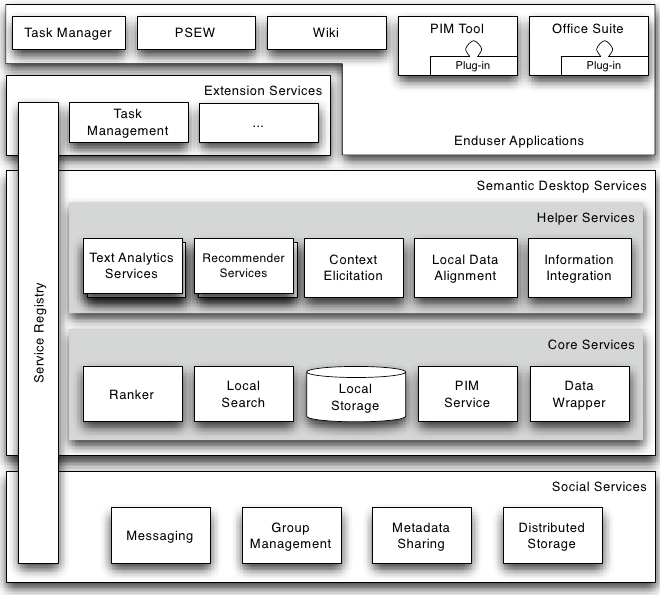
\includegraphics[width=0.8\linewidth]{chapters/background/img/javaarchitecture.png}
\caption{The architecture of the NEPOMUK Java implementation.}
\label{fig:nepomukjava}
\end{figure} 

The service oriented architecture of the Java implementation of NEPOMUK uses SOAP and OSGi for communications between the services, and for discovery. The component which provides the registry and discovery functionality is called the NepomukMiddleware (or Middleware), and it is a service itself. The implementation evolved from a local web server with SOAP, to Eclipse, as it has better support for inter-service communication.

Figure \ref{fig:nepomukjava} \cite{Reif2008} shows the services composing the reference implementation. The core services provide functionalities for extraction, storage, and retrieval of the semantic desktop data. They are fundamental for the functionality of the Semantic Desktop, as they are used by all the other helper services and applications built on top of the framework. 

The storage service is the central service of the Semantic Desktop. All the semantic data is stored and retrieved from here, thus acting as a blackboard (see Section \ref{sub:characteristicsofsd}). The storage service uses existing triple store implementations, current version using Sesame2. Additionally it provides some basic inference and query support. Lucene is used for indexing. 

The DataWrapper service extracts information from desktop sources and stores it in semantic form in the central RDF store. It uses plugins to access and extract data from application specific formats and repositories. Other helper services can be combined with the DataWrapper, to ensure that the data is well integrated and that duplicates are removed (e.g. an integration service), a data alignment service, or an inference service to extract new information based on the existing triples. 

The PIM service provides convenience methods to access and create information in a user's PIMO. 

The local search service provides search functionality over the local repository, supporting both structured queries and full text search. It includes the functionality provided by a Ranker service, which computes resource relevance for better search results. 

Additional helper services were developed: a Context service, Recommender services, Text Analytics services. 
On top of the core services and the helper services, several extension services were developed, to showcase possible uses and to demonstrate how the services can be combined. 
On top of the services, applications were built to provide functionality to the users in a friendly user interface. The interface to this implementation of the NEPOMUK Semantic Desktop is called PSEW (Personal Knowledge Workbench) \cite{Grimnes2009}. It offers a visual way of interacting with the services, as well as several views of the data contained in the local repository. Other specialised applications were developed: a semantic email extension \cite{Scerri2009} to Microsoft Outlook and to Mozilla Thunderbird, a plugin for Microsoft Word \cite{Groza2011} to semantically annotate documents, etc.

The social part of the Social Semantic Desktop was meant to be fully distributed, thus a P2P network implementation was used for the majority of the services. However, a centralised NepomukHub was developed as well, using XMPP. The NepomukHub acts as a server for inter [Semantic] Desktop communication, passing messages between NEPOMUK instances, and also as a shared triple store, where social information, like group memberships, is stored and managed. The messages sent through the NepomukHub transport RDF graphs, thus any semantic information can be shared among desktops. Several social services were developed on top of the P2P network and the NepomukHub infrastructure. They include a Messaging service, a Metadata Sharing service, a Distributed Storage service and Distributed Search. Local services can be extended to use the social services.

\subsubsection{Nepomuk-KDE}

By far the most successful part of the NEPOMUK project was the ``Mandriva Community scenario'' \cite{Lauriere2006} or Nepomuk-KDE\footnote{\url{http://nepomuk.kde.org}} as it became known. It was initially meant as a proof of concept, showing that the blueprint can be realised outside of the reference implementation. The start of the NEPOMUK project coincided roughly with the beginning of development on a new major version of the KDE\footnote{KDE has been rebranded in the mean time to refer to the community instead of the software produced. Thus KDE is no longer an acronym for ``K Desktop Environment''.} Desktop Environment for Linux --- KDE4. Thus it provided the opportunity of including the new research ideas into an emerging platform, more deeply than it could have been done for a system that was already completely designed and implemented. As a result, Nepomuk-KDE is part of the core libraries of KDE and is used in several central applications, the best example being Dolphin, the default file manager. 
Desktop search is also done through NEPOMUK, and metadata creation, such as tagging, rating and commenting, is available desktop-wide. The adoption of NEPOMUK and semantic technologies has been very good, and development on the framework continued after the end of the EU project, driven by the community that was formed.

Including NEPOMUK in KDE also meant convincing the developers of KDE applications to make their software use the new semantic features. It required familiarising them with the semantic technologies used, and encouraging them to participate in the development of the framework and to collaborate on the ontologies. 

For open source projects like KDE, there are restrictions on what libraries can be reused due to software licences. This had an effect in the first stages, on the fact that the Java code of the NEPOMUK reference implementation could not be directly reused. Although it is possible to run Java on Linux, there are restrictions on the distribution of Java libraries. That was one of the reasons why Qt, the language in which KDE is developed, was preferred for Nepomuk-KDE. Although it is possible to use Java libraries in applications, code written in Qt/C++ was preferred by the packagers of the distributions that used KDE4. Thus, despite inferior results and features, many Nepomuk-KDE Semantic Desktops used the Redland\footnote{\url{http://librdf.org/}} C library for the storage service, while at the same time Sesame2 library was available but since it was written in Java, it required additional configuration. Currently Nepomuk-KDE uses a customised trimmed down version of OpenLink's Virtuoso\footnote{\url{http://
virtuoso.openlinksw.com/}}. It is feature-rich, stable, and the close collaboration with the OpenLink developers resulted in a version tailored specifically for running a triple store on a desktop.

Architecture-wise Nepomuk-KDE differs from the blueprint. For simplicity the social part has been ignored in the start, and the focus was on providing easy and simple to use semantic features to attract more contributors before diving into more complex tasks. Several social aspects are being implemented now with the use of NEPOMUK in the Telepathy\footnote{\url{http://telepathy.freedesktop.org/}} project.

The services in Nepomuk-KDE are also different. The preferred inter-service communication method is either through DBus\footnote{\url{http://www.freedesktop.org/wiki/Software/dbus}} or API calls. The services themselves are not defined as Web services running on the desktop, but as KDE modules. They are managed through a NepomukServer service.
As already mentioned, the current implementation of the Storage service uses Virtuoso as the default triple store, although other backends can be configured for use. 
The Data Wrapper function is done by Strigi\footnote{\url{http://strigi.sourceforge.net/}}, but instead of independent plugins for external applications, Strigi is a plugin-based system, with each plugin being responsible for certain types of files. Other exporters of semantic data come from Akonadi\footnote{\url{http://community.kde.org/KDE_PIM/Akonadi}}, the PIM framework of KDE.

The Nepomuk-KDE framework is changing continuously, due to the active community around it. It is evolving together with KDE and because of it, the uptake has been considerable, with many developers adding semantic features to their applications, and thus increasing the visibility and attracting more users.


\subsection{Characteristics of Semantic Desktops}
\label{sub:characteristicsofsd}

\subsubsection{Architecture}
\label{sub:architecture}

Most of the systems described in Section \ref{sec:sdsystems}, along with NEPOMUK, agree on the need for a layered architecture for Semantic Desktops. The layered general architecture shares many common points with the conceptual architecture for applications on the Web of Data, as surveyed in \cite{Heitmann2012}.
It can be divided into three major layers which build on top of each other, with dependencies and even overlaps between them.

\begin{description}
 \item[Data layer] The Semantic Desktop revolves around the [semantic] data that it contains. As such, the architecture is also centred around handling this data. This layer contains the vocabularies for describing the data, and the data itself. 
 \item[Service layer] Based on the data, the Semantic Desktop provides an enabling framework of basic services, which can be either visible or transparent to users. This framework enables the functionalities of the applications. The set of basic services vary among the systems described, but are indispensable to them. These services are central to the desktop, and generally accessible from all applications. Some of the basic services include storage, extraction, integration, query, inference, annotation. 
\begin{description}
 \item[Storage service] can vary from a database system like MS SQL server used by MyLifeBits, to a fully fledged RDF store like Sesame or Virtuoso in Gnowsis and NEPOMUK. Many systems use Jena (SEMEX, IRIS) and some use files. Some use a combination of storage from the options above (MOSE has three --- database, file and Jena RDF store). Depending on the type of storage, semantic resources are identified either by URIs or by unique database IDs. 
 \item[Extraction service] can come under several names --- crawlers, wrappers, gatherers --- however, they provide the same function, that of extracting semantic information from non-semantic sources, whether structured or unstructured. It can vary from simple extractors of metadata already available for files --- like photos (EXIF) and music (ID3), or emails --- sender, subject, to parsing and analysing unstructured text to extract information from multiple file formats (Stuff I've Seen, SEMEX, Gnowsis, NEPOMUK). CALO features natural language analysis to extract entities and relations among them. MOSE also extracts resources and relations from files, and stores two types of information --- R-F links, which specify which resource was extracted from which file, and R-R links, which specify connections between resources. Semantic information extraction plays a significant role in providing the basic functions of a Semantic Desktop, and all the systems described here implement it. The extraction service 
generally comes bundled together with an instance matching service.
 \item[Integration service] (instance matching, entity matching, or de-duplication) has the role of checking if two instances are the same. The definition of \emph{the same} varies from system to system. One of the main uses of this service is complementing the functionality of the extraction service, by checking if a newly extracted entity already exists, in which case, depending on the policies the existing entity is reused instead of creating a copy, or a new entity is created and linked to the existing one.
 \item[Query service] All the systems allow querying their semantic data. Keyword search is supported by IRIS, Semex, Haystack, and MOSE. For keyword search, an \textbf{indexing service} is used, which can be an independent service, or part of the storage or the extraction service. Structured query languages like RDQL and SPARQL are also supported in MOSE, IRIS, Gnowsis, X-COSIM, and NEPOMUK. The ways in which the results are displayed are discussed in the presentation layer. 
 \item[Inference service] Inference on the semantic data is supported by IRIS, Gnowsis and NEPOMUK. This service can be standalone or included in the extraction or the integration service. The quality of the inference results depends on the engine used and the ontologies used to describe the data. 
 \item[Annotation service] All systems allow some type of annotation of resources, however, not always in the form of a standalone service. Annotation refers to creation of metadata for resources, or of new connections between resources. Manual creation of new resources can also be considered annotation. Some automatic annotation is performed by the extraction and the integration services. In Haystack, where there is one access point to the data, the annotation service is in fact a user application, as it happens directly. In MyLifeBits annotations play a central part -- the system allows sharing, annotation of annotations. The most basic types of annotations are tagging and grouping in collections, which are both used for categorisation.
\end{description}
\item[Presentation / Application layer] The user-facing interface of the Semantic Desktop makes up the presentation layer, built on top of the supporting framework. The systems have a large variety of user interfaces, providing functionality that varies from simple resource browsers, to complex PIM tools like email clients and task managers. 
\end{description}

Regarding the applications they provide, the systems are divided in two categories, depending on whether they choose to enhance existing applications with semantic capabilities, or propose new semantically enabled applications to replace existing ones for PIM tasks. X-COSIM, Gnowsis and NEPOMUK belong to the first category, while IRIS and MOSE belong to the second.

The flexible and customisable visualisation of information is one of the distinguishing features of Haystack. It is a Semantic Web browser \cite{Quan2004}, providing a unified interface for the data it contains, with the added functionality of allowing edits \cite{Quan2003b} and customisations. The feature that sets Haystack apart from other semantic browsers is its dynamic creation of user interfaces. This is realised by recursively rendering semantic resources \cite{Huynh2003,Karger2005}. The way an object should be rendered is described in RDF. General visualisations are provided out of the box, but users can customise them according to their needs. 

Most systems provide a resource browser and search interface in the style of Haystack, although usually not as flexible. Some browsers display the underlying ontology. They allow changes to be made to the data directly through this interface. 
Faceted browsing and browsing by association are available in all resource browsers.

MyLifeBits and SEMEX propose that multiple visualisations be supported for resources, depending on the user's context.

\subsubsection{Blackboard and fuzzy layers}

The layers of the architecture can overlap.
The storage service is at the fuzzy border between the data layer and the service layer. It is responsible for the persistent storage of the data and for providing low level access to it. Since the storage service is highly connected with the data, it can be seen as part of the data layer, but at the same time it is a foundational service, and as such it is part of the service layer.

Similarly, services which provide any type of user interfaces are at the border between the service layer and the presentation layer.

Inside the service layer itself we can see a separation based on the level at which the services operate. Some foundation services are more oriented towards the data - like an inference service or the analyser and extractor services. Other services provide more user-oriented functionality, like an annotation service, or a query service. 

Services can use functionality provided by other services, communicating and building on top of each other. The communication between the services, as well as the communication between the services and applications can take several forms: through programming interfaces (APIs provided by the framework), Web standards (Gnowsis promotes a Web server as a desktop service), or P2P communication (MOSE, NEPOMUK).

The architecture of many of the systems uses the Blackboard pattern, where the blackboard is the data storage, or even the entire data layer, which is accessible to all services and applications. They have the role of the specialists in the pattern. The control element is the storage service. Specialists populate the blackboard with data which can then be accessed and refined by other specialists. For example, a PDF extractor service can parse documents and extract titles, authors and affiliations. The data must then be processed by the integration services, so that duplicate authors and affiliations can be merged into a single unique representation. Furthermore, the inference service can then extract co-working relations between the people, based on common affiliations.

\subsubsection{Data Representation}
\label{sub:vocabs}

Semantic data is the most important part of the frameworks, and the way it is described influences the quality and quantity of things that can be done with it.

All the systems define a data model for the data they use and extract. The data models vary from very small and generic, like the one in SEMEX, which has a restricted number of classes and associations, to the comprehensive one provided by X-COSIM.

Being small, SEMEX's ontology is unitary, but the bigger ones usually are modular. MOSE's ontology is divided in small application ontologies belonging to the PIAs and domain ontologies used by the services. CALO also has different ontologies for specific domains and used by specialised agents. X-COSIMO is divided into modules representing different aspects of the data.
More than being modular, the set of ontologies used by NEPOMUK is also layered. The representational level defines the vocabulary used to define the other ontologies. The upper-level ontologies contain domain-independent abstract knowledge. The lower level ontologies contain specialised concrete terms from the user's mental model. The low level PIMO plays an important role in both Gnowsis and NEPOMUK, as it is used to describe the data most often handled by the user.

Most of the frameworks use RDF or OWL ontologies to describe the data.
Only MyLifeBits and SIS do not mention the use of ontologies, MyLifeBits using a flexible database schema to define the data model. 

Another differentiating characteristic is whether or not the data model can be personalised by the users by creating new types and new relations. X-COSIM does not allow the modification of the domain ontology, but it does allow the creation of custom mappings from and to other external ontologies. Haystack and SEMEX on the other hand argue for the need for personalisation of the ontologies by the user, as only in this way, can a truly personal mental model be created. Most systems do support the customisation of the underlying model, as well as the import of new vocabularies in the system, by linking to them or through mappings. This fact raises the challenge of reconciling data described with customised models. 

The long-term study by \cite{Sauermann2008} found that very detailed ontologies are not necessarily more useful for the users, as simpler and more generic relations are preferred over more specific ones. The intuition is that the more precise properties, although better at classification, present the added challenge of choosing the suitable one. 
The same study of using Gnowsis has shown that although customisation of the underlying ontologies is supported, the users only make minimal and rare changes. This result confirms the MyLifeBits hypothesis that although their schema is flexible and can be modified, users will probably not make any changes to it. While a layered system like NEPOMUK's gives more flexibility, allowing users to change and update the ontologies gives too much flexibility for the normal use cases, and would be used only by a few power users, in a very limited number of occasions. Most customisations were sub-classing existing classes and specialising existing properties by creating sub-properties. 


\subsection{Discussion}

In this section we covered some common aspects of the systems regarding their architecture, the functionalities they provide and the way they represent and work with data.
Following again the layered structure used before, we continue with a discussion of some of the shortcomings and possible developments which appear to affect all or most of the Semantic Desktops. 

At the data level, as the systems have evolved, the ontologies they employ have become more complex. While providing good coverage of the PIM domain, comprehensive vocabularies with detailed relationships among types showed that the simpler, more general relations are used much more often, regardless of the possible loss of meaning \cite{Sauermann2008}. Hence, rich ontologies are not necessarily better, since most users prefer simple relations between resources, which are enough to remind them of the connection, without specifying it fully. Detailed vocabularies might prove more useful in the case of automatic processing of data, but using them to manually annotate is costly.

Moving into the service layer, the storage and the indexing services provided by the systems use semantic technologies which have evolved at a rapid pace. A slow repository, and thus slow response times for queries and browsing have at least partially been at fault for the poor uptake of the Semantic Desktops. Fast and memory efficient triple stores are now available.

Regarding the applications provided by the systems, we observed the distinction between integrating semantics into existing applications versus creating new semantic applications. 
Forcing the users to switch from the applications they know to avail of the power of the Semantic Desktop in applications they would need to learn how to use, has not proved to be a successful strategy. However, systems like Gnowsis, X-COSIM and NEPOMUK use plugins to add semantic functionality to existing popular tools, thus letting users continue to use their preferred tools while benefiting from the added semantics.

One of the reasons for the slow uptake of the Semantic Desktop could be the cold start problem, which is observable despite multiple automatic ways of extracting, linking and importing resources, and kick-starting the system. This could prove that the user's manual annotations are more important than the automatically extracted data, which has its own important role though. However, since the automated data comes from sources which are accessible to the user anyway through conventional tools, there is no immediate incentive to use the semantic applications, which translates in little manual information being added into the system, and the benefits delayed further, despite several evaluations \cite{Franz2007,Sauermann2008} proving that Semantic Desktops \emph{are} better for PIM tasks \cite{Franz2009}.

It could also be that the visualisations used for the automatically extracted data are not suitable for the purpose, or not attractive enough.
Generic graph or table visualisations are not appealing, and treating every resource the same is not an effective way of conveying information.

In recent years two developments occurred and influenced the direction in which the Semantic Desktops evolve: \begin{inparaenum}[(i)] \item the exponential growth of semantic data available online, mostly due to the Linked Data initiative and the Linking Open Data project which have a large success, and \item the growing concern about the privacy and security of personal data\end{inparaenum}. 
Some of the information available as Linked Data might be relevant to the users of Semantic Desktops, so using it in applications and services to add value to the users is a low hanging fruit, -waiting to be picked. However, the open aspect of most of the available data causes concern especially when it becomes mixed with valuable private personal information. Privacy is not the only concern, albeit a very important one. Establishing whether the Web information is trustworthy is another concern, and possibly a harder one to tackle.

\section{Conclusion}

This chapter covered Semantic Desktop systems and applications described in literature, starting from the historical ones like the Memex, NLS and Xanadu, to recent ones like NEPOMUK. We showed that they share common goals and characteristics, and we extracted and discussed their general architecture and data representation means. Understanding these is very important for the core part of the thesis, as our work is grounded and builds on top of the framework provided by the Semantic Desktop, specifically, the Nepomuk-KDE Semantic Desktop.

In recent years other systems have emerged, targeting the issues described above, on the desktop or other devices, by using semantic technologies. However, the focus has changed from exploring possible architectures and creating vocabularies, to a more data centric approach. The Semantic Desktop has matured, along with the semantic technologies it employs, so that now new and more exciting, as well as harder, problems arise. Now that the infrastructure has been put in place, the Semantic Desktop awaits the killer app which would bring it and the possibilities it opens into the public eye. Siri\footnote{\url{http://www.apple.com/iphone/features/siri.html}} and Evi\footnote{\url{http://www.evi.com}}, as well as IBM's Watson\footnote{\url{http://www-03.ibm.com/innovation/us/watson/}} have led the way.

In the next part, we continue by presenting the core research of the thesis, which builds on top of the base set by the Semantic Desktop, to better interlink personal information, not only within the desktop, but also to the Web.


 \part{Core}
\label{part:core}

In the core part of the thesis we present o-ur main contribution, consisting of research and applications towards better interlinking of information on the Semantic Desktop. We introduce interlinking of personal notes with the semantic note-taking tool SemNotes, then we present a method for connecting Semantic Desktop data to the Web of Data, followed by the description of a use case and system for semantic publishing which incorporates and builds on the two previous chapters. Each of the chapters is based on previously published works.

We start from the premise of the Semantic Desktop --- it provides the framework we need for building our network of linked personal information. The order of the chapters follows the logical order of interconnecting Semantic Desktop information. 

We start at a local level in Chapter \ref{ch:semnotes}, by describing ways of creating new semantic data within the desktop, integrating it with the existing information from the desktop, and making it accessible across application borders. In this context, we present the challenges we found and our solutions to semantic application development on the Semantic Desktop.

Since the personal information we use is no longer restricted to the desktop, it has become important to expand the network of personal linked data beyond the desktop, into the Web of Data. Making use of the large amount of data available online in linked form, in Chapter \ref{ch:sdwod} we describe a method for bridging the gap between the two linked data networks --- the Semantic Desktop and the Web of Data. 

In Chapter \ref{ch:semblogging} we merge the interlinking of new notes with existing semantic desktop data from Chapter \ref{ch:semnotes} with the interlinking of the same data with Semantic Web from Chapter \ref{ch:sdwod}, for the purpose of semantic publishing. The solution we present is not limited to the use case of semantic blogging, but it is valid also for e-health use cases like patient records and doctor notes, or for the enterprise domain, for reporting or collaboration. 

In the last chapter of the section, Chapter \ref{ch:mischelperapps}, we describe several other proof of concept applications we developed with the same goal of enabling and supporting better interlinking of personal data on the desktop and beyond. 

The work builds on top of the Nepomuk-KDE branch of the NEPOMUK Social Semantic Desktop, described in detail in Section \ref{sub:nepomuk} and it reuses the ontologies defined within the NEPOMUK project. Using the libraries and vocabularies in an application has led, as a collateral result, to improvements and changes in both.


\chapter
{Creating and Interlinking Semantic Data on the Desktop with SemNotes}
\label{ch:semnotes}

\begin{flushright}
 \textit{Based on ``The Semantic Desktop at Work: Interlinking Notes'' \cite{Dragan2011a}\\published at the 7th International Conference on Semantic Systems (I-SEMANTICS~2011)}
\end{flushright}

The Semantic Desktop has been proposed as a solution to the ever growing problem of information overload on our computers. It provides the foundations necessary to integrate and manage personal information. However, the challenge of designing and realising semantic applications that use this infrastructure still remains. 
In this chapter, we present SemNotes\footnote{\url{http://smile.deri.ie/projects/semn}}, a semantic note-taking tool for the Nepomuk-KDE Semantic Desktop, as a tool for creating new semantic information on the desktop and integrating it seamlessly in the existing network of linked desktop data.
SemNotes provides a real-world, functional use case for fully exploiting the capabilities of the Semantic Desktop: interlinking, organisation and management of personal information, improved search and browsing. 
Furthermore, it represents our solution to a set of identified generic challenges for applications on the Semantic Desktop, as described by the first research question in Section \ref{sub:question}.
We describe a task-based user evaluation comparing SemNotes with a conventional note-taking tool. The results show that complex searches on interlinked information created with SemNotes are significantly faster, with little or no extra effort required from the users. 

\section{Introduction}
\label{sec:semnotesintro}

The Semantic Desktop provides a framework for creating applications and tools that simplify the daunting tasks of managing personal information accumulated on the desktop. 
The information overload problem, combined with the disconnection of data caused by application silos, is solved by the use of Semantic Web standards for storing and interlinking the desktop information. 
Data which before was stored separately by different applications can be now explicitly connected. The result is a network of interlinked personal information, which can be browsed by association, filtered and searched in a unified way. 

The Semantic Desktop overcomes the limitations of conventional desktops, where information is kept in different formats and application repositories, by using common vocabularies to describe the data, and a desktop-central place to store it, in a standardised format, accessible to all applications.

Indeed, the Semantic Desktop makes the information load manageable. However, new challenges emerge: one such new issue is how to design and realise semantic applications that use the infrastructure provided by the Semantic Desktop. We address this problem by dividing it into smaller, simpler challenges and providing solutions for each of them. To illustrate the solutions, we describe the design of a semantic note-taking application for the Nepomuk-KDE Semantic Desktop, called SemNotes. We use note-taking as an example because it is a desktop activity that is not limited to a specific domain, since the notes can widely vary in topic. It is also a common activity that plays an important role in Personal Information Management and that we believe would benefit from the use of semantic technologies.

\subsection{Challenges}
\label{sub:appchallenges}

In Section \ref{sub:question} we broke down the first research question \textbf{Q 1.}: \emph{How to build semantic applications and tools for the Semantic Desktop as to provide the best experience for the users, while creating reusable semantic data?}, into several sub-questions.
These are the challenges we found in designing new semantic applications for the Semantic Desktop:

\begin{description}
 \item[Q 1.1.] \emph{How to create semantic data that is correct, and maximises the reuse of existing Semantic Desktop data through interlinking?}\\
Applications should be aware of the data that is available on the desktop, from other applications. The data they produce is also accessible to other applications, and this should also be taken into account, because it raises the dual challenge of making sure that the data is represented correctly so that other applications can use it if they choose, as well as making the most of existing information through reuse and link creation. How to interlink information items is the most important challenge for adhering to the Semantic Desktop requirements of creating and maintaining a network of linked desktop data. It refers in the first place to the new information coming into the desktop through the application, and how to integrate it with the linked information that exists on the desktop. But it also covers the situation when the only new information created is in fact a new link between existing entities. 
Existing desktop data is heterogeneous. The reasons for this include the fact that different parts of it are created by different applications, with different functionalities and needs. So, although represented in a standardised way, the data is not always consistent, up-to-date or even correct. Furthermore, the data is also heterogeneous in terms of form: there are new types of information available to be integrated (i.e. tags, relations). Best practices advise the reuse of as much of the existing information as possible, because through reuse, the interlinking becomes deeper and richer. However, the possibility of reusing vast amounts of existing data raises other challenges, in selecting the right amount of necessary information for maximum benefit for the users, while not overloading them. The selection is complemented by the way the information is shown.
 \item[Q 1.2.] \emph{How to design the human-computer interaction in an application for the Semantic Desktop?}\\
This question relates to designing interfaces which support the existing workflow of the user, while integrating the additional semantic information in a useful way. A balance must be found between too much information, so that it interferes with the user doing tasks, and too little, or not enough to make a difference. The question also refers to more than just displaying the information in an interface --- allowing users to interlink information items easily, and generally aiding the creation of new semantic data is also a challenge for application development. Extra difficulty is added by the variety of interlinked information available on the desktop, combined with the reduced control of developers over what resources are linked from other tools.
 \item[Q 1.3.] \emph{How to correctly evaluate a semantic application?}\\
A challenge related to evaluation is the lack of a standardised dataset to use, due to the highly personal data required. Even if such a dataset existed, due to the fact that the applications on the Semantic Desktop are mainly related to personal information, it is difficult for participants to use the data provided, as they are not familiar with it. Evaluating PIM tools has been shown to yield best results when the test users are asked to perform their own tasks in their own set-up rather than attempting to simulate it with artificial tasks and artificial data. The reduced number of semantic application in each area makes it difficult to evaluate a new tool against an existing established one, thus the best candidates for a comparative evaluation are conventional (i.e. not semantic) applications with similar functionality. While possibly re-demonstrating that indeed linked data is more useful, comparing a semantic and non-semantic application requires well thought metrics, as the semantic features that need 
evaluating have no direct counterparts against which to evaluate them. For task based evaluations, it is difficult to find a common set of tasks that both applications can perform. A solution is to choose general, high level tasks, but that influences the granularity of the results.
\end{description}


\section{Tackling the Challenges: The Design of SemNotes}
\label{sec:semnotesdesign}

We use our note-taking application, SemNotes, to describe the general principles we used for designing an application for the Semantic Desktop. Note-taking is a good general use case for the Semantic Desktop because the information contained in notes is not restricted to a specific domain. Personal notes are naturally connected to the user's context, and can thus be meaningfully interconnected with much of the existing network of personal data on the desktop.

We divided the design into specialised modules. Each module handles a set of related tasks. We describe the modules as they would be for a general semantic application, followed by a more specific description about the implementation of SemNotes in the next section.
 
\subsection{Data Representation} 

This module handles the vocabulary of the application: the \emph{data types} around which the application is centred, and the kind of \emph{metadata} that is needed for them. To enable other Semantic Desktop applications to understand the data produced, as well as for our application to understand data from the underlying Semantic Desktop, the best practice is to reuse existing desktop ontologies where possible. The basic data type handled by SemNotes is the note, represented by a short snippet of text containing personal information. 

\subsection{Data Management} 

This module manages the life-cycle of the semantic data that the application handles, by enabling the transition between the phases of the life-cycle. We adapted the Abstract Data Life-Cycle Model \cite{MoellerPhDThesis2009} to illustrate a comprehensive workflow for Semantic Desktop data, from its creation to its termination. Figure~\ref{fig:datalifecycle} shows the phases and transitions between them, focusing on the possible actions that the user can execute, and hence, that a semantic application could support.

\begin{figure}[htb]
 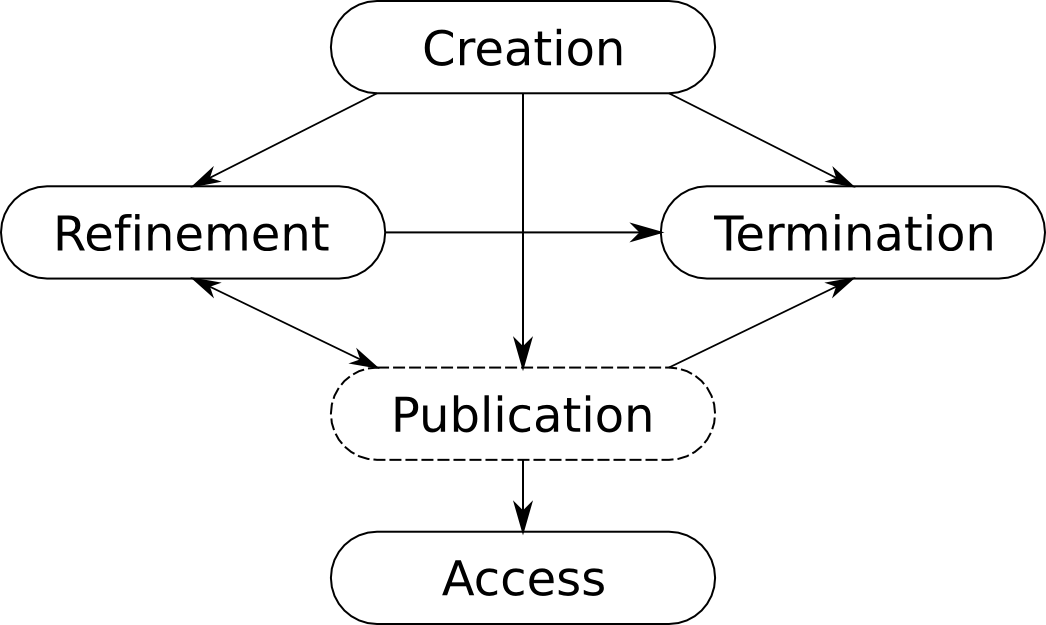
\includegraphics[width=0.7\linewidth]{chapters/core/img/lifecycle}
\caption{Semantic Desktop data life-cycle.}
\label{fig:datalifecycle}
\end{figure} 

\begin{description}
 \item[Creation.] Most often creation implies creating a new resource, of a given type. However, the import of existing data from other applications or formats (e.g. crawlers) is also included here.
 \item[Refinement.] This phase includes any activities that make changes to existing data. It also contains the creation and deletion of links between existing resources, although alternatively they can be included in the Creation or Termination phases, as links are data too. 
 \item[Access.] This phase is represented by accessing the data through either querying or browsing. Because we are discussing interlinked data, accessing a piece of semantic data implies recursively accessing the sub-graph of resources semantically related to it. How much of the sub-graph is traversed can vary, and further traversal by the user should be supported and encouraged. 
 \item[Termination.] In this phase the data is deleted from the system. As with the access phase, rules must be defined to determine how much of the dataset a deletion will affect---e.g. it might make sense to delete all the subtasks of a task when the parent is deleted, but not to delete the documents related to the task.
 \item[Publication.] This phase represents making the data accessible to users from outside the system. Also included here is exporting the data to other formats and applications. When handling semantic personal data, applications should ensure that sensitive data is well protected against unauthorised or accidental publication. 
\end{description}

Furthermore, this module handles where and how the data is stored. The Semantic Desktop provides the framework for storing semantic data, therefore it is best that the central desktop repository be used, when practical. This enables easier interlinking with the rest of the data. In the case of SemNotes, the notes and all the metadata about them are stored in the desktop repository. 

\subsection{Interlinking} 

The interlinking module is logically a sub-module of the Data management one, as it specifically manages a part of the refinement phase of the data life-cycle. However, because it is an important part of any semantic application, relating to the first two challenges listed in Section \ref{sub:appchallenges}, we describe it as a standalone module. The interlinking module effectively realises the goal of integrating the new semantic data into the pool of existing linked desktop data. The functionalities offered can vary from simple automatic linking of new resources to a specified context or to their author, to complex extraction and inference of new relations and resources.  This module provides the feature that sets SemNotes apart from other note-taking tools, the interlinking of the notes with the desktop resources mentioned in them. In our application, there are two sub-modules, that handle \begin{inparaenum}[(i)] \item entity recognition, and \item information extraction\end{inparaenum}, suggesting 
possible new connections to be created by the user.
 
\subsection{Visualisation} 

The visualisation module presents the data to the user in a simple, yet useful and versatile way. It addresses the third challenge listed above: designing the interface. Depending on the application, the visualisation can include \emph{aggregated} views on the data, and \emph{filters}. Faceted search \cite{Yee2003} has proven useful for semantic data, and it can be used to present the interlinked information to the user in a meaningful way. In SemNotes, the data that needs to be visualised is basically an enhanced version of a list of notes, with sorting and filtering. The module also provides the note editor. An important part of the module is displaying the recommendations for interlinking, a difficult task due to the heterogeneous nature of the information to be presented in a uniform, uncluttered way.

We describe how we tackled the last question --- the evaluation of the application --- in Section \ref{sec:semnotesevaluation}. 


\section{Implementation of SemNotes}
\label{sec:semnotesimplementation}

In the development of SemNotes, we tried to reuse as much as possible of the features provided by the host Semantic Desktop, Nepomuk-KDE\@. Using the existing functionality enabled better integration with the rest of the system, while reducing the effort required for the implementation. Nepomuk-KDE provides out of the box central RDF storage for the desktop, and an efficient means to access and query the data. 

We describe below the implementation of each of the modules introduced in the design section. 

\subsection{Data Representation} 
\label{sub:datarepresentation}

We describe the data created by SemNotes using a subset of the desktop ontologies described in Section \ref{sub:nepomuk} --- Personal Information Model (PIMO) and Nepomuk Annotation Ontology (NAO). 
Figure~\ref{fig:holiday} shows a basic note with metadata, and Listing \ref{lst:noterdf} contains the Turtle representation of the same example. 

The central unit of information handled by SemNotes is the note --- represented as an instance of \verb|pimo:Note|. 
The information stored for each note consists of: 
\begin{itemize}
 \item title --- \verb|nao:prefLabel|
 \item content --- \verb|nao:description|
 \item creation date --- \verb|nao:created|
 \item last modification date --- \verb|nao:lastModified|
 \item rating --- \verb|nao:numericRating|
 \item tags --- \verb|nao:hasTag|
 \item related desktop resources --- \verb|pimo:isRelated|
\end{itemize}

The Nepomuk ontologies make the distinction between resources representing native computer structures, which are described with the Nepomuk Information Element (NIE) ontology and resources representing concepts in the real world, which are described with the Personal Information Model (PIMO).

Before representing the PIMO concepts, most of the semantic data on the desktop is extracted from \verb|nie:DataObject|s and interpreted as \verb|nie:InformationElement|s. This is due to the fact that generally the information is still created by non-semantic applications, and to make it useful to the Semantic Desktop it has to be transformed, while keeping provenance information and feeding back into the applications that created it.

The extra step of extracting resources is not needed in the case of the information created directly for the Semantic Desktop by semantic applications. Thus, if no data is stored outside of the repository, no NIE resources are created. This is a characteristic of SemNotes and of other semantic applications for the Semantic Desktop.

The \verb|pimo:Note|s created with SemNotes can however be exported as text or HTML files, for backup or other purposes, thus associating a NIE resource to a note. This is the reverse of the usual process, and the change stems from working directly with the framework provided by the Semantic Desktop.

\begin{figure}[th]
 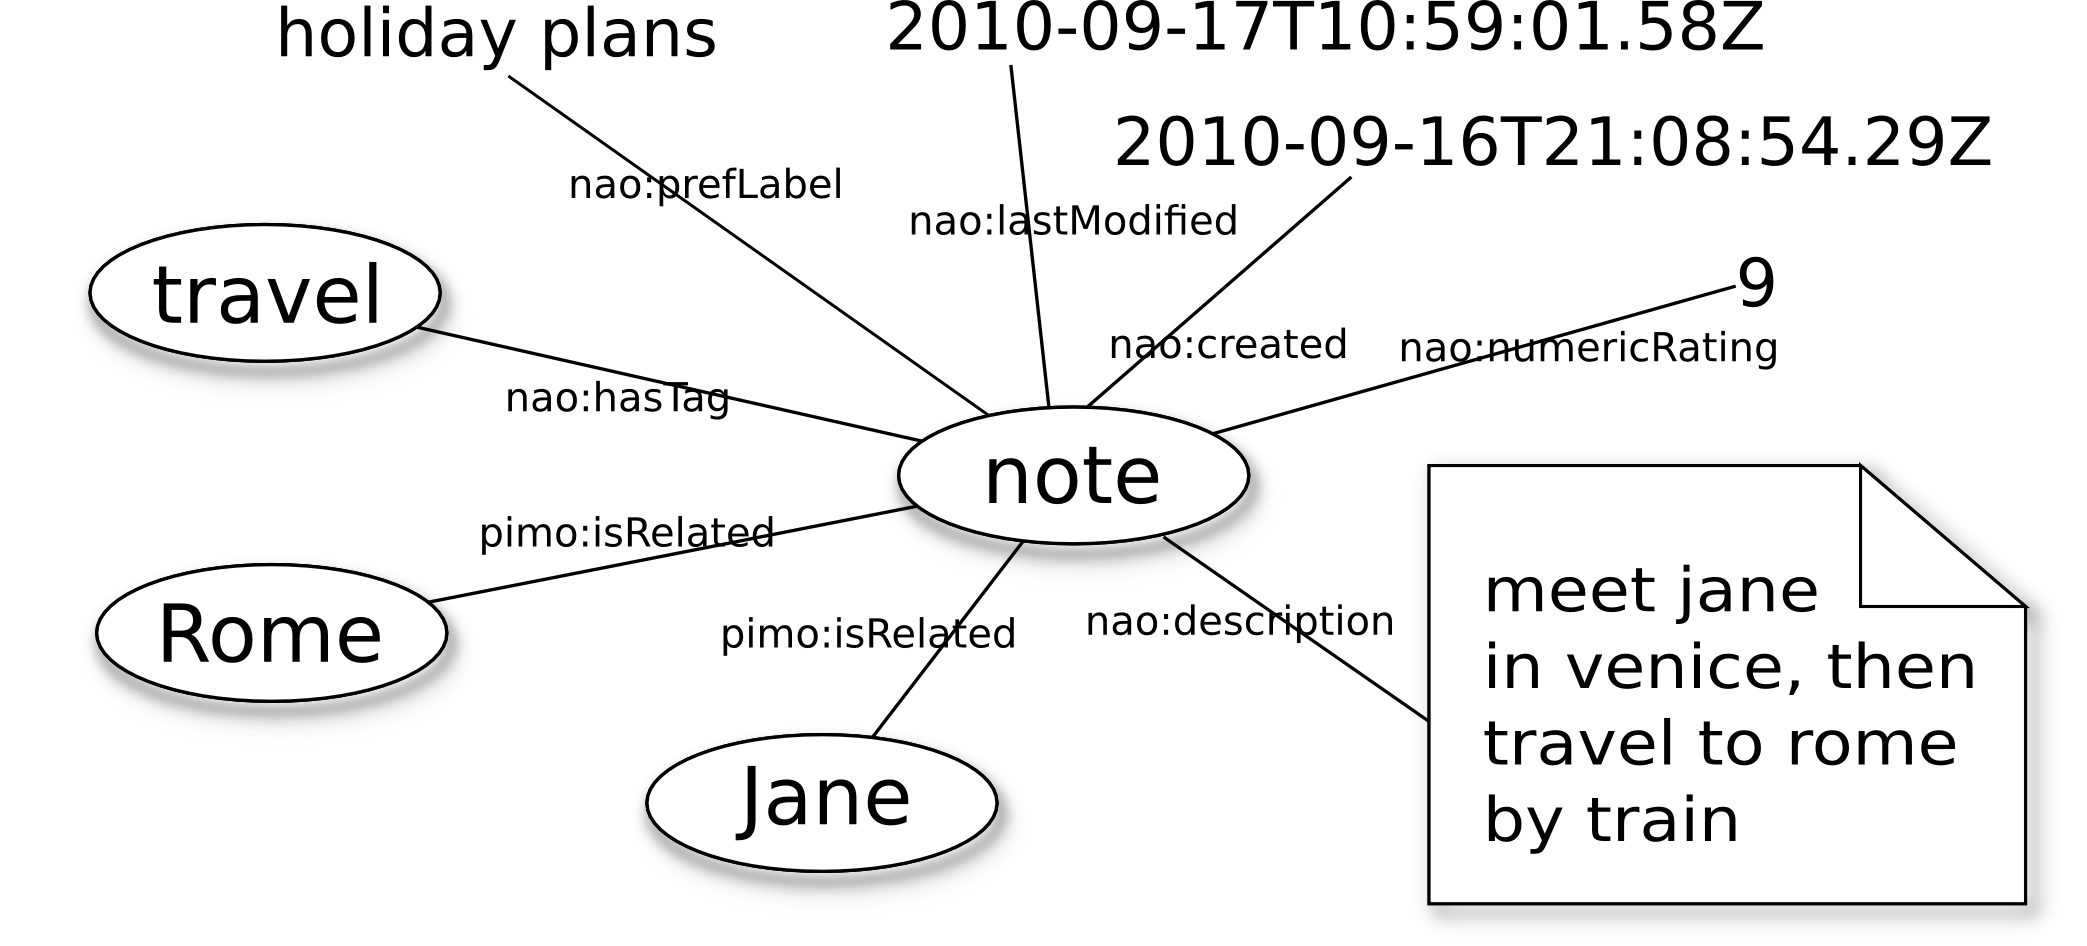
\includegraphics[width=0.9\linewidth]{chapters/core/img/note-properties}
\caption{Graph representation of the information about a note.}
\label{fig:holiday}
\end{figure} 

\subsubsection{Note metadata}

Tagging, rating and commenting are basic features provided out of the box by the Nepomuk-KDE system, for all types of resources. 
In SemNotes the only categorisation mechanism we use are tags, preferring simplicity over the more accurate mix of categories, topics and tags. The \verb|nao:hasTag| relation links the note to system-wide tag instances, thus enabling the reuse of tags throughout all applications, reducing duplication of classification work for the user. 

We later added support for rating to the interface, leaving the meaning of the rating open for the user to decide --- some possible examples include importance, urgency, quality of the content, or readiness for publication (in the case of a draft blog post as will be shown in Chapter \ref{ch:mischelperapps}).

Commenting on notes, although supported by the underlying system, because notes are resources, is not supported in the interface of SemNotes. We made this decision because the notes are themselves a type of comment, and we considered the feature redundant. 

\lstset{
	caption={RDF representation of a note.}, 
	label=lst:noterdf,
	language=turtle
}
\setlength\parindent{0in}
\begin{minipage}[t]{\linewidth}
\begin{lstlisting}
@prefix xsd: <http://www.w3.org/2001/XMLSchema#> .
@prefix pimo: <http://www.semanticdesktop.org/ontologies/2007/11/01/pimo#> .
@prefix nao: <http://www.semanticdesktop.org/ontologies/2007/08/15/nao#> .

<nepomuk:/res/thenoteuri> a pimo:Note ;
       nao:prefLabel "holiday plans"^^xsd:string ;
       nao:description "<html>...</html>"^^xsd:string ;
       nao:created "2010-09-16T21:08:54.29Z"^^xsd:dateTime ;
       nao:lastModified "2010-09-17T10:59:01.58Z"^^xsd:dateTime ;
       nao:numericRating "9"^^xsd:int ;
       nao:hasTag <nepomuk:/res/travel> ;
       pimo:isRelated <nepomuk:/res/Rome>, <nepomuk:/res/Jane> .
\end{lstlisting}
\end{minipage}
\setlength\parindent{0.21in}

\subsubsection{Note content}

Because notes are generally short \cite{Bernstein2008} we decided to store the note content in the RDF repository, as a property of the note (\verb|nao:description|). The value is the HTML string representing the content of the note, including formatting. This decision enables us to use the indexing and full text search feature provided by Nepomuk-KDE. 

Using the general property \verb|nao:description| to store the content of the notes, opens up the possibility of treating any semantic resource on the desktop as a note in SemNotes. This is equivalent to adding comments on each resource, but employing the functionalities provided by the application, including the analysis of the text to suggest relations. This enables serendipity --- discovering non-obvious connections between any desktop resources.

\subsubsection{Related resources}
 
As we discussed, the most important feature of SemNotes is the interlinking of notes with relevant resources from the desktop. The relations are stored using \verb|pimo:isRelated|. In the current revision of SemNotes, this is the only type of relation. This decision was based on the results of the long term study of Gnowsis usage \cite{Sauermann2008} which found that for PIM tasks it is enough to express that two things are related, and that the simpler properties are preferred by users over the more specific ones, regardless of the possible loss of meaning. However, we consider extending the range of possible relations in future versions. Having the information about the resources that are linked, specifically about the type of the resources, we can infer the possible relations to suggest, based also on knowledge from the desktop ontologies. 

Restricting the types of possible relations also keeps the interface simple, which was one of the design goals, and one of the biggest challenges we encountered, as we show in more detail in \ref{sub:semnotesvisualization}. We further explain the extraction and creation of relations in \ref{sub:interlinking}.

\subsection{Data Management}
\label{sub:datamanagement}

SemNotes supports all the phases of the note life-cycle.

When a new note is created, a new URI is generated for it, and the creation time is set. The rest of the properties are not set at creation time. As note data is added (i.e. the refinement phase), the metadata about the note and the content is updated. At each new update or annotation of the note, the last modification date is also updated. The notes can be found (i.e. the access phase) through full-text search, filtering by tags, related resources, and by creation date. Once the required note is found, it can be viewed in the editor. When a note is deleted, all metadata and relations about it are deleted as well, however, none of the tags and related resources are removed from the system, as they might originate from, or be used by other applications. The publication phase is also supported by SemNotes, as notes can be exported as HTML or text files, or even directly published online as blog posts \cite{Dragan2010a}.

As mentioned above, SemNotes uses the RDF repository provided by Nepomuk-KDE for all data storage. 

\subsection{Interlinking}
\label{sub:interlinking}
The interlinking of notes with related resources is the key feature of SemNotes. This feature realises the actual integration of the new information with the existing network of linked desktop data. Annotating the notes with related information captures the context of the note. Context is important for personal information management because it enables reminding and better (more precise, faster) search. Links between resources also support wayfinding \cite{Jones2008KFTFBook} and encourage exploratory browsing and serendipity.

The module uses entity recognition and string matching algorithms to detect and suggest possible related resources, but no link is created until the user selects the correct one. This mixed-initiative approach is a compromise between the precision of the links created and the amount of interference with the user's workflow.

The current implementation suggests annotations based on the knowledge about existing desktop resources, using entity matching techniques to identify the likely candidates. Certain types of resources are more likely to be related to notes (e.g. people, organisations, projects, events, tasks, other notes, locations). By default, SemNotes restricts the search for suggested resources to these types, but the user can easily modify the list. We do not include every resource on the desktop because of the large number of files that are indexed by the Semantic Desktop, which would clutter the suggestion list. For the resources of the given types, all textual properties are compared against the note text. This way, resources that do not explicitly have the search term in their label will show up in the suggestion list. An example is shown in Figure~\ref{fig:annotation}: for the word ``John'' other notes that mention him are suggested, even though his name is not present in the label.

\begin{figure}[tb]
 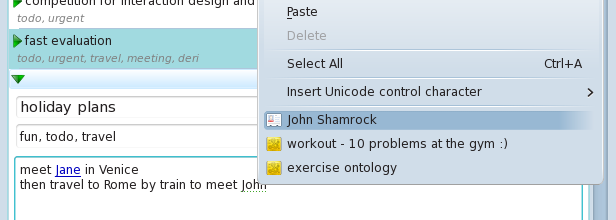
\includegraphics[width=\linewidth]{chapters/core/img/semnotes-screenshot-menu}
\caption{SemNotes annotation suggestion and link.}
\label{fig:annotation}
\end{figure} 

SemNotes does not currently offer suggestions based on online resources\footnote{Similar to \url{www.zemanta.com}.}, unless there is a desktop resource previously created for the relevant Web data (i.e. a bookmarked Web page becomes a desktop resource). 

We are working on an information extractor module, which identifies new information in the content of the notes. It will suggest the creation of new desktop resources from the text, like events, tasks or contacts, that will then be linked to the note. 

Since the annotation suggestions are computed while the user types the note, efficient processing is required. The process of finding possible matches follows:
\begin{enumerate}
 \item Scan the text and identify possible candidates represented by a single word or a sequence of words.
 \item For each possible entity found in the text find a list of existing desktop resources that match it. We use string matching to compute a score for each resource found. The score takes into account the length of the matched string, and if the resource has been linked to the note before.
 \item Sort the matches by score and present them to the user in a non-intrusive way (see Section \ref{sub:semnotesvisualization}).
 \item If the user chooses any of the presented suggestions 
  \begin{itemize}
   \item create a link between the piece of text identified as an entity and the actual resource it represents.
   \item use the selected suggestion in the recalculation of the scores for the entities found for the rest of the note. Once a note is linked to a resource, that resource is more likely to appear again, and therefore it will be ranked higher.
  \end{itemize}
 \item If the user ignores the presented suggestions, no links are created, but the possible matches are saved for later use.  
\end{enumerate}

For the purpose of establishing context, and for organising notes, it is sufficient to create a single link between a note and a resource it is related to, regardless of how many times that resource is mentioned in the content of the note. Therefore the relation between the note and the desktop resource is created only once in the repository. However, if the note is viewed in SemNotes, all the links that the user created to the related resource are displayed.

The interlinking module also manages the removal of links between notes and desktop resources.
Because the suggestion of related resources is based on the content of the notes, once the last textual link to a related resource is removed, so is the relation between the note and the respective resource. 

SemNotes also supports the manual creation of links between the note and desktop resources that are relevant but have no explicit mention in the text.

\subsection{Visualisation}
\label{sub:semnotesvisualization}

SemNotes displays the notes as a list that can be sorted by title, creation or last modification dates, or rating. Each note can be opened in-list for quick access, or maximised over the entire window, for viewing and editing. In the in-list mode, several notes can be open and edited at once (see Figures \ref{fig:screenshot} and \ref{fig:screenshot2notes} for the current version of the SemNotes user interface.).

\begin{figure}[tb]
 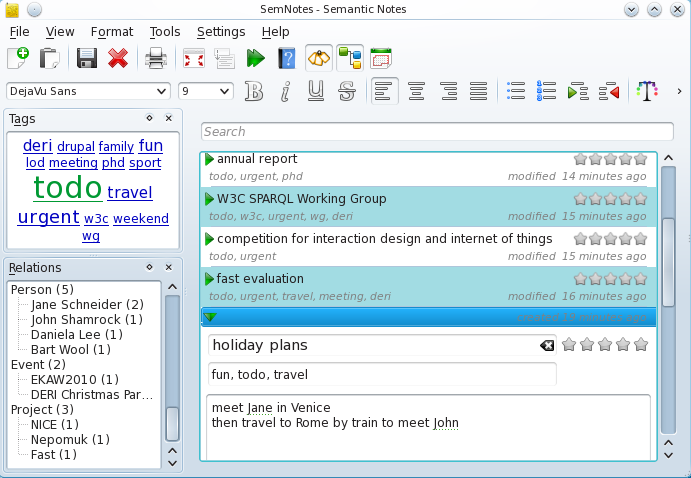
\includegraphics[width=\linewidth]{chapters/core/img/semnotes-screenshot}
\caption{Current version of the SemNotes user interface.}
\label{fig:screenshot}
\end{figure} 

\begin{figure}[tb]
 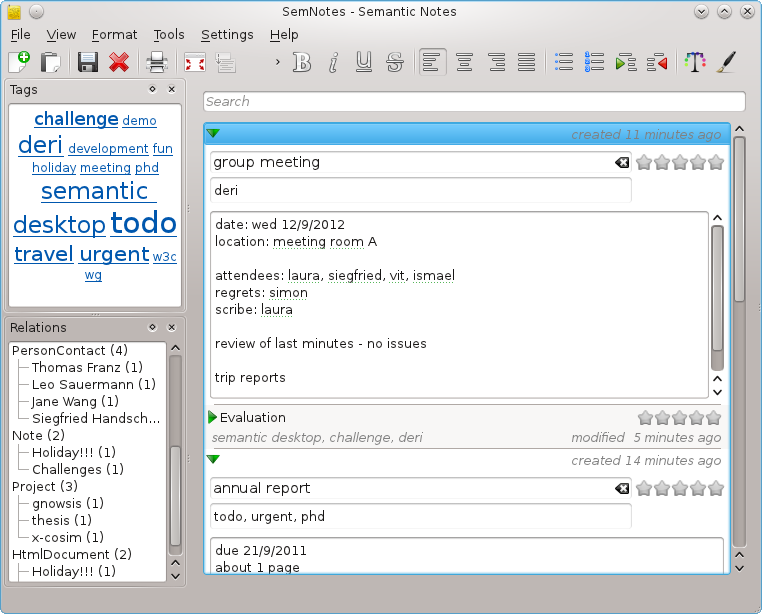
\includegraphics[width=\linewidth]{chapters/core/img/semnotes-screenshot_2notes}
\caption{SemNotes main window, with two notes open in-list.}
\label{fig:screenshot2notes}
\end{figure} 

An aggregated view of the list of notes is based on a restricted set of properties that the notes have in common. Depending on the set of properties used (one or more), the most suitable visual representation of the aggregated view varies. Currently SemNotes offers a tag cloud, a timeline and a related-resource view; each view aggregates information about the notes based on a single property (i.e. the tags associated, the creation date and the related resources, respectively). Aggregated views are displayed adjacent to the list of notes, and can be hidden by the user to allow more space for editing. 

These views also act as a custom faceted browser, as they provide filters on the list of notes. Filtering the list is as easy as clicking on a tag, time interval or related resource. A full text search box also acts as a filter on the list of notes, highlighting the search keywords in the content of open notes, if found. Multiple filters can be set at once, of mixed types. Figure~\ref{fig:screenshot} shows SemNotes with the tag cloud and related-resources views visible, and a tag filter set. A note is open in-list for editing. 

The editor component provides rich text editing of the note content, as well as easy editing of the note metadata. Tagging provides auto-completion based on all the tags on the Semantic Desktop, and creating a new tag is done just by typing its label. If the user does not set a title, SemNotes automatically sets it to the first line of the note. For the rating we used the default visualisation provided by the Nepomuk-KDE libraries, for a uniform interface across the desktop. The creation and last modification dates are the only metadata which cannot be changed through the user interface of SemNotes, as these properties are set automatically. They can be tweaked by expert users, by accessing the RDF repository directly. 

The suggestions for annotations are presented in a simple non-intrusive way, in the ``spell-checker'' style (i.e. the words for which suggestions were found are underlined with a green dotted line instead of a red squiggly line), and are available as context menu items, by right-clicking. Figure~\ref{fig:annotation} depicts how annotation suggestions are presented, and how a linked resource is displayed in the note. To remove an annotation is just as easy as creating it --- through a context menu item.

This presentation of the suggested resources is the result of several iterations of design, each improving on the previous one. 

\begin{figure}[tb]
 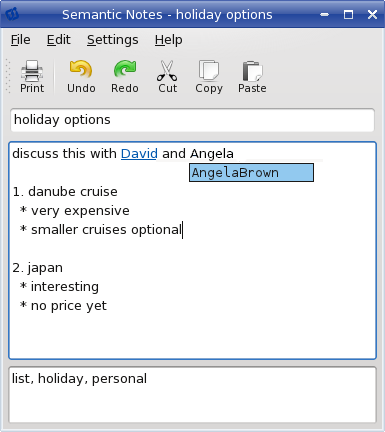
\includegraphics[width=0.6\linewidth]{chapters/core/img/linkednote_v1}
\caption{First version of the SemNotes note editor with pop-up style annotation suggestion.}
\label{fig:popup}
\end{figure} 

The first iteration relied on localised pop-ups with labels of the suggested resources, in the style of text auto-completion (see Figure \ref{fig:popup}). The style worked well when typing the text, and it also enhanced the speed of writing through the auto-completion it provided. The type of annotation of the text during its creation is called latent annotation \cite{Davis2010}, and it is an improvement over the two-step process of first creating the content and then annotating it. Depending on the text of the note, the pop-ups could appear often and distract the user, but they could be dismissed by continuing to type. However, when portions of text were pasted in the editor, several pop-ups were generated at the same time, which was confusing and did not allow the users to make all the connections they would. Changing slightly the pop-ups to only be displayed one-by-one when text was pasted proved not to be a good solution either, as in the case of large paragraphs it would take a long time and many mouse 
clicks for the paste operation to finish, thus interfering with the flow of work. 

Not just the interlinking support was changed from the first version of the application, but the entire user interface. The major redesign was supported by a usability study done as part of the Season of Usability\footnote{\url{http://openusability.org}} 2009, by Daivee Patel, a Human-Computer Interaction student at Drexel University, Philadelphia, USA, with the mentoring help of usability expert Paul Hibbitts of Hibbitts Design, Canada\footnote{\url{http://paulhibbitts.com}}. 
The goals of the project were to recommend changes to improve and/or redesign the SemNotes user interface based on analysis and user research methods, and to perform a usability evaluation of the new changes with a range of users to validate the design recommendations. 

The initial step of the project aimed at forming an understanding of what activities and tasks a user would perform with a note-taking application. This led to the use of a specific technique of task analysis called the activity grid based on the Activity Centred Design methodology. Using this method, we obtained a list of possible activities associated with using a note-taking tool, and each activity was subdivided into the tasks required to perform that activity and each task could then be further subdivided into possible actions. As the tasks became clearer, we identified the tasks that were relevant to SemNotes. These tasks helped focus the effort on the main usability issues and design specifically to address existing issues. 
A comparative analysis of five popular note-taking applications was conducted to help build a knowledge base for reference during the usability inspection of SemNotes. Each of the applications had their own unique features yet certain key functionality appeared standard across these kinds of applications. The examination proved helpful in determining the elements for redesign of the interface. 

The usability inspection of SemNotes was performed to identify usability issues with the existing interface that could be captured without the need to user test before the redesign.
Since the redesign was going to be based on key tasks or activities, we used a heuristic evaluation to identify top level issues.
The criteria for evaluation was the ISO standard ISO 9241\cite{ISO9241}, the principles associated with this standard are based on research and have the benefit of international consensus.
The results of the evaluation were used to help identify areas in the user interface most in need of design improvements, and to create a set of low fidelity mockups. 

A series of usability tests were conducted using the paper prototyping method to validate the initial recommendations for the interface redesign. During each testing session, participants were asked to think aloud and point to elements on the illustrated paper-based screen that they would click or look at based on the tasks provided. No assistance was provided to the users during the testing sessions. The usability test participants were selected via a screening survey on the criteria of experience with computer-based note-taking applications and note-taking habits. 
Based on the feedback from the first set of four users, the mockups were revised for the second round of usability testing while the tasks remained the same. The designs were further enhanced based on the 
feedback received in the second round. 

\begin{table}[htp]
\centering
\ra{1.3}
\begin{tabular}{p{0.45\linewidth} p{0.45\linewidth}}
\toprule
\textbf{Recommendation} & \textbf{Rationale} \\

\midrule
Multi Document Interface (presented as a single window with multiple panes) & By providing all key functionality within a single window, users did not have to manage multiple application windows.\\

Retain optional linking of text within linked editor via use of existing functionality (to click outside the auto complete pop-up) but to be supported by use of icons to indicate the type of resource being linked too & Users showed concern over unwanted text being linked. \\

Search should support searching by tags  & Users realised that since the notes were already tagged during creation, they would like to search by tags for better results. \\

Sorting of notes and tags in the left pane & Multiple options for sorting would help users in locating specific notes and/or tags. \\

First user experience should be provided & Learning curve associated with new applications -- having some introductory information and instructions in the opening screen will be useful. \\

\bottomrule
\end{tabular} 
\caption{Final recommendations for the redesign of SemNotes user interface, based on the usability study.}
\label{tab:sourecommendations}
\end{table}

Based on the accumulated results and feedback, we created a high fidelity mockup of the design, which included all the recommendations (see Table~\ref{tab:sourecommendations}) made as a result of the project, and which were incorporated in the second version of SemNotes.
The next iteration of the display for the annotation suggestions featured a side panel for each of the note edit boxes (see Figure \ref{fig:sidepanel}). The side panel proved to create less interference with the user's workflow, although the suggestions became less obvious. The panel presented the suggestions as a list of resources, that when clicked would highlight the parts of the content to which they were relevant. This helped the users understand from where the suggestion stemmed and if it was indeed correct. To create a link between the note and a suggested resource, the user had to right click on the corresponding item in the list and select ``Link''. Resources could also be removed from the suggestion list, and never be shown again for the current note, to help clear the list from overpopulating. This interface shifted the initial latent annotation style of SemNotes, back to a classic two-step process. Although the suggestions were still computed on the fly, as the user typed or pasted new text, 
because they were out of focus, users were inclined to leave the annotation step for later. Another issue of the side-panel variant was that it limited the screen real-estate for the most important function of SemNotes, that of note-taking. 

\begin{figure}[tb]
 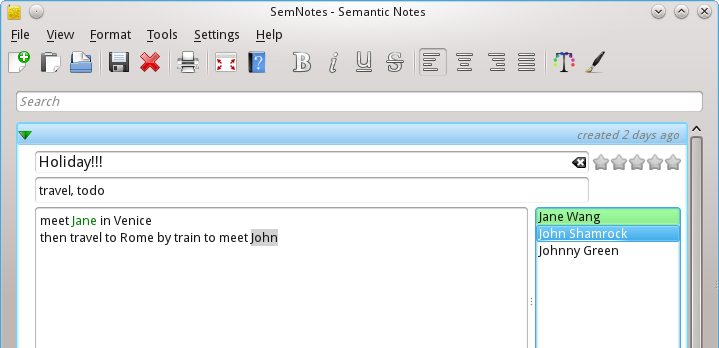
\includegraphics[width=\linewidth]{chapters/core/img/linkednote_v2}
\caption{Second version of the SemNotes note editor with a side panel to display the annotation suggestions.}
\label{fig:sidepanel}
\end{figure} 

To keep more of the screen space for the note editor, in the next iteration, we have abandoned the side panel in favour of the ``spell-checker'' type of notification. It is a mix of the first and second iterations, by giving the users the immediate feedback of the pop-ups, through the green dotted line that underlines words, while being unobtrusive in the note-taking activity. The suggestions are computed on-the-fly like before, but they are only shown if the user right-clicks on the underlined word or words, in keeping with the spell-checker metaphor.

The three iterations of user interface design have improved significantly the usability of SemNotes, as well as the ease of interlinking. However, further usability testing is needed to determine whether and how different types of relations can be created between the notes and the related desktop resources. 


\section{Evaluation}
\label{sec:semnotesevaluation}

We conducted a task-based summative user evaluation, comparing SemNotes to the popular note-taking application Evernote\footnote{\url{http://evernote.com/}}. The goal of the experiment was to determine whether the effort required for the creation of links between notes and resources is repaid by easier search. Towards this goal, we measured the effort needed to execute the same set of tasks with both tools, and compared the results. We used time spent, number of mouse clicks and number of key presses, as measures for effort. After the experiment, we asked the participants about their experience in a questionnaire.

The two applications compared have the same main functionality, note-taking. We chose Evernote as baseline, as it is a very popular note-taking tool that is freely available. Its set of functionalities are richer than those of SemNotes, but the basic features are present and similar in both applications. The feature that distinguishes SemNotes is the same that we want to measure---the creation of links between the notes and desktop resources, based on suggestions given by the application. SemNotes runs on KDE on Linux, and uses the framework provided by Nepomuk-KDE Semantic Desktop. Evernote runs on several operating systems for desktop and mobiles, but Linux is not one of them, therefore we used its Windows version. 

Evaluation is one of the challenges for application design on the Semantic Desktop. Adding to the challenges of evaluating PIM applications with regards to finding appropriate data and tasks for significant measurements, discussed in \cite{Kelly2006}, semantic PIM applications have the difficulty of lacking equivalent semantic tools for a one-on-one comparison. That is why for this evaluation, we followed a methodology similar to the ones described in \cite{Elsweiler2007} and \cite{Franz2009}, of comparing our semantically enabled SemNotes, to a conventional application.

One aspect that we did not evaluate as part of this study is the effect of having the notes connected to the relevant desktop resources from the other applications using the respective resources --- for example, would the extra information from the notes provide an advantage when using a task manager application, and seeing all the linked notes when looking at a task. Such a study would require a longer duration, and also a richer ecosystem of semantic applications, which make use each other's data.

\subsection{Participants} 

Twenty participants took part in the evaluation, all members of our research institute. They are researchers in the field of Semantic Web, thus possibly favouring the semantic application. This bias (if it exists) would however influence only their responses in the questionnaire and not the measured values. Fourteen participants regularly use note-taking and five of them use Evernote as their preferred note-taking tool. None of the participants used Linux as their operating system. Their familiarity with one environment and one application could have influenced the measured results, in favour of Evernote.

\begin{figure}[htb]
 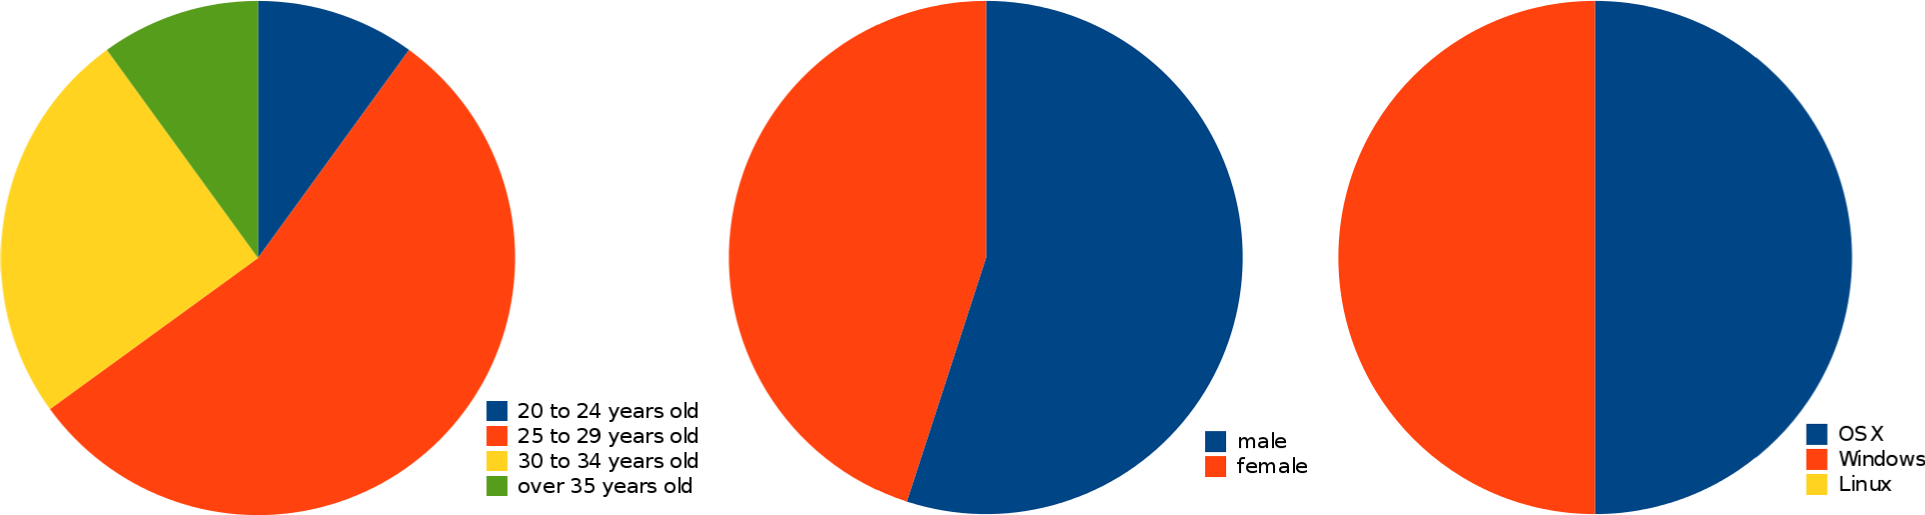
\includegraphics[width=0.95\linewidth]{chapters/core/img/distribs}
\caption{Age, gender and OS distributions of participants.}
\label{fig:distribs}
\end{figure}

Some additional demographic details of the participants: gender distribution was close to even (eleven men and nine women); most of them were in the age groups between 25 and 29 (eleven, equivalent to 55\%), and between 30 and 34 (five, or 25\%). There were seven Master's students, seven Ph.D. students, five senior researchers and one intern. For demographic distributions see Figure \ref{fig:distribs} and Figure \ref{fig:genderdistribs}.

\begin{figure}[htb]
 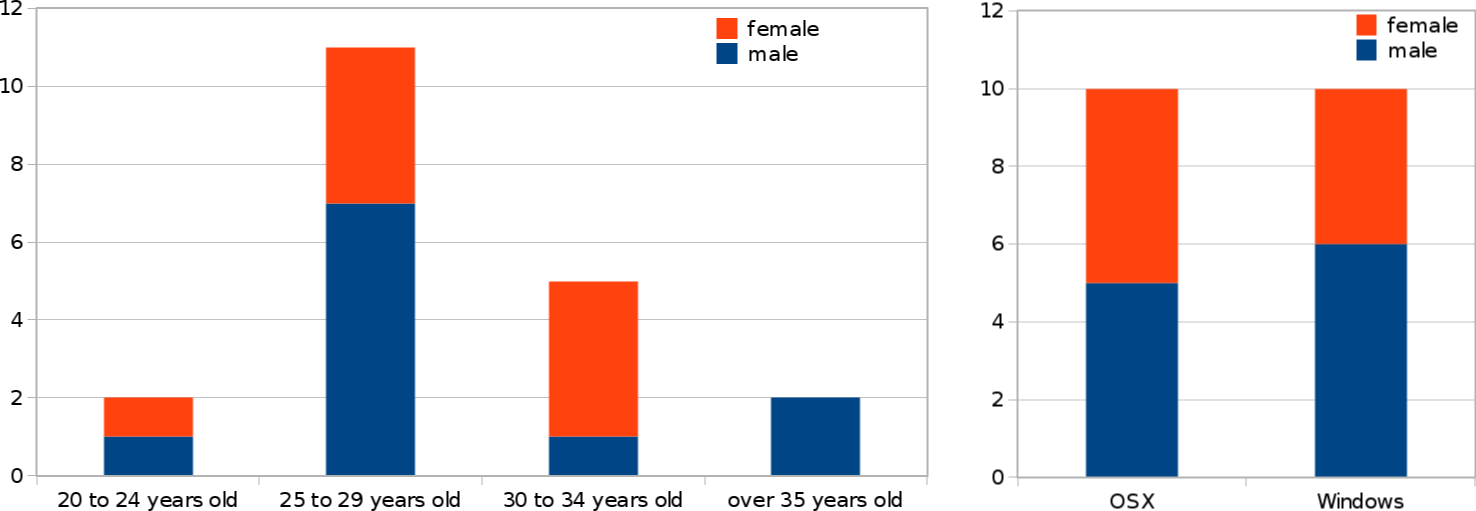
\includegraphics[width=0.9\linewidth]{chapters/core/img/genderdistribs}
\caption{Age and OS distributions of participants per gender.}
\label{fig:genderdistribs}
\end{figure}

\subsection{Data} 

We used two virtual machines for the experiment, preloaded with identical data. To reduce the artificialness of the study, we chose general data familiar to the participants, to which they have access in their everyday work. The dataset contained contact information for 130 members of our institute; 655 recent emails from our mailing lists; 20 scientific papers authored by our colleagues; and photographs from institute events. The note data was also identical: 50 notes on a variety of topics, personal or work-related, tagged with 23 tags. In SemNotes, we also provided links between the notes and the resources mentioned in them: people, projects, events or other notes, within reasonable limits we expect users to interlink their notes (i.e. minimum 0 links, maximum 10 links, average 1.8, median 1). The majority of connections were made to people mentioned in the notes.

\subsection{Tasks} 

We prepared a set of eight tasks. Each participant was requested to run all the tasks in each of the two environments. To prevent order effects from influencing the results, half of the participants started with SemNotes and the other half with Evernote.

\begin{description}
 \item[T1.] Find what information is available about yourself (contact information, documents, emails, photographs)
 \item[T2.] Find the paper titled ``Bridging the Gap between Linked Data and the Semantic Web''. Who are the authors?
 \item[T3.] Find notes tagged with ``todo''.
 \item[T4.] Find to-dos that are related to our institute.
 \item[T5.] Find a to-do related to a presentation by a colleague John.
 \item[T6.] Take a note about planning a social event for your research group. Write the names of two people that have already confirmed. Annotate the note as you see fit.
 \item[T7.] Find a note containing the minutes from the last meeting about a given project. Change the date of the next meeting planned.
 \item[T8.] Take a new note for the action item assigned to you at the last meeting of the project. The action item is in the meeting minutes previously edited, and it requires drafting a document using a paper authored by a colleague. Annotate the note.
\end{description}

The first two tasks were intended to help the participants get accustomed with the data available and the environment; we did not include the time spent on these tasks in the results. 

The last six tasks were focused on note-taking, and their complexity increased gradually. T3, T4, and T5 are search and filter tasks (S), from the very simple to the complex. T6 and T8 are editing tasks (E), including any annotations that the participants made on the notes. T7 is both a search and edit task (SE). It prepares the participants for the most complex search and edit task, T8, which required interaction with the rest of the system (i.e. finding the required paper).

\subsection{Measurements} 

The participants were recorded while doing the tasks of the experiment, and the videos were used to extract the measurements used in the analysis. 
For each task we measured the effort in seconds spent, and number of mouse clicks. 
We also counted the number of key strokes for the tasks involving creation of notes, and we used this measure to normalise the values for time. 
Although we had two separate measures for each task, we were interested in the difference between these values, computed according to:
$$
value_{difference} = value_{SemNotes} - value_{Evernote}
$$
Thus, a positive value means that the value recorded for SemNotes is bigger than the corresponding value for Evernote, and a negative value means that the value for SemNotes is smaller. 

For the time measurements, the time difference represents the extra \emph{effort} required for annotating the notes with links in the editing tasks. For the search tasks the difference shows which of the applications enables the users to find the notes easier, thus the \emph{benefit}. We must specify here that actual searches done by the software were considered instantaneous, as the datasets are small and we did not intend to measure the performance of the search algorithms used.

For the number of mouse clicks, the difference represents the extra \emph{effort} required, for both types of tasks.

\begin{figure}[tb]
\begin{center}$
 \begin{array}{ccc}
  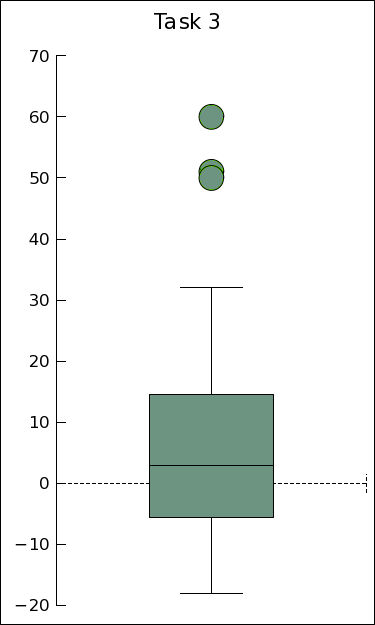
\includegraphics[width=0.29\linewidth]{chapters/core/img/task3difboxplot} &
  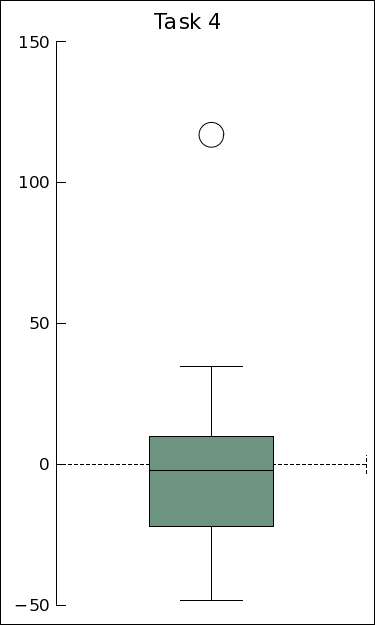
\includegraphics[width=0.29\linewidth]{chapters/core/img/task4difboxplot} &
  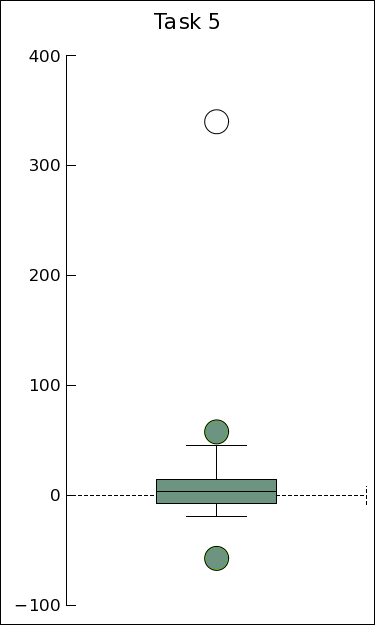
\includegraphics[width=0.29\linewidth]{chapters/core/img/task5difboxplot} \\ 
  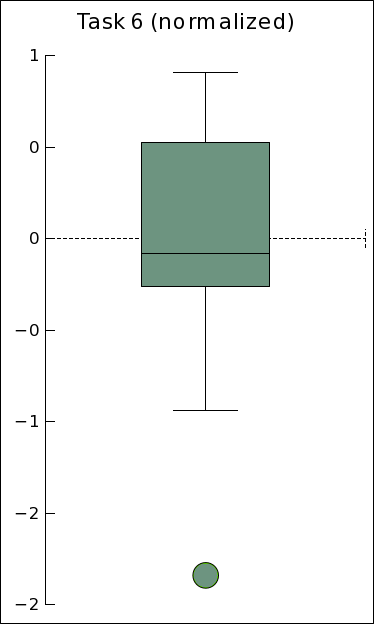
\includegraphics[width=0.29\linewidth]{chapters/core/img/task6difboxplot} &
  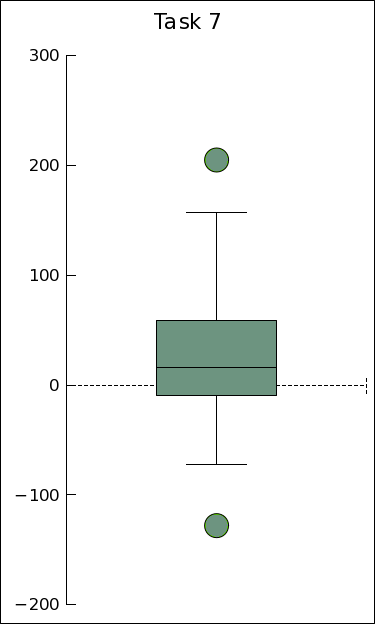
\includegraphics[width=0.29\linewidth]{chapters/core/img/task7difboxplot} &
  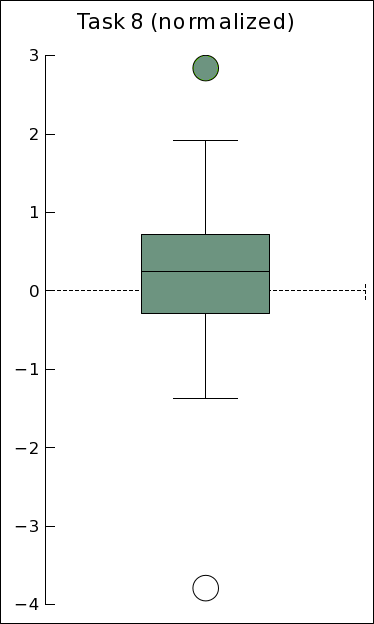
\includegraphics[width=0.29\linewidth]{chapters/core/img/task8difboxplot} 
 \end{array}$
\end{center}
\caption{Inter-quartile ranges for the time difference.}
\label{fig:boxplots}
\end{figure}

After a first analysis of the results, we noticed that some values for time were unrealistically high or low. They coincided with the measurements when the participants stopped to ask a question or comment on a feature. We decided to eliminate these outlier values by using only the measurements that fall in the inter-quartile range, for all tasks --- see Figure \ref{fig:boxplots}.

\subsection{Quantitative Results}

We tested if the effort measured in time and mouse clicks was different when using SemNotes than when using Evernote. Table \ref{tab:semnotesresults} shows the results, with the statistically significant values in bold (\begin{math}p < 0.05 \end{math}).

\begin{table}[htp]
\centering
\ra{1.3}
\begin{tabular}{@{}clcr@{.}lr@{.}lr@{.}lcr@{.}lr@{.}lr@{.}l}
\toprule
\multirow{2}{*}{\textbf{T}} &&& \multicolumn{6}{c}{\textbf{Time (s)}} && \multicolumn{6}{c}{\textbf{Clicks}} \\

&&& \multicolumn{2}{c}{\textbf{Avg}} & \multicolumn{2}{c}{\textbf{Med}} & \multicolumn{2}{c}{\textbf{\textit{t}}} && \multicolumn{2}{c}{\textbf{Avg}} & \multicolumn{2}{c}{\textbf{Med}} & \multicolumn{2}{c}{\textbf{\textit{t}}} \\
\midrule
\textbf{T3} & (S) && 0 & 5 & 0 & 0 & 0 & 152 && 0 & 167 & 0 & 0 & 0 & 692 \\

\textbf{T4} & (S) && -8 & 0 & -8 & 0 & \textbf{-2} & \textbf{94} && -0 & 333 & -1 & 0 & -0 & 48 \\

\textbf{T5} & (S) && -0 & 125 & 1 & 0 & -0 & 046 && 0 & 857 & 1 & 0 & 1 & 426 \\

\textbf{T6} & (E) && 0 & 063 & 0 & 016 & 0 & 486 && 6 & 067 & 8 & 0 & 2 & 026 \\

\textbf{T7} & (SE) && 14 & 357 & 13 & 0 & 1 & 713 && 4 & 812 & 2 & 0 & 1 & 527 \\

\textbf{T8} & (SE) && 0 & 249 & 0 & 243 & 1 & 004 && 20 & 8 & 12 & 0 & \textbf{3} & \textbf{08} \\

\bottomrule
\end{tabular} 
\caption{Statistics for time and click differences.}
\label{tab:semnotesresults}
\end{table}

Results show that for the simple search task T3 the difference is positive, which suggests that it takes longer to finish the task with SemNotes. However, the difference is not significant. For the complex search tasks that follow, T4 and T5 the difference has negative values, showing that the users spent less time on complex searches when using SemNotes, thus supporting the claim that the use of interlinked data makes notes easier to find. Only the results for T4 are statistically significant. None of the measures of number of mouse clicks for the search tasks are statistically significant, the differences being in average less than 1 click, with a median value of 0, -1 and +1 respectively for the tasks T3, T4 and T5.

For the editing task T6, the values are positive, thus it took longer to finish it with SemNotes. This was expected, as in SemNotes there is the additional step of annotating the notes with links to desktop resources. However, the differences are very close to 0 (0.063s average and 0.016s median) and not statistically significant. This editing task did require in average 6 more mouse clicks in SemNotes, with a median value of 8, but the difference is also not statistically significant.

For the more complex search and edit tasks T7 and T8, the time differences, while positive, thus in favour of Evernote, are not significant. For both tasks the values were positive, which mean more clicks when using SemNotes. However, task T8, that required creating and annotating a complex note based on information from other sources, had statistical significant difference in number of clicks, in favour of Evernote (more clicks needed in SemNotes). 

The positive difference in the number of clicks required for all editing tasks (T6, T7 and T8) is not surprising, as the participants recognised the value of creating links and proceeded to link the new note to the relevant resources. This was however a motivation for providing better keyboard support for the annotation of notes in the future version of the tool.

In summary, the results show that there are significant improvements (for one of two tasks) in the time spent on complex searches, when the data is interlinked, at no significant extra cost for the creation of the links. Linking does however significantly increase the effort measured by number of mouse clicks (for one of two tasks).

\subsection{Questionnaire}

We asked the participants to fill in an anonymous questionnaire related to the experiment. The questionnaire is listed in Appendix~\ref{ap:questionnaire}. According to the answers, on a scale from 1 to 5, the tasks were simple (mean 2.25) and similar to the ones in their daily work (mean 3.4), and the data provided was familiar (mean 3.2). 

The answers also show that 60\% of the participants (12) felt that SemNotes helped them finish the tasks \emph{faster}, while only 20\% (4) said Evernote, and 20\% did not feel any difference between the tools. When asked which of the two applications helped them perform the tasks \emph{better}, 80\% of the participants chose SemNotes, while the remaining 20\% did not feel that there was any difference (see Figure \ref{fig:betterfaster} for a graphical representation).

\begin{figure}[htb]
 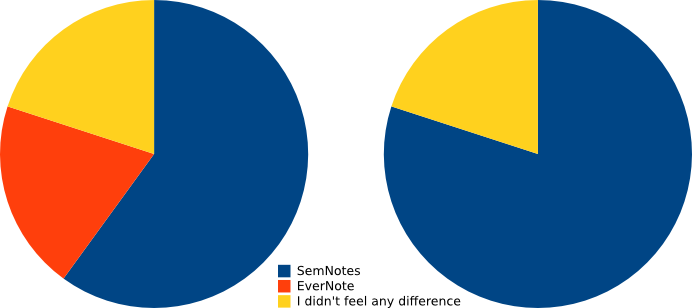
\includegraphics[width=0.7\linewidth]{chapters/core/img/fasterbetter}
\caption{Which tool helped perform the tasks faster (left) and better (right).}
\label{fig:betterfaster}
\end{figure}

The participants had a good overall impression of SemNotes (with a mean of 4.15 on a scale from 1 to 5). This rating was supported by comments like ``\emph{That was cool.}'', and requests for SemNotes for other operating systems: ``\emph{Maybe you could make an OS X version?}'' and ``\emph{When is a port for Windows 7 coming?}''.

The semantic annotation was one of the most liked features of SemNotes, and one of the features most missed in Evernote, according to the questionnaire. Another advantage of SemNotes was considered the multiple filtering by mixed criteria, with several participants considering it the best feature. The rating of notes was listed as the least liked feature of SemNotes by three participants. The tag cloud was the most controversial feature, as many participants liked it and found it very useful, while others would have preferred a simple list of tags: ``\emph{Usually I don't like tag clouds, but the one in SemNotes was really useful.}'' and ``\emph{While the tag cloud helps in determining the most used tag, a simple list with the tags seems to be easier to search.}'' 


\section{Related Work}
\label{sec:notetakingapps}

Semantic note-taking means enhancing the note-taking process using Semantic Web technologies. It can refer to the techniques and methods used in the implementation, like ontologies and RDF, but most importantly it is about creating a semantic network around the notes and the information contained in them. There are several applications that enable more or less semantic note-taking: some are browser based (online or offline), while others are standalone desktop applications as is SemNotes. 

The List.it browser-based note-taking tool \cite{Kleek2009} and Jourknow, its predecessor \cite{Kleek2007}, save context alongside the information scraps, to improve re-finding and reminding. List.it also features information extraction from the unstructured text of the notes, recognising entities and relations between them, with the \emph{pidgin} language processor. However, unlike SemNotes, the contex of the notes they create does not include links to any existing desktop resources. SnapShoot \cite{Iga2006} is another browser-based note-taking tool that explores new visualisation techniques to improve reading of the documents produced. It features categorisation, and limited interlinking with documents within the system.

MindRaider \cite{MindRaider}, described above in Section \ref{sec:sdsystems}, is an open source ``Semantic Web outliner'' and extended note-taking system for information organisation. While it only interlinks concepts within its maps, it can connect to the Gnowsis Semantic Desktop through a plugin, thus potentially it can use any Semantic Desktop resources through a similar mechanism.

A distinct category of semantic note-taking applications are personal semantic wikis, like Kaukolu \cite{Elst2008}, IkeWiki \cite{Schaffert2006} and GDKTiddlyWiki. Each wiki page represents a resource and its semantic relations to other resources are encoded within the page, using an extension to the wiki syntax. Only predefined relations and types are available, and the wikis offer limited access to other desktop information sources. Unlike SemNotes, connections are only possible between resources within the wiki system.

OneNote from Microsoft's office suite provides quasi-se\-man\-tic functionality by interlinking the notes with address book information, calendar, and tasks. It does not use any semantic technologies though, and the data is locked in by proprietary formats and storage.

Zemanta\footnote{\url{http://www.zemanta.com}} is a blog assistant that suggests possible enhancements to blog posts, like linking external content and images. Unlike SemNotes, which uses the local repository to search for matches, Zemanta looks on the Web. It does not assign any semantics to the links. 

There are also specialised systems like the SemanticPen \cite{Varadarajan2005} which provides support for semantic note-taking with pen devices.
Other note-taking applications that provide semantic features include: Jenga Note\footnote{\url{http://www.jenganote.org}} --- allows associating a note with a concept, Catch Notes\footnote{\url{http://www.catch.com}}, and SpringPad\footnote{\url{http://www.springpadit.com}}.


\section{Conclusion}

In this chapter, we presented a solution to the challenges of designing applications for the Semantic Desktop. We described one such application, SemNotes, a semantic note-taking tool for the Nepomuk-KDE Semantic Desktop. It provides a real-world, functional use case for fully exploiting the capabilities of the Semantic Desktop: interlinking, organisation and management of personal information, efficient search and browsing. It supports the entire life-cycle of the semantic data represented by notes, with emphasis on the creation of links between the new data and the existing network of linked information on the desktop. 

Through SemNotes we present a possible solution to each of the challenges presented in the begining of the chapter. To the first question of creating semantic data, we describe how we create new semantic notes, using the existing vocabularies and creating links to the existing Semantic Desktop data available. To the second question of designing the human computer interaction, we describe the efforts towards an easy to use yet rich user interface design for SemNotes. With the help of usability experts and user testing the interface went so far through three iterations, each described in this chapter.

For the third challenge, that of evaluating a semantic tool, we described a task-based user evaluation comparing SemNotes to the popular note-taking application Evernote. The results show that the extra effort (measured in time spent) required for the annotation of notes with links to related resources is not significant. However, the benefit (measured in time saved) is significant for one of two complex search tasks. 

SemNotes embodies a simple and user-friendly way of generating new semantic data on the desktop, and integrating it with the already existing data. However, the personal information that the users work with is not restricted to the desktop. Further, semantic data exists in large quantities outside of the desktop, on the Web and in organisational repositories. Thus, in the next chapter we continue by describing how the linked information from the desktop can be meaningfully and safely connected to the outside world.


\chapter{Bridging the Gap between the Semantic Desktop and the Web of Data}
\label{ch:sdwod}

\begin{flushright}
 \textit{Based on ``Linking Semantic Desktop Data to the Web of Data'' \cite{Dragan2011b}\\published at the 10th International Semantic Web Conference (ISWC~2011)}
\end{flushright}

The previous chapters showed how the Semantic Desktop enables better personal information management on our computers, using semantic technologies to explicitly connect information which is naturally connected in the real-world, and thus matching the representation to a user's mental model. However, our personal data is often a reflection of our subjective view, or limited knowledge. Thus, although it may seem huge when faced with the task of organising it, the information on the desktop is small compared to the amount of information available online. The Web of Data contains a linked network of information similar to the one on the desktop, only at a much larger scale. Connecting the desktop to the Web of Data would enrich and complement desktop information.

This chapter presents a solution to the second research question \textbf{Q 2.} from Section \ref{sub:question}, \emph{how to expand the scope of the Semantic Desktop into the realm of the Web of Data, to enhance the user experience and benefit?}, more specifically, to the first sub-question \textbf{Q 2.1.} described there --- \emph{how to find instances representing the same real-world thing described by a Semantic Desktop resource?}

Our solution uses a semantic search engine for the Web of Data, such as Sindice\footnote{\url{http://sindice.com/}}, to find and retrieve a relevant subset of entities from the Web. We present a matching framework, using a combination of configurable heuristics and rules to compare data graphs, that achieves a high degree of precision for the linking decision.
We evaluate our methodology with real-world data --- we create a gold standard from relevance judgements by experts; and measure the performance of our system against it. We thus show that it is possible to automatically link desktop data with Web data in an effective way.

\section{Introduction}
\label{sec:sdwodintro}

The Semantic Desktop aims to enable better organisation of the personal information on our computers, by applying semantic technologies on the desktop. Just as Linked Data connects distributed data on the Web, creating a network of interlinked information, the Semantic Desktop connects personal data across application boundaries on the desktop, creating a network of personal information.
However, information on our desktop is often incomplete, as it is based on our subjective view, or limited knowledge about an entity.

On the other hand, the Web of Data contains information about virtually everything, generated by multiple sources, and theoretically unlimited. Connecting the desktop to the Web of Data would thus enrich and complement desktop information. Bringing in information automatically from the Web of Data would release the user from the burden of searching for information.

Connecting the two networks of information opens up the possibility of personal services on the desktop, which use external data but in the personal context of the user, highly connected to his personal data and focused on his interests. One such example is a service that finds implicit links between the publications that the user has on the desktop, and provides recommendations to other publications on the same topics, by the same authors, or related in another way. 
Another desktop service could use information from the Web of Data to notify the user of new concert dates in his area, based on the latest or most popular artists played on the desktop. 
Web data can also be used as a point of reference when working collaboratively, e.g., documents linked by the user to people, projects, or other resources from his semantic desktop can be shared together with the annotations, which can be accessed and reused outside of the Semantic Desktop where they were generated.

From the perspective of interlinking information, and using the frameworks provided by the Semantic Desktop and the Web of Data, we have separate islands of knowledge, both containing similar data, related to the same topics of interest to the user, but disconnected from each other. 

The disconnection appears in two forms:
\begin{itemize}
 \item The data on the desktop, although similar to that on the Web of Data, is described using specific \emph{desktop ontologies}, which are different from the ones found on the Web of Data. This schema mismatch makes interlinking data from the two datasets difficult.
 \item Identifiers (URIs) on the desktop are local to the desktop data space, they are not globally unique and cannot be dereferenced as normal Linked Data URIs are. Hence, it is hard to access and connect to local data from the Web.
\end{itemize}

To tackle this disconnection, it is necessary to create links between desktop identifiers and Web identifiers that refer to the same real-world thing.
This means we need to compare the data graph describing an entity on the desktop with the data graph of an entity on the Web. Leaving aside the use of different terminology within the data, the Web of Data is large, with billions of entities across hundreds of thousands of datasets. From this vast amount of information we must find and retrieve a relevant subset of entities, that are potential candidates with the desktop entity. Then we must decide if the candidates are similar enough with the desktop entity to create a link between the two. Because we wish to make the interlinking automatic, we must be able to decide with a high degree of precision which candidates among this subset are in fact referring to the same entity.

Our solution tackles the problems raised above by using a semantic search engine for the Web of Data, such as Sindice, to find and retrieve
a relevant subset of entities from the Web. We then present a matching framework, using a combination of configurable heuristics and rules to
compare data graphs, that achieves a high degree of precision in the linking decision. 

To evaluate our methodology with real-world data, we create a gold standard from relevance judgements by experts, and we measure the performance of our system against it.

Our solution proves that interlinking the two environments is feasible, and even more, it yields good results. Connecting desktop data with the Web enables the system to bring Web data to the users, instead of the users having to go find it by themselves.


\section{Related Work}
\label{sub:sdwodrelatedwork}

The problem of entity linking is well known across various research communities with a variety of different names, such as record linkage \cite{Felligi1969}, entity resolution \cite{Benjelloun2006}, reference reconciliation \cite{Dong2005b} or object consolidation \cite{Hogan2007}. A wide variety of algorithms has been developed for resolving the co-reference problem, but record linkage between distributed databases is still considered a  difficult problem.

Recent initiatives within the Semantic Web community address the problem of linking entities across data sources. For instance, \cite{Jaffri2007} describe the phenomenon of proliferation of URIs and propose a Consistent Reference Service to manage URI equivalences. The OKKAM project \cite{Bouquet2007} proposes an infrastructure for assigning global identifiers at web scale. These approaches are more focussed towards the management of entity identity on the Web, but do not provide an easy means to create new links between data sources. 

Similar to our approach, \cite{Raimond2008} describe an algorithm and its implementation GNAT, for linking a personal music collection to corresponding MusicBrainz resources. The approach recursively measures the similarity of the resource graphs from the two datasets, with the limitation that the same vocabularies must be used in both. By contrast, using property paths in our mappings, we eliminate the need for recursion while still propagating the measures from connected resources.
Silk is a framework for linking multiple entities between two datasets \cite{Bizer2009}. It relies on user-defined rules and various string matching algorithms to measure the similarity between two entities. In this case it is necessary to know a priori which specific dataset to link to and to perform manual configuration of the matching algorithms, something that requires a high degree of expertise.
\cite{Hogan2007} and \cite{Sais2007} propose logic-based methodologies for merging identifiers of equivalent entities across multiples knowledge sources. While being precise, these techniques do not have a very good recall and are computationally demanding.

The most relevant approach related to ours is the Silk framework. We provide a generic matching process that the user can configure based on their own expertise in order to get more precise results. However, our approach differs by the fact that the matching process is not restricted to linking data between two predefined information sources. On the contrary, our approach makes it possible to link desktop data with an arbitrary number of external data sources. This makes the problem harder since we are generally unaware of the data structure or schema of these data sources. 

We therefore need to first find potential entities of interest among a vast number of data sources, then retrieve a partial description of these entities and rely on more complex entity matching algorithms. 

This first step of our algorithm can be seen as a blocking pass to reduce the information space before executing complex matching algorithms \cite{Elmagarmid2007}. The blocking step is implemented on top of a boolean query model for centralised search systems such as Sindice \cite{Tummarello2007} and on top of the SPARQL query language for specific data sources providing a SPARQL endpoint.

\cite{Nikolov2012} propose the use of a genetic algorithm to achieve unsupervised discovery of the similarity parameters needed for data linking between two datasets. Similarly to our algorithm, the approach proposed uses a blocking pass using a SPARQL query, to reduce the computation time. As with Silk, the algorithm considers only two datasets to be matched.


\section{The Process of Finding Web Aliases}
\label{sec:process}

The goal of our algorithm and system is to find Web aliases for desktop resources. A Web alias is a Web entity identifier, i.e., URI, that represents the same real-world thing as the desktop entity to which it was matched. To find Web aliases, we use the information available on the desktop, like the contact information from the address book for people, or metadata of music files for songs, albums and artists. We also use the knowledge about the desktop ontologies and the way data is organised and used on the desktop. The desktop data drives the entire process, and is used throughout the steps:

\begin{enumerate}
 \item Candidate selection --- blocking pass
 \begin{itemize}
  \item Query and identify candidate entities from various Web of Data sources
  \item Retrieve data for each candidate from the appropriate source[s].
 \end{itemize}
 \item Candidate filtering --- scoring based on similarity
 \begin{itemize}
  \item Compute similarity score based on the data of the entities.
  \item Filter the candidates based on the similarity score.
 \end{itemize}
\end{enumerate}

The first step requires identifying a list of candidate entities and obtaining the data available about them. There are two options for this:

\begin{itemize} 
\item through a small set of sources that we know have the data we need, and can query each of them independently for possible candidates, or 
\item through a search engine for the Web of Data, like Sindice \cite{Tummarello2007} which indexes millions of documents containing semantic mark-up.
\end{itemize}
Each option has use cases where it is more suitable than the other, thus we designed our system to support both. Querying specific sources is preferred for instance, if the data is from a very specific domain, like cancer research, or when we are interested only in results from an organisation's internal repository. Using a search engine is best when the information sources to query are not known a priori. It also has the advantage of covering a large number of information sources with only one query, and of selecting the most relevant data sources and candidates with respect to the query via the search engine ranking system. However, in the case of ambiguous entities, the latter option has the disadvantage of returning too many unrelated results, thus making the entity selection more difficult.

Once a list of candidates is available, we compute a similarity score for each of them with respect to the desktop entity. The desktop data is considered authoritative, and the matching process is driven by it. This has the apparent advantage of control, since the desktop data is more strictly under the control of the user. However, there are cases when the desktop data is simply insufficient, or has uncaught errors due to the user's incomplete information, or the Semantic Desktop's extraction process.

The matching algorithm checks first whether the types of the candidate entities correspond to the type of the desktop entity, and discards the ones that do not.
Only then are the data of the entities examined and the properties and corresponding values compared. If required, the algorithm looks at other related entities and their properties. The values of the properties are compared using either exact string matching or string similarity techniques. As mentioned above, the ontologies used on the desktop are different from those used on the Web, thus both type checking and property matching require mappings between the two sets of vocabularies.

After the matching algorithm computes the scores for each of the candidates, the list is filtered for values above a given threshold. References to those Web resources which passed are saved in the desktop repository, as \verb|pimo:hasOtherRepresentation| links from the initial desktop resource.


\section{Implementing the Process}

We implemented the process described above in a desktop daemon that finds Web aliases for desktop entities.
It sequentially searches for aliases for all resources that have no alias listed, and for resources that have changed since the last time aliases were determined for them. In the case when a resource is revisited after being modified, the previously found aliases are discarded and new ones are searched for.

The result of the process is the creation of new links on the Semantic Desktop between local resources and their Web aliases. They can be used to enhance the desktop data about the entities, or as entry points to access further information online.

The implementation has two major components, each handling one step of the matching process: A query component that initiates the search and identifies the candidates, and a matching component that filters the candidates based on similarity measures. We next discuss these components in turn.

\subsection{The Query Component}
\label{sub:querymodule}

The query component was designed to be able to use either generic search engines or specific data sources. Therefore, we chose to make the query module plugin-based, thus allowing various new sources to be connected if needed. The query modules are responsible for finding the initial list of candidates, as well as for retrieving the data for each candidate. The maximum number of candidates to retrieve from a data source can be set as a parameter in the configuration. We allow three types of plugins:
\begin{description}
 \item[SWSE] --- connect to semantic search engines, through their APIs. We provide a plugin of this type for Sindice.
 \item[Sparql] --- connect to sources that provide a SPARQL endpoint. We provide plugins of this type for DBpedia and the Semantic Web Conference Server.
 \item[Custom] --- connect to other sources, possibly ones that do not expose any data as RDF (e.g., relational databases or third-party APIs like last.fm).
 \end{description}

Most major Linked Data providers (e.g. DBpedia) are indexed by Sindice, therefore the Sindice plugin is the only one enabled by default.

In the Sindice module, the initial query, which determines the list of candidates, is constructed using all the value properties of the desktop entity, combined using the boolean conjunction operator ``OR''. Multiple word terms are also tokenised and the tokens are added to the query. This may result into a longer query which contains duplicate words. This is however due to the fact that we rely on the search engine to interpret the query and rank higher the results that match most of the terms. The search engine (in this case Sindice) algorithm ranks higher results which match more of the strings connected by ``OR''. Building the query with just the strings without quotes would result in automatic tokenisation by the search engine, which might lead to higher ranking of unsuitable results, especially if the words searched for are common. Thus we chose to prevent the tokenisation by the search engine by using quotes around the full string searched for, but still mimic the default behaviour of the algorithm by 
doing the tokenisation ourselves, as a fail-safe in case the query yields no results. 

For the music album ``One Night Only'' by the Bee Gees from 1998,  the query constructed is:

\begin{quote}
 \emph{``Bee Gees'' OR ``One Night Only'' OR ``1998'' OR ``Bee'' OR ``Gees'' OR ``One'' OR ``Night'' OR ``Only''}
\end{quote}

\subsection{The Matching Component}
\label{sub:matchingcomp}

The matching module computes a similarity score for each pair $($\emph{desktop~entity}---\emph{web~candidate~entity}$)$. The way the score is computed depends on a set of parameters:

\begin{description}
 \item[String matching (SM)] --- If this parameter is set to \texttt{true}, the matching module will use string similarity measures where appropriate. Currently the system supports Monge-Elkan \cite{Monge1996} and Chapman\footnote{\url{http://sourceforge.net/projects/simmetrics/}} distances. If the value is set to \texttt{false}, the matching module uses exact matching of property values.
 \item[Weighted properties (WP)] --- If \texttt{true}, the matching module will use weights for the properties compared, otherwise, all properties contribute equally to the final score.
 \item[Multi-valued properties (MVP)] --- If \texttt{true}, properties that have more than one matching value will contribute to the score proportionally to the number of values. 
 \end{description}

These parameters are set by default to true. However, the measurements we did for the evaluation (see Section \ref{sec:sdwodeval}) show that in some cases they can be disabled without impacting the quality of the result, while requiring less processing; or even make the algorithm perform slightly better when disabled, for some restrictions.

\lstset{
	caption={Type mapping for pimo:Person.}, 
	label=lst:typemapping,
	language=js
}
\setlength\parindent{0in}
\begin{minipage}[htb]{\linewidth}
\begin{lstlisting}
{
   "http://www.semanticdesktop.org/ontologies/2007/11/01/pimo#Person": {
      "mapping":[
         "http://xmlns.com/foaf/0.1/Person",
         "http://xmlns.com/foaf/0.1/Agent",
         "http://dbpedia.org/ontology/Person",
         "http://www.w3.org/2000/10/swap/pim/contact#Person",
         "http://rdf.data-vocabulary.org#Person" 
      ]
   }
}
\end{lstlisting}
\end{minipage}
\setlength\parindent{0.21in}

\lstset{
	caption={Property mapping for nco:fullname of nmm:performer.}, 
	label=lst:propmapping,
	language=js
}
\setlength\parindent{0in}
\begin{minipage}[htb]{\linewidth}
\begin{lstlisting}
{
   "http://www.semantcdesktop.org/ontologies/2009/02/19/nmm#performer##http://www.semanticdesktop.org/ontologies/2007/03/22/nco#fullname": {
      "mapping": [
         "http://dbpedia.org/property/artist",
         "http://dbpedia.org/ontology/artist##http://xmlns.com/foaf/0.1/name",
         "http://xmlns.com/foaf/0.1/maker##http://xmlns.com/foaf/0.1/name"
      ],
      "approx":"true",
      "thresholds": [
         "MongeElkan:0.7",
         "Chapman:0.8"
      ],
      "weight":"0.7" 
   }
}
\end{lstlisting}
\end{minipage}
\setlength\parindent{0.21in}

The algorithm uses a set of mappings from the desktop ontologies to some of the more popular Web vocabularies, like FOAF. There are two kinds: \emph{type mappings} (see Listing~\ref{lst:typemapping} for an example) and \emph{property mappings}, each described in a separate file. The property mapping supports paths of properties. For example,  Listing~\ref{lst:propmapping} shows a path composed of the property \texttt{dbpedia:artist} and \texttt{foaf:name}. The mappings are relatively static configurations of the system. We have created a set of mappings for the most common ontologies, which can be used out of the box by the end users. Power users can edit the mapping files according to their needs. We envision that as more users find the system useful, more mappings will be created and shared.

\subsubsection{The scoring and matching algorithm}

The algorithm for computing the score works as follows. Given a pair of entities to be compared $e_{d}$ and $e_{w}$, it first determines the sets of types $T_{e_{d}}$ and $T_{e_{w}}$ for each entity, and the set of types $Map[T_{e_{d}}]$ to which the elements of $T_{e_{d}}$ are mapped. If no types are matching, i.e., $T_{e_{w}} \cap Map[T_{e_{d}}] = \phi$, it gives a score $score(e_{w}) = 0$, and stops the matching. Otherwise, it continues the process by evaluating the properties.

The evaluation of the properties is driven by the relations and properties of the desktop entity $e_{d}$. For each property $p_{e_{d}}$, the algorithm retrieves the list of values $V(p_{e_{d}}) = \{v\ :\ \{e_{d}\ p_{e_{d}}\ v\}\}$. Based on the list of property mappings $Map[p_{e_{d}}]$, it determines the set of values $V(p_{e_{w}} \cap Map[p_{e_{d}}])$ that the properties from $Map[p_{e_{d}}]$ have in common with $e_{w}$. If there is no value in common, i.e., $V(p_{e_{d}}) = \phi$ or $V(p_{e_{w}} \cap Map[p_{e_{d}}]) = \phi$, the pair is skipped and nothing is added to the score. Otherwise, it continues the process by measuring the similarity between values.

The evaluation of values is performed using string similarity between each pair of values $(v_{d}, v_{w}) \in V(p_{e_{d}}) \times V(p_{e_{w}} \cap Map[p_{e_{d}}])$. The algorithm creates a sparse matrix where the value of a cell contains a string similarity score between 0 and 1. Let $sum_{p_{e_{d}}}$ be the sum of the best score for each row of the matrix.
The final score is computed as follows:
$$
score(e_{w}) = \frac{\sum_{p_{e_{d}}}(w_{p_{e_{d}}}*sum_{p_{e_{d}}})}{\sum_{p_{e_{d}}}(w_{p_{e_{d}}}*\left|{V(p_{e_{d})}}\right|)}
$$
where $w_{p_{e_{d}}}$ is the weight assigned to a certain property mapping.
If the score is above 0.5\footnote{We found that the threshold 0.5 provided the best results in our experiment.}, the entity is accepted as a Web alias for the desktop entity.
 

\section{Evaluation}
\label{sec:sdwodeval}

To evaluate our system, we wanted to measure the accuracy of the matches, in a real-world set-up, with real data. We only evaluate the matching component of the system, since the query component is straightforward and its performance depends on external factors, like the availability of the services used and the network connection.
To assess the results of the matching, we created two entity corpora, one with desktop data and one with Web data. On these corpora, we first created a baseline from relevance judgements made by human experts. Then, we ran our entity matching algorithm and we computed precision, mean average precision (MAP), and normalised discounted cumulative gain (NDCG) to measure its performance. 

\subsection{Data Collection}

We created two corpora for the evaluation, one containing desktop entities, and one containing possible matching entities from the Web of Data. The Web corpus was obtained by using the query component of the system, with the only active plugin being the Sindice one.

\subsubsection{Desktop data entity corpus}

The desktop data used in the evaluation was collected from a real, in-use Nepomuk-KDE Semantic Desktop. It was generated by Nepomuk applications, and extracted from the desktop repository.

We restricted the entities selected to three types: 
\begin{itemize}
 \item people --- of type \verb|nco:PersonContact|, 
 \item publications --- of type \verb|nfo:PaginatedTextDocument|, and 
 \item music albums --- \verb|nmo:MusicAlbum|.
\end{itemize} 
From each type we collected fifty distinct resources, resulting in a corpus of 150 seed desktop entities, and other entities related to them. Examples of auxiliary entities are the authors of publications, which may or may not be already in the corpus as contacts, the tracks of the albums and the artists. In total the desktop data corpus has 11,917 triples.

We used information from our desktops, therefore the people are colleagues or other researchers we collaborate with; the publications are related to our research interests, and generally related to semantics and information extraction. The music albums data was gathered from several colleagues, for variety of genres.

The contact data is extracted by Nepomuk from the default KDE address book application, and we made no changes to it. The correct way to use the \verb|nco:PersonContact| resources extracted automatically, is to link each of them to a corresponding \verb|pimo:Person| representing the person who has the contact information. However, the current tools do not make the distinction, therefore we also used the ``raw'' \verb|nco:PersonContact| resources, for simplicity. The algorithm makes no distinction between types, so it would yield identical results if we had used the ``proper'' \verb|pimo:Person|.  

The information related to music albums is extracted automatically by Nepomuk from the ID3 tags of music files. 

For publications we used Sclippy\footnote{\url{http://smile.deri.ie/projects/sclippy}}, an existing tool described in \cite{Groza2009}, to perform shallow metadata extraction from files to obtain the title and the authors of the publications, when the metadata of the documents was not set.

\subsubsection{Web of Data entity corpus}

We used the query module of our system to generate the second corpus, containing Web of Data entities. More precisely, we used the Sindice plugin to retrieve the first twenty results returned by Sindice, for each desktop entity, thus making a total of 3,000 URIs. The queries used in Sindice were constructed as presented in Section~\ref{sub:querymodule}, a combination based on the properties of each desktop entity. For each URI we obtained all the triples extracted by Sindice --- explicit and implicit. In total this corpus has 1,530,686 triples.

In this dataset we did not explicitly retrieve Sindice data for the auxiliary entities related to the result URIs. We assumed that this data will be available when and if required --- in the relevance judgements by experts, and in the matching process by the algorithm.

\subsection{Relevance Judgements from Experts}

We collected the relevance judgements from experts through an online experiment, in which we asked participants to decide if pairs of desktop and Web URIs identify the same real-world object or person. We evaluated in this way all 3,000 pairs from the two corpora. Each pair was judged by three different experts. Eighteen people participated in the experiment, all researchers in the area of Semantic Web. 

To simplify the task, we presented the two entities side by side, with all the information which was available about them in the corpora (see Figure~\ref{fig:onlineexperiment}). The desktop entity is shown on the left, and the Web entity on the right. On the Web side we included hyperlinks to the related entities, for further exploration in case the information given was not sufficient for making the decision. For convenience, on the Web side, we have separated and brought to the top the triples which partially matched any of the values from the desktop side. 

\begin{figure}[htb]
 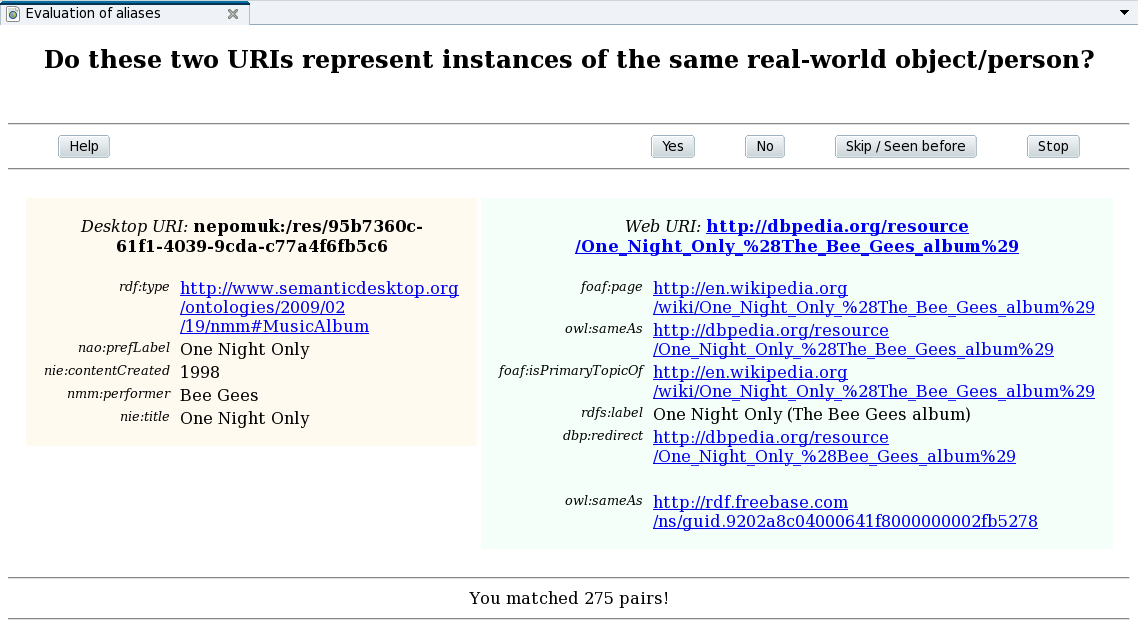
\includegraphics[width=\linewidth]{chapters/core/img/eval_album.png}
\caption{The Web interface of the experiment for collecting relevance judgements.}
\label{fig:onlineexperiment}
\end{figure} 

There were only two decisions possible: \emph{Yes} or \emph{No}, with a \emph{Skip} option, in case of uncertainty. Once a pair was judged or skipped, another one was shown to the participant. The pairs were randomly chosen from the remaining set. To add a gamification element to the experiment, we kept count of the number of pairs judged by each participant, and displayed it on the page. We found that even such a small addition generated ad-hoc competition and made the dull task more interesting.

The results of the experiment show an average agreement and its standard deviation, computed with Fleiss's $\kappa$, of $0.638\pm0.214$, over all three types of entities, suggesting substantial agreement between annotators. Table~\ref{tab:agreementsdwod} shows the Fleiss's $\kappa$ and its standard deviation $\sigma$ per type, as well as the average pairwise percent agreement. We observed that for music albums, there was only moderate agreement between annotators, visibly lower than the average, while for publications it is visibly higher. We believe the difference is caused by the fact that the data about publications is generated and curated by experts in the field --- even more so, as the publications were largely from the domain of Semantic Web --- while the music data comes from much more heterogeneous sources.

\begin{table}
\centering
\ra{1.3}
\begin{tabular}{@{}rcl@{\hs}l@{\hs}l@{}}
\toprule
& \phantom{a} & $\kappa$ & $\sigma$ & Avg  \\ 
\midrule

 All && 0.638 & 0.214 & 92.252 \\

 People && 0.661 & 0.257 & 88.2 \\

 Publications && 0.786 & 0.127 & 98.067  \\

 Albums && 0.442 & 0.233 & 90.523 \\

\bottomrule
\end{tabular}
\caption{Inter-annotator agreement measures}
\label{tab:agreementsdwod}
\end{table}

\subsection{Quantitative Results}

To evaluate the performance of the algorithm, we evaluate each of the matching parameters described in Section \ref{sub:matchingcomp}, activated either separately or using a combination of them, against a baseline which is the matching framework with all the parameters disabled. In the following, the String Matching parameter is denoted by SM, the Weighted Properties by WP and the Multi-Valued Properties by MVP.

We used the \emph{trec\_eval} tool\footnote{\url{http://trec.nist.gov/trec_eval/}} to compute standard information retrieval measures.
The precision at k ($P@k$) with k={1,2,3,4,5}, mean average precision (MAP) and normalised discounted cumulative gain (NDCG) are reported in Table~\ref{tab:agreement-albums} for music albums, Table~\ref{tab:agreement-people} for people and Table~\ref{tab:agreement-publications} for publications. 
We report also the interpolated precision at recall cut-off points when all matching parameters are enabled. The goal for the system is high precision, i.e., achieving a maximum at P@1. Recall is not a target, as it is generally impossible to determine the entire set of correct results available in the Web of Data.

\begin{table}[htb]
\centering
\ra{1.3}
\begin{tabular}{@{}rcl@{\hs}l@{\hs}l@{\hs}l@{\hs}l@{\hs}l@{\hs}l@{}}
\toprule
& \phantom{a} & MAP & NDCG & P@1 & P@2 & P@3 & P@4 & P@5 \\ 
\midrule

 SM WP MVP && 0.2464 & 0.5117 & 1 & 0.625 & 0.4167 & 0.3125 & 0.25 \\ %111

 SM WP && 0.2464 & 0.5117 & 1 & 0.625 & 0.4167 & 0.3125 & 0.25 \\ %110

 SM MVP && 0.2464 & 0.5117 & 1 & 0.625 & 0.4167 & 0.3125 & 0.25 \\ %101

 WP MVP && 0 & 0 & 0 & 0 & 0 & 0 & 0 \\ %011

 SM && 0.2464 & 0.5117 & 1 & 0.625 & 0.4167 & 0.3125 & 0.25 \\ %100

 WP && 0 & 0 & 0 & 0 & 0 & 0 & 0 \\ %010

 MVP && 0 & 0 & 0 & 0 & 0 & 0 & 0 \\ %001

 Baseline && 0 & 0 & 0 & 0 & 0 & 0 & 0 \\ %000

\bottomrule
\end{tabular}
\caption{Evaluation results for albums, when varying configuration parameters.}
\label{tab:agreement-albums}
\end{table}

In Table~\ref{tab:agreement-albums}, we can observe that only the SM parameter is enhancing the results compared to the baseline. The other two parameters do not improve the results at matching certain candidates. Also, in term of MAP and NDCG, the system achieves the lowest performance on the albums corpus. This can be explained by the fact that the Web resources returned by the query module for albums are mostly e-commerce products, which are not defined as a type of interest, and therefore are rejected by the matching module. However, some of the annotators have considered that the corresponding candidates are indeed the same as the album, while some have disagreed --- this is reflected in the agreement measure, as for the albums we have the lowest value for Fleiss's $\kappa$. Whether or not such candidates should have been kept by the system is open to discussion and left for future work.

\begin{table}[htb]
\centering
\ra{1.3}
\begin{tabular}{@{}rcl@{\hs}l@{\hs}l@{\hs}l@{\hs}l@{\hs}l@{\hs}l@{}}
\toprule
& \phantom{a} & MAP & NDCG & P@1 & P@2 & P@3 & P@4 & P@5 \\ 
\midrule

 SM WP MVP && 0.4212 & 0.6354 & 0.9302 & 0.8953 & 0.7597 & 0.6337 & 0.5442 \\ %111

 SM WP && 0.4174 & 0.6321 & 0.9286 & 0.8929 & 0.746 & 0.6131 & 0.5286 \\ %110

 SM MVP && 0.4212 & 0.6354 & 0.9302 & 0.8953 & 0.7597 & 0.6337 & 0.5442 \\ %101

 WP MVP && 0.2916 & 0.5338 & 1 & 0.8243 & 0.6036 & 0.473 & 0.3838 \\ %011

 SM && 0.4212 & 0.6354 & 0.9302 & 0.8953 & 0.7597 & 0.6337 & 0.5442 \\ %100

 WP && 0.2916 & 0.5338 & 1 & 0.8243 & 0.6036 & 0.473 & 0.3838 \\ %010

 MVP && 0.2877 & 0.53 & 1 & 0.8243 & 0.6036 & 0.4662 & 0.3784 \\ %001

 Baseline && 0.2877 & 0.53 & 1 & 0.8243 & 0.6036 & 0.4662 & 0.3784 \\ %000

\bottomrule
\end{tabular}
\caption{Evaluation results for people, when varying configuration parameters.}
\label{tab:agreement-people}
\end{table}

In Table~\ref{tab:agreement-people}, we can observe that the baseline, the WP and the MVP parameters are each able to match good candidates with high precision at P@1, with WP providing slightly better MAP and NDCG. However, the system does not get significant advantage by combining them. The SM parameter alone provides slightly lower precision at P@1 but significantly better MAP and NDCG. By combining the three parameters, the system does not get significant advantage and it seems that using SM prevails. 

\begin{table}[htb]
\centering
\ra{1.3}
\begin{tabular}{@{}rcl@{\hs}l@{\hs}l@{\hs}l@{\hs}l@{\hs}l@{\hs}l@{}}
\toprule
& \phantom{a} & MAP & NDCG & P@1 & P@2 & P@3 & P@4 & P@5 \\ 
\midrule

 SM WP MVP && 0.7773 & 0.8651 & 1 & 0.625 & 0.4167 & 0.3125 & 0.25 \\ %111

 SM WP && 0.8032 & 0.8609 & 0.9062 & 0.5781 & 0.3958 & 0.3047 & 0.2438 \\ %110

 SM MVP && 0.7175 & 0.7986 & 0.9231 & 0.5769 & 0.3846 & 0.2885 & 0.2308 \\ %101

 WP MVP && 1 & 1 & 1 & 0.5 & 0.3333 & 0.25 & 0.2 \\ %011

 SM && 0.7265 & 0.7883 & 0.8235 & 0.5294 & 0.3627 & 0.2868 & 0.2294 \\ %100

 WP && 0.6893 & 0.7347 & 1 & 0.55 & 0.3667 & 0.275 & 0.22 \\ %010

 MVP && 0 & 0 & 0 & 0 & 0 & 0 & 0 \\ %001

 Baseline && 0.7175 & 0.7588 & 1 & 0.5455 & 0.3636 & 0.2727 & 0.2182 \\ %000

\bottomrule
\end{tabular}
\caption{Evaluation results for publications, when varying configuration parameters.}
\label{tab:agreement-publications}
\end{table}

In Table~\ref{tab:agreement-publications}, the baseline provides good results from the start for publications. The system is not able to return any candidates when MVP alone is activated. However, when WP and MVP are combined, the system achieves much better results (in term of MAP and NDCG) than the baseline or than the WP parameter alone. When the system combines SM with the two previous ones, the system achieves a lower MAP and NDCG but an improved precision with a larger cut-off rank. While on the two previous types of entities, the SM parameter seemed to be the most important matching feature, this corpus shows that the WP and MVP are important matching features in certain cases.

\begin{figure}[htb]
 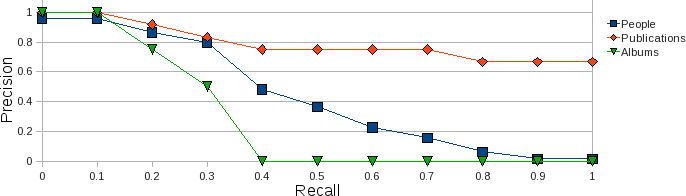
\includegraphics[width=\linewidth]{chapters/core/img/precrecal_wlabels.png}
\caption{Interpolated precision at recall cut-off points.}
\label{fig:precrecall}
\end{figure}

Overall, the results are satisfying for our use cases where high precision prevails over recall. However, given the results shown in Figure~\ref{fig:precrecall}, we can see that the system could be configured to return more than one entity in order to achieve better recall while keeping good precision. It might prove useful to implement a semi-automatic system which presents the top \emph{n} candidates to the user for manual selection.

\subsection{Performance}

To determine the performance, we measured the time spent on each step of the algorithm. We note that these results come from a prototype implementation, still to be subject to technical optimisations. Table~\ref{tab:sdwodtimes} shows the average times overall, and for each resource type separately, when all three parameters (SM, WP, MVP) are active. We find only small variations in the measurements when the parameter values are changed. We do not consider the time spent on retrieving data from Sindice, as this depends on external factors, like network speed and server availability. 

\begin{table}[htb]
\centering
\ra{1.3}
\begin{tabular}{@{}rcr@{\hs}r@{\hs}r@{\hs}r@{}}
\toprule
& \phantom{a} & Overall & People & Publications & Albums \\ 
\midrule

 Pair total && 375.04 & 52.19 & 977.87 & 53.18 \\

 Types check && 0.23 & 0.26 & 0.21 & 0.23 \\

 Per property check && 6.66 & 0.92 & 13.2 & 22.06 \\

 All properties && 2026.22 & 7.17 & 5478.87 & 1963.88 \\

\bottomrule
\end{tabular}
\caption{Time performance (milliseconds).}
\label{tab:sdwodtimes}
\end{table}

The checking of types is the only value that on average does not depend on the type of resource, as it must be performed for all pairs. The time spent in average per property check is low, but it varies by type, and by the complexity of the properties (e.g. it takes longer if several resources in the graph must be traversed, for long property paths like the name of the artist of an album). The ``All properties'' row shows the average time required for checking all the properties of an entity, and the computation of the final score\footnote{The ``All properties'' row has values higher that the ``Pair total'' row because the average time is computed only for those pairs that passed the type check, thus fewer, but with longer computation times.}. These values depend on the type of resources as well, and on the complexity of the resource graph. We found that longer times correspond to very big graphs for online entities, which must be loaded for checking even if in most cases are not found to represent valid 
candidates\footnote{e.g., the graph for \url{http://webconf.rkbexplorer.com/models/iswc-aswc-2007-complete.
rdf}}.


\section{Discussion}

The scope of the system presented here is limited to finding Web of Data aliases for desktop resources. We leave the use of the aliases found to future work, but the use cases include personalised desktop services like those described in Section~\ref{sec:sdwodintro} and enhancement of desktop information from online sources like the one described in \cite{Groza2009}. We plan to develop a semi-automatic service that retrieves information from the Web aliases and updates the local resources, while saving provenance information for the imported data and allowing synchronisation when the Web data changes.

Existing Web applications already provide similar services via specific APIs (e.g., last.fm). However this is not the goal of our work. Instead, we wish to leverage information across all public information sources accessible on the Web of Data. In addition, such third-party APIs are seen as an additional information sources on the Web, and are supported by our system.

Within the system, we make use of existing semantic technologies, including semantic search engines such as Sindice. In the process of determining the aliases we focus on selecting the most appropriate URI from the list of candidates returned by the search engine. In this case, the issue of which data sources to trust is left to the search engine, which usually employs advanced techniques~\cite{Delbru2010} for making the decision. This is however not a requirement we impose on the users, who can choose to query other trusted data sources suitable for their use case.

The system we presented is automatic, as no user interaction is required for it to work. Once set up it will find and save aliases to desktop resources. 
Although the mappings were created manually, they are part of the system and do not need to be modified by end users. 
Power users can however tweak the settings to fit their specific needs by enabling or disabling modules, changing threshold values or modifying mappings.
While new mappings can only be created manually, expert users can take advantage of the openness resulting from the use of SPARQL-based search mechanism and update the mappings as they need, or create new ones. We envision for the future, a way of allowing power users to publish their own mappings and let other users install new mappings in a way similar to installing add-ons to Web browsers.


\section{Conclusion}

In this chapter, we presented a framework to automatically link entities from the Semantic Desktop to the Web of Data. This is the logical next step after the creation of semantic data on the desktop, presented in the previous chapter.

The framework uses existing technologies such as semantic search engines and public SPARQL endpoints for retrieving a set of candidates. Each candidate is then evaluated more precisely based on a collection of matching components using string matching, heuristics and rule-based mechanisms. We evaluate the system qualitatively, using real-world data retrieved from a Nepomuk-KDE Semantic Desktop and the Sindice search engine. The evaluation is based on relevance judgements from a group of experts. We show that the system in its current form provides satisfactory results in term of precision for automatic linking of entities.

Once the two networks of linked data are connected, we can build semantic applications and services using personal data from the desktop and enriched with information from the Web of Data. In the next chapter we present one such application.


\chapter{Transforming Semantic Notes into Semantic Blog Posts}
\label{ch:semblogging}

\begin{flushright}
 \textit{Based on ``Linking Semantic Personal Notes'' \cite{Dragan2010a}\\published at the Workshop on Knowledge Injection into and Extraction from Linked Data (KIELD~2010~co-located~with~EKAW~2010)}
\end{flushright}

In the previous two chapters we showed how Semantic Web technologies are available both on the desktop and of course on the Web, and how the two networks of linked data can be connected. SemNotes, a semantic note-taking tool for the Semantic Desktop, described in Chapter \ref{ch:semnotes}, shows how new data can be created and seamlessly integrated with existing semantic information from the desktop. Chapter \ref{ch:sdwod} describes an algorithm for automatically connecting desktop resources to their Web aliases, bridging the gap between the desktop and the Web in regards of semantic data, opening up the possibility of augmenting desktop data and building personalised desktop services. 

In this chapter we present a use case, and a proof of concept system which builds on our previous work in order to support easy publishing and sharing of semantic personal notes taken with SemNotes as Linked Data.
Our approach can be used to publish any kind of information from the desktop to the Web, enabling integration of small chunks of personal knowledge into the Web of Data.
This use case illustrates a solution to the second research question \textbf{Q 2.} from Section \ref{sub:question}, \emph{How to expand the scope of the Semantic Desktop into the realm of the Web of Data, to enhance the user experience and benefit?}, more specifically, to the second and third sub-questions \textbf{Q 2.2.} --- \emph{How to use the Web information found related to a desktop resource?}, and \textbf{Q 2.3.} --- \emph{How to make desktop data available online safely?}

\section{Introduction}
\label{sec:introduction}

Semantic Web technologies are deployed in various domains and applications, both on the desktop and on the Web.
While these two domains share compatible representation models (RDF(S)/OWL), there is still a gap between data from the Web and the desktop. We showed in the previous chapter how finding Web aliases for Semantic Desktop resources enables us to bridge this gap. This solution is however unidirectional --- it only solves connection from the desktop to the Web, and not the reverse, from the Web to the desktop. It can be argued that accessing desktop information from the Web is not necessary, or not safe, or that the risks exceed the benefits. However, sharing desktop information online has many possible use cases, and does not necessarily involve making private information public. 

One such use case of sharing desktop information and realising better integration of personal data with online data, is described in this chapter. We present an approach for publishing personal notes from the desktop (using SemNotes and Semantic Desktop technologies) to the Web of Data (using the Linked Data principles). Our goal is to publish this data online without losing the personal context established on the desktop through the links from the notes and the related desktop resources.
Our approach consists of two main steps: 
\begin{enumerate}
 \item preparing the desktop data for sharing, 
 \item publishing it online. 
\end{enumerate}
In addition, it requires two prerequisite steps, which are supported by previous work: 
\begin{itemize} 
 \item the note-taking process and annotation of the note (adding the context) which was presented in Chapter \ref{ch:semnotes}, and 
 \item the identification of Web URIs which represent the same real-world thing as the desktop resources that belong to the context of a note, which was presented in Chapter \ref{ch:sdwod}. 
\end{itemize}

Our contribution consists of the process for publishing personal information from the desktop to the Web following the Linked Data principles \cite{BernersLee2006}, and a system implementation that allows sharing of semantic personal notes as semantic blog posts, interlinked with existing information from the Web of Data. 
The publication process must follow the Linked Data principles, while at the same time protecting sensitive private data from being shared unwillingly, and maintaining the meaningful relations in the process.


The semantic notes taken with SemNotes constitute the personal information that we want to publish as Linked Data. They are semantically linked to local resources mentioned in their content, like people, projects or other notes. If the notes were directly published online, the relations that enrich them would be lost and the links they contain would be broken, because they point to local URIs not available outside of the desktop. The same objects often exist within the Web of Data, therefore the note links to them can be recreated in the publishing process. Before the note is published, our system searches for existing public Web aliases for the local resources. They are then used to substitute the local private data referenced in the text --- the links are changed to point to the Web resource. In this way, the published links are valid, the meaning of the link is preserved (as referring to the same entity) and the private information is protected. The system then publishes the notes online as blog posts 
taking care of the transformations required from desktop ontologies to Web ones, according to the mappings devised in Chapter \ref{ch:sdwod}.

In line with the two-step process mentioned above, our system has two modules, one working on the desktop and the second one online. First, the desktop part handles the preparation of the notes for publishing, using the Web aliases identified by the service described in the previous chapter, substituting them for the local ones, as well as the transformation required from desktop ontologies to Web ones. This module is invisible to the user, except for the \emph{Publish} button shown in the user interface of SemNotes. Then, the Web part publishes the transformed notes as Linked Data in accordance with the Linked Data publishing principles.

The solutions provided by most existing systems fall into two categories: \begin{inparaenum}[(i)] \item desktop applications that involve publishing the actual local resource information together with the note, or \item online applications that do not have access to desktop data relevant to the user. \end{inparaenum} The first category, represented by tools like SemiBlog \cite{Moeller2005} or SemBlog \cite{Takeda2005}, is not optimal when dealing with resources that contain sensitive private information. Services like Zemanta\footnote{\url{http://www.zemanta.com}}, from the second category, have access to various online resources, but not to the personal context of the user.
Also they miss the personal touch of desktop-based applications.


\section{From Note-Taking to Weblogging}
\label{sec:reqsemblog}

Two characteristics of blog posts which are relevant to this use case are: 
\begin{itemize}
 \item their topics are of interest to the author and thus are very likely to have references to things also present on the desktop (e.g. people, events); 
 \item the context consists of the references made in their content, such as places, projects, or other blog posts.
\end{itemize}

However, not all blog posts start by being a blog post. Some are just ideas or impressions jotted down for later, in one's preferred desktop note-taking application. Nevertheless, some of these notes do become posts after polishing and refining, especially as some notes might require further investigation before they can be published (e.g. when writing on a technical subject). Examples include notes taken at presentations, ideas on topics of interest written down at times when blogging is not possible (attending a meeting or lack of Internet connection).

Tools from the Semantic Desktop, like SemNotes, provide means to enhance these notes locally, by interlinking them with other desktop data --- the contacts in the address book, the events from the calendar application, the projects worked on, the music listened to. 
For example, a note about an upcoming concert can be linked to the performing artist which is in turn linked to the music files of that artist and pictures from earlier shows stored in a desktop photo application.
Such annotations give context to the note and should be preserved when the note is published as a blog post on the Web, since it enables serendipitous browsing and information discovery, through the relevant additional links they contain.

Currently, personal notes, even the ones semantically enriched using Semantic Desktop applications, must be published as blog posts by being manually copied into a blogging tool.
In this way, any additional semantic information available on the desktop is lost or, if copied, leads to broken references as they point to the local resources which are not accessible outside of the desktop.
The note-taking to publishing process is sometimes cut short by using the drafting functionality offered by some systems like WordPress or Blogger, so that users can directly take the notes in the blogging tool, usually online, thus replacing the desktop note-taking application completely. However, using online tools deprives the user from having the personal context added to the blog post, since desktop information cannot be easily integrated in Web-based services.

In order to enable a better transition from personal notes to blog posts, or simply to Web-based information available to others (for example, meeting notes published in a company intranet or lecture notes shared between students of the same class), we defined a list of requirements that a system for publishing semantic personal data online should fulfil:
\begin{description}
 \item[R1.] Publish the complete desktop data on the Web without losing any relevant information, including metadata and context (e.g. tags, relations, identifiers);
 \item[R2.] Protect any machine readable and private data that might be unwillingly included in the context being transferred\footnote{The protected data does not include the actual text to be shared as it is a conscious decision to publish it, taken explicitly by the user};
 \item[R3.] Publish the note according to the Linked Data principles and describe it using popular ontologies; 
 \item[R4.] Enable object-centred sociality by establishing connections between data published by different users.
\end{description}


\section{Overview of the Process and Prerequisite Steps}
\label{sec:sembloggingapproach}

We propose an approach that enables the publishing and sharing of personal notes by extending the functionality provided by SemNotes, and by using the Web of Data aliases found for desktop resources. The process consists of two steps: 
\begin{enumerate} 
 \item transformation, and 
 \item publication. 
\end{enumerate}
In the first step, the note is transformed locally for publication, and private local data is replaced with public references.
In the second step, the transformed note is published online.

The system requires a dedicated server, where the resources referenced and the tags assigned are shared between the notes of all users, to add a social aspect. Also, rather than trying to determine which of the many possible Web aliases found for a desktop resource is authoritative, we let the server create equivalent public resources and connect all the aliases to them. We also used the server for publishing the notes, although this can be replaced by any other blogging platform.

The first prerequisite step --- note-taking and annotation of the note with the relevant desktop resources --- must be performed before any actual sharing of notes can be done. The annotation is done semi-automatically and is an existing feature in SemNotes. 

The second prerequisite step consists in finding Web resource for each of the desktop entity linked to the note that is about to be published. This step is executed by a desktop service which implements the two-part algorithm detailed in the previous chapter, the blocking pass using Sindice to retrieve possible candidates and filtering the list by the score returned by the matching algorithm. The local service has access to, and uses all the information available on the desktop about a resource to identify only exact matches for it. The aliases which are found for the desktop resources are saved by creating a \verb|pimo:hasOtherRepresentation| link in the local repository between the desktop resource and the Web one.


\section{System Implementation Details}
\label{sec:sembloggingsystem}

Based on the process described above, the system is divided between its local part and its remote part, as shown in Figure \ref{fig:semblogsystem}. The local part handles local \emph{private} data, while the remote one handles online \emph{public} data. 
\begin{figure}[htb]
  \begin{center}
    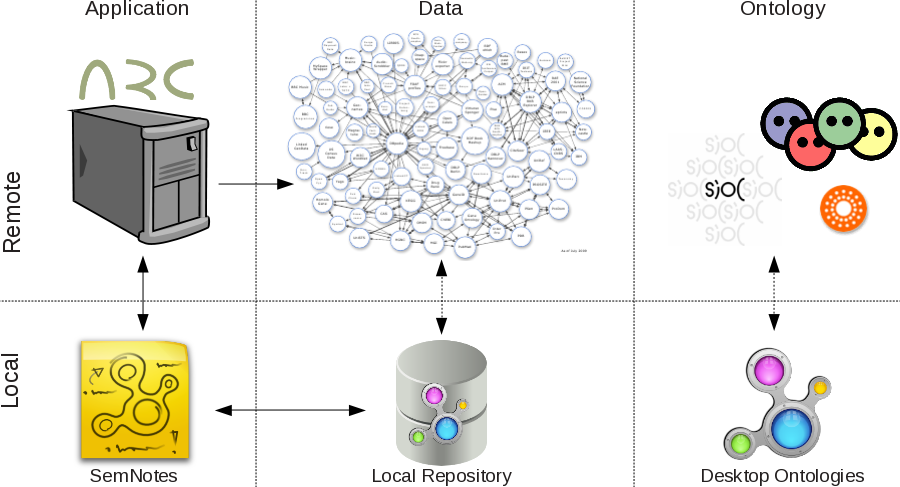
\includegraphics[width=0.8\linewidth]{chapters/core/img/system}
    \caption{Overview of the semantic publishing system.}
    \label{fig:semblogsystem}
  \end{center}
\end{figure}
The separation between them extends over three layers: ontology, data and application.
On the \emph{ontology} layer, the NEPOMUK desktop ontologies are used locally, while popular Web vocabularies are used on the server-side. These ontologies are used to describe the \emph{data} exchanged between the applications. Desktop data is stored in the local NEPOMUK repository, while Web data is distributed. Finally, on the \emph{application} layer, the local component is an extension to SemNotes that provides publishing functionality for notes, and the remote component is a server that hosts and publishes online the notes received.

The first step of the process --- transformation --- is executed on the local side, by an extension of the SemNotes application. Then, the publication step is done by the server, which receives information from the desktop and publishes the note, as we will describe next. The two application components, the communication between them, and the data translation process are described in detail below.

\input{chapters/core/sempub/ontologies}

\input{chapters/core/sempub/schema}

\input{chapters/core/sempub/transformation}

\input{chapters/core/sempub/publication}

\section{Conformance with the Initial Requirements}
\label{sec:evaluationsemblog}

When establishing the specifications of the framework, we identified four main requirements (Section \ref{sec:reqsemblog}).
Our proposed implementation conforms with them as follows.

\emph{\textbf{R1}: Publish the complete desktop data on the Web without losing any relevant information, including metadata and context (e.g. tags, relations, identifiers).}\\
By translating existing desktop data surrounding the note to RDF and putting it online, available as RDFa, the entire information available on the desktop side is made available on the Web for further reuse.
In addition, all information from the original note-taking tool, including title, tags, etc. is publicly made available on the Web.

\emph{\textbf{R2}: Protect any machine readable and private data that might be unwillingly included in the context being transferred;.}\\
By replacing the private desktop data with equivalent public Web data, we protect the former. On the desktop there is a lot of private information stored about resources, like the email address or telephone number for people, or the list of attendees of an event. When the person or event is linked to a note that is afterwards published online, such private information is not exported, because the reference to the local resource is replaced by a reference to already public Web data representing the same thing. In this manner, the context of the note being published is preserved, but the private details are not exposed.

\emph{\textbf{R3}: Publish the note according to the Linked Data principles and describe it using popular ontologies.}\\
Our system publishes notes on the Web using the Linked Data principles. Each note and connected resource, has its own URI, which is made dereferenceable, while distinguishing information resources and non-information resources.
In addition, while original desktop data is provided using ``desktop ontologies'', the published information is made available using FOAF, SIOC, Dublin Core, etc. and the mappings have been validated through Vapour\footnote{\url{http://vapour.sourceforge.net/}}.

\emph{\textbf{R4}: Enable object-centred sociality by establishing connections between data published by different users.}\\
Since resources and tags are shared between users, notes can be browsed serendipitously through shared connections, or tags. 
This enables ``object-centred sociality'' \cite{KnorrCetina1997}, since people can interact around these shared tags and topics, such as projects or people that they have in common.
Depending on the destination of the publishing process, there is the possibility of having private notes, yet still accessible online by registered users only.


\section{Related Work}
\label{sec:relatedworksemblog}

Semantic blogging was introduced by \cite{Cayzer2003}, and since then has received much interest. Later \cite{Karger2004} described semantic blogging in the context of the Semantic Web with Haystack. So far, existing systems for semantic blogging fall into two categories: 
\begin{itemize}
 \item desktop applications that involve publishing the actual local resource information together with the blog post, or
 \item online applications that do not have access to desktop data relevant to the user. 
\end{itemize}

The tools in the first category, like SemBlog \cite{Takeda2005} and SemiBlog \cite{Moeller2005}, have the advantage that users have better access to the relevant data from the desktop. However, both tools require that the resources that contain sensitive private information are published together with the blog posts, which might lead to privacy issues. The SemBlog project allows users to add data from personal ontologies to their blogs. SemiBlog allows integration of personal data in the posts by drag and drop from various desktop applications like the address book. SemBlog and SemiBlog are used for exchange of personal information in the blog posts, which differs from our approach of using already published Web data as to protect the privacy of the personal information. SemiBlog's process implies manually adding the metadata, while our approach relies on automatic export. Both tools comply with our first requirement, but not with the last three.

Online services like BlogAccord \cite{Cayzer2006} for music information, and Zemanta\footnote{\url{http://www.zemanta.com}} blogging assistant, belong to the second category. They have access to various online resources to create the context of a blog post and enhance the blogging experience, but they do not use the personal context of the user.



\section{Conclusion}

In this chapter we presented an approach for publishing semantic information from the desktop as Linked Data on the Web. The approach is realised by a system which takes semantic notes from the desktop and makes them part of the Web of Data, as semantic blog posts. The goal of the system is to provide a way for publishing and sharing complete information by preserving the personal context of the notes without compromising privacy. While the use case presented is focused on notes and semantic blogging, the same approach can be applied to publishing of any interlinked information. 

We defined a publishing process that comprises of two steps:
\begin{enumerate}
 \item preparation --- the note is transformed into a SIOC-based Web representation; and
 \item publication and sharing --- the note is published online following the Linked Data principles.
\end{enumerate}

In addition, we provided an implementation of the process, and tested it against a set of requirements regarding publishing personal content from the desktop to the Web as Linked Data.

While we do not authentication issues in this current release, we are considering SW-compliant systems such as FOAF+SSL \cite{Story2009} for future versions of the system.
We also plan to develop additional integration modules for publishing platforms, e.g. Drupal, WordPress, and to investigate approaches for authentication and notification tailored towards the people mentioned in the published data.


\chapter{Additional Extensions and Applications}
\label{ch:mischelperapps}

In this chapter we describe several applications developed in our SmILE\footnote{\url{http://smile.deri.ie}} group at DERI, and to which we contributed. They are extensions to the work presented in the preceding pages, providing or serving as test use cases and validation scenarios.

We start with a list of extensions to SemNotes' functionality, which employ Natural Language Processing techniques. They focus on specific use cases of note-taking, like ontology engineering, meeting minutes or status reports; as well as text analytics tailored to short text.

The work presented in Chapter \ref{ch:sdwod} was initially motivated by the increasingly difficult task of managing publications on the desktop and on the Web, and the need of connecting the information available in both worlds. \emph{Sclippy} is a tool created to avail of the rich information available on the Web about publications, and bring it to the user's desktop. 
The algorithm described in Chapter \ref{ch:sdwod} is a generalisation of the algorithms used in Sclippy\footnote{\url{http://smile.deri.ie/projects/sclippy}}, extending the scope from publications to any type of desktop resources.

We continue by presenting Konduit, a desktop-based platform for visual scripting with RDF data. Based on the idea of the Semantic Desktop, non-technical users can create, manipulate and mash-up RDF data with Konduit, and thus generate simple applications or workflows, which are aimed to simplify their everyday work by automating repetitive tasks. The platform allows to combine data from both the Web and the desktop and integrate it with existing desktop functionality.

\section{Natural Language Extensions for SemNotes}
\label{sec:nlpsemnotes}

During its development phases, SemNotes has served as a sandbox environment and testing bench for several technologies and prototypes developed within our group. Three of the most notable extensions are related to Natural Language Processing (NLP) of the notes, to add functionality. These include: 
\begin{itemize}
 \item a text analytics extension for keyphrase extraction \cite{Schutz2008}
 \item two controlled language extensions for semantic annotation of meeting minutes and status reports \cite{Davis2008,Davis2009}
\end{itemize}

\subsection{Keyphrase Extraction}

Tagging is one of the most used basic features offered by Nepomuk-KDE and by SemNotes. Tags are important for categorisation and organisation of resources, especially for personal notes. Tagging requires users to make a decision on what is relevant about the resource being tagged and how they might reuse the annotation in the future --- i.e. is the tag expressive enough to be later user for filtering the information and finding the required resource. To support users in their choice of tags, and partially automate it, we collaborated on a keyphrase extraction extension to SemNotes. It is based on the TextAnalytics service developed by \cite{Schutz2008}. 

Keyphrase extraction is just one of the NLP functionalities provided by the Text\-Analytics desktop service, alongside information extraction and speech act detection. The service can be accessed by all desktop applications and is available also as an Eclipse plugin for the Java implementation of Nepomuk.

Standard information extraction tools usually extract information which is already known --- like detecting resources in the text. This is the norm in SemNotes as well, where only known existing desktop resources are suggested as annotations of notes, even when other resources might be referred to, but are unknown to the system. The TextAnalytics service is different and complementary, by extracting terms and instances from text, which are not already known to the system. The new terms can become new desktop resources, once identified.

\begin{figure}[tb]
 \centering
 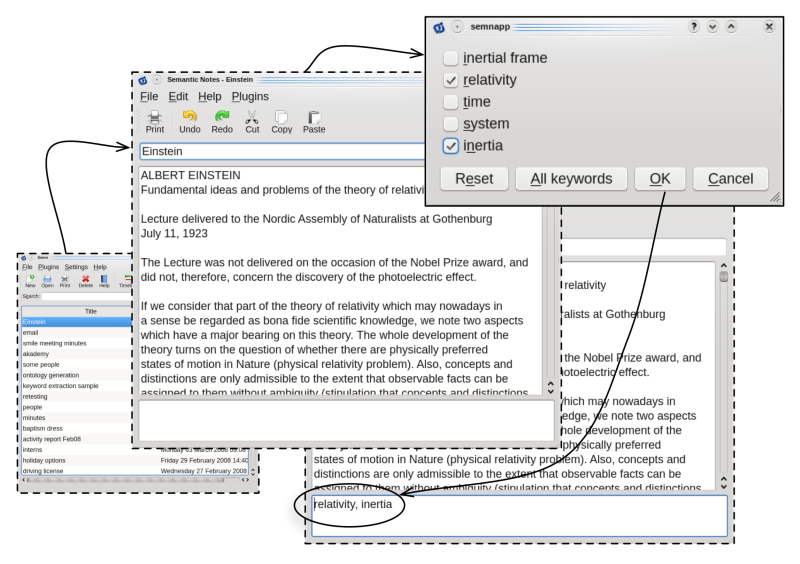
\includegraphics[width=\linewidth]{chapters/core/img/keywordextraction}
 \caption{User interface to keyphrase extraction in SemNotes.}
 \label{fig:keywordextraction}
\end{figure}

We have developed an extension to SemNotes, which uses the service to extract keyphrases from the text of the personal notes and suggest them to the user as tags. The text of personal notes can be small, thus adding difficulty to the extraction task. \cite{Schutz2008} details the way this challenge is tackled in the service. In SemNotes, the service can be called through the menu, and once the note is parsed the relevant terms found are presented to the user as tag suggestions. Figure \ref{fig:keywordextraction}, taken from \cite{Schutz2008}, shows a screenshot of the interface in an older version of SemNotes. If the user accepts any of the suggestions, they become tag resources and are stored in Nepomuk in the usual way.

\subsection{Controlled Language Extensions}

Controlled Natural Languages are well-defined subsets of a natural language with a restricted grammar and lexicon \cite{Schwitter2005}, in order to reduce ambiguity and complexity. In his Ph.D. thesis \cite{Davis2012PhD}, researches the use of Controlled Languages for ontology engineering and semantic annotation. We used SemNotes for prototype testing of both directions, while also providing a feasible use case for the services.

SemNotes, as a note-taking application, is well suited for Controlled Language use, since the main type of input from the users is textual. As a Semantic Desktop application it is also particularly well suited to ontology engineering due to the direct access provided by the framework to the underlying ontologies and desktop resources. As an annotation tool it is also a good testing ground for the semantic annotation using Controlled Language.

\subsubsection{Round Trip Ontology Authoring}

Controlled Natural Language proved efficient for creating ontologies in a user friendly way, for naive users who do not wish or do not need to learn how to use full-fledged ontology editors, nor want to dive into the complexities of ontology engineering. However simplified, Controlled Languages still require that the users be familiar with the vocabulary and syntax rules in order to use the language properly. The Round-trip Ontology Authoring environment described in \cite{Davis2008} aims to reduce the learning curve required to use Controlled Languages for ontology authoring. It combines and builds on the CLOnE controlled language for ontology editing \cite{Funk2007}, and Natural Language Generation from existing ontologies, to provide a simplified process: starting with an existing ontology, either imported or produced using CLOnE, generate the Controlled Language, edit the text, then parse it back into the modified ontology. Since the user only has to work with the textual representation of the ontology, we created a prototype extension for SemNotes to test the process.

Our extension allowed all the steps of the process --- import of existing ontologies, editing and exporting back into an ontology. It also had the added benefit of having access to all the ontologies loaded on the Semantic Desktop, and all the instances extracted from the personal data available on the desktop. Thus SemNotes allowed reuse of existing instances from the desktop in the ontology editing, and more importantly to create instances directly into the desktop repository, in a simple and user friendly way. It also meant that through this extension we could provide a way of easily creating or removing a relation between existing instances just by typing a sentence about it. 

\subsubsection{Controlled Language Annotation}

As we described before, SemNotes provides semi-automatic annotation of notes, by checking the available desktop resources and suggesting instances which are relevant to the note. Semi-automatic annotation is a mechanism often used to simplify the process of semantic annotation, and support the user. By employing Controlled Natural Language techniques, we can improve further the annotation process, in a user-friendly way. \cite{Davis2009} presents two approaches to applying Controlled Language to Semantic Annotation, called CLANN --- Controlled Language ANNotation. The two approaches were used to measure and evaluate the balance needed between expressiveness of the language and ease of use. CLANN is based on CLIE (Controlled Language for Information Extraction) and CLOnE. 

Semantic annotation with Controlled Language is better suited for some annotation scenarios than for others. CLANN is applied to two use cases, where the use of a controlled vocabulary is implicit --- meeting minutes and status reports. However, other possible use cases include the eHealth and business domains. The two use cases benefit from a semantic note-taking tool like SemNotes, thus creating an extension that uses CLANN was the next logical step.

The CLANN extension of SemNotes allows users to simultaneously create and annotate meeting minutes or status reports in Controlled Natural Language. It goes beyond the initial interlinking capabilities of SemNotes, by allowing the creation of different relations between the notes and desktop resources, as well as the creation of new resources and relations. CLANN uses a specially designed ontology for the meeting minutes and status reports, called MEMO, which is based on the desktop ontologies described in Section \ref{sub:nepomuk}. The notes must follow a specific template, which is then parsed by the service. In the parsing, the extension reuses SemNotes' mechanism for detecting related desktop resources. The information resulted from the parsed note is stored in the desktop repository.


\section{Linking Publication Data with Sclippy}

The work presented in Chapter \ref{ch:sdwod} is based on previous work \cite{Groza2009} on linking publication data from the Web of Data and from the Semantic Desktop. It consists of a three step process (extraction, expansion, integration) that starts from a file with no metadata and incrementally enrich it to a comprehensive semantic model around the given publication, linked and embedded within the personal information space. The process is implemented by Sclippy. 

The three steps are: 
\begin{itemize}
 \item extraction --- metadata is automatically extracted from the publication; 
 \item expansion --- the extracted metadata is used to search the Web of Data and find relevant information which is then connected to the original metadata; and 
 \item integration --- the metadata is further enriched by embedding it within the Semantic Desktop, where it is automatically linked with the existing personal metadata.
\end{itemize}

The work done by \cite{Groza2009a} is broader in a sense than our work, as it also includes in the first step of the process --- extraction --- containing complex algorithms for shallow (i.e. title, authors, abstract) and deep (i.e. discourse knowledge items like claims, positions or arguments) extraction of metadata from documents. Our work relies on the metadata already extracted by external applications or by the underlying Semantic Desktop, and instead focuses on the expansion and integration steps. We also aimed to provide a generic model for the integration of Web of Data sources and the Semantic Desktop, broadening the scope from the world of publications and authors.

The linking of publications done by Sclippy was motivated by the growing difficulty for early stage researchers to determine relevant work in a domain. The existing efforts are limited in the online world, where there are many publishers, each providing access to disjunct corpora of publications, and regardless of how well interconnected and easy to search they are, they do not cover all possible sources. The Semantic Desktop, being the implicit place where researchers would store documents, and already providing means of interlinking and better management of information, is the obvious choice for connecting to the similar but richer information available on the Web.

While Sclippy served as basis for our work, it also provided our first real-world use case where the interlinking of the Semantic Desktop data with the Web of Data would be useful, as well as the first example of a customised desktop service benefiting from it.


\section{Building User-Applications with Konduit}

An added benefit of structured information is its potential for reuse: being able to integrate existing data, relieves users from creating it again. While a large part of the data is found online, when it comes to working with information, users still rely on the familiar environment of desktop-based applications. On the other hand, Web-based applications can only access Web data, and do not integrate well with desktop information.

Konduit \cite{Dragan2009b} offers a way of accessing structured Web data from the desktop, integrating it with existing desktop data and applications, and working with both in a unified way. It precedes the system for finding Web aliases for semantic resources from the desktop, presented in Chapter \ref{ch:sdwod}. 

The goal of Konduit was to allow the users to easily design their own personalised applications, customised to their needs and based on their workflows, without requiring prior knowledge of programming languages, or even semantics.
Our approach with Konduit is based on a combination of the visual programming paradigm and the idea of UNIX pipes, and allows the casual users to build simple programs in order to perform and automate everyday tasks on RDF data. In other words, it is visual programming for RDF. 

\subsection{Components and Workflows}
\label{sec:konduit_components_and_workflows}

Konduit provides a collection of useful components ready for immediate use. The components offer individual units of functionality and are represented visually as blocks. They are connected through input and output slots, and in this way the flow of the program is defined. In order to keep simple the task of connecting components, the only data that flows through the workflow is RDF. This condition ensures that each component always fulfils the minimal requirement for dealing with its input. Obviously, components may be specialised with respect to the actual vocabulary on which they can operate and will decide at runtime if and how they deal with the incoming RDF. By neither allowing different kinds of data (e.g., text, numbers, lists, images, etc.), nor typing the RDF data with respect to the vocabularies they use, we stay very close to the original UNIX pipes concept, where data is always an untyped stream of bytes, and where it is up to each process or program how to handle it. 

The architecture of Konduit is modular, each component is realised as a plugin which can be independently installed or removed. We expect that new plugins will be developed and shared by external power users, as the need for them arises. 
Formally, a component is defined by the following parameters:
$$
Component = (I, O, P, F )
$$
\begin{itemize}
 \item a set of RDF input slots $I$,
 \item a set of RDF output slots $O$, 
 \item a set of parameters $P$ which allow for user input in the workflow, 
 \item a function $F$, which works on the input $I$ and generates the output $O$.
\end{itemize}
The parameters $P$ influence the behaviour of $F$.

The number of input and output slots is not fixed and can be 0 or more. Depending on the number of slots, components can be grouped in three categories: sources, sinks, and ordinary components. Sources are components that do not have any inputs. They supply the workflow with data. There is always at least one source at the start of any workflow. Because data graphs can be merged, there can be more than one source for any workflow. Typical examples of sources are connectors to RDF stores, file (URL) input components, or converters from other, non-RDF formats. Sinks are components that do not have any outputs. They represent the final point(s) of any workflow. Examples of sink components are application adaptors, serialisers (file output components) and visualisers. In Konduit, workflows are activated from a sink component, usually by clicking on an activation button.

Several connected components make up a workflow, which is defined by specifying
$$
Workflow = (C, f) , where f: inputs(C) \rightarrow outputs(C) \cup \{~nil~\}
$$
\begin{itemize}
 \item a set of components $C$,
 \item a function $f$ defined from the set of all the inputs of the components of $C$ to the set of all the outputs of the components of $C$ and the $nil$ output.
\end{itemize}
The function $f$ shows how the components of $C$ are connected. The inputs that are not connected have a $nil$ value of $f$; the outputs that do not represent a value of $f$ are not connected.

Workflows can be saved and reused. Saving a workflow implies saving all the components that have at least one connection to it, as well as their existing connections, parameters and layout. There is no restriction that the components should be completely connected, so there can be input or output slots that remain open. A saved workflow can be reopened and modified by adding to it or removing components, or by changing connection or parameters and thus obtaining different workflows with minimum effort.

An important aspect of Konduit is directly tied to the fact that all inputs and outputs are RDF graphs. As a result, any workflow can itself become a component, meaning that workflows can be built recursively. In this way, it is possible to create specialised components, which we call black boxes, based on the combination of other components. The blackboxes are added to the existing library for reuse. An example of saved workflows and blackboxes is shown in Figure \ref{fig:discography_generator}. The workflow is taken from \url{http://smile.deri.ie/konduit/discography}, where an entire example use case is presented.

\begin{figure}[!ht]
 \centering
 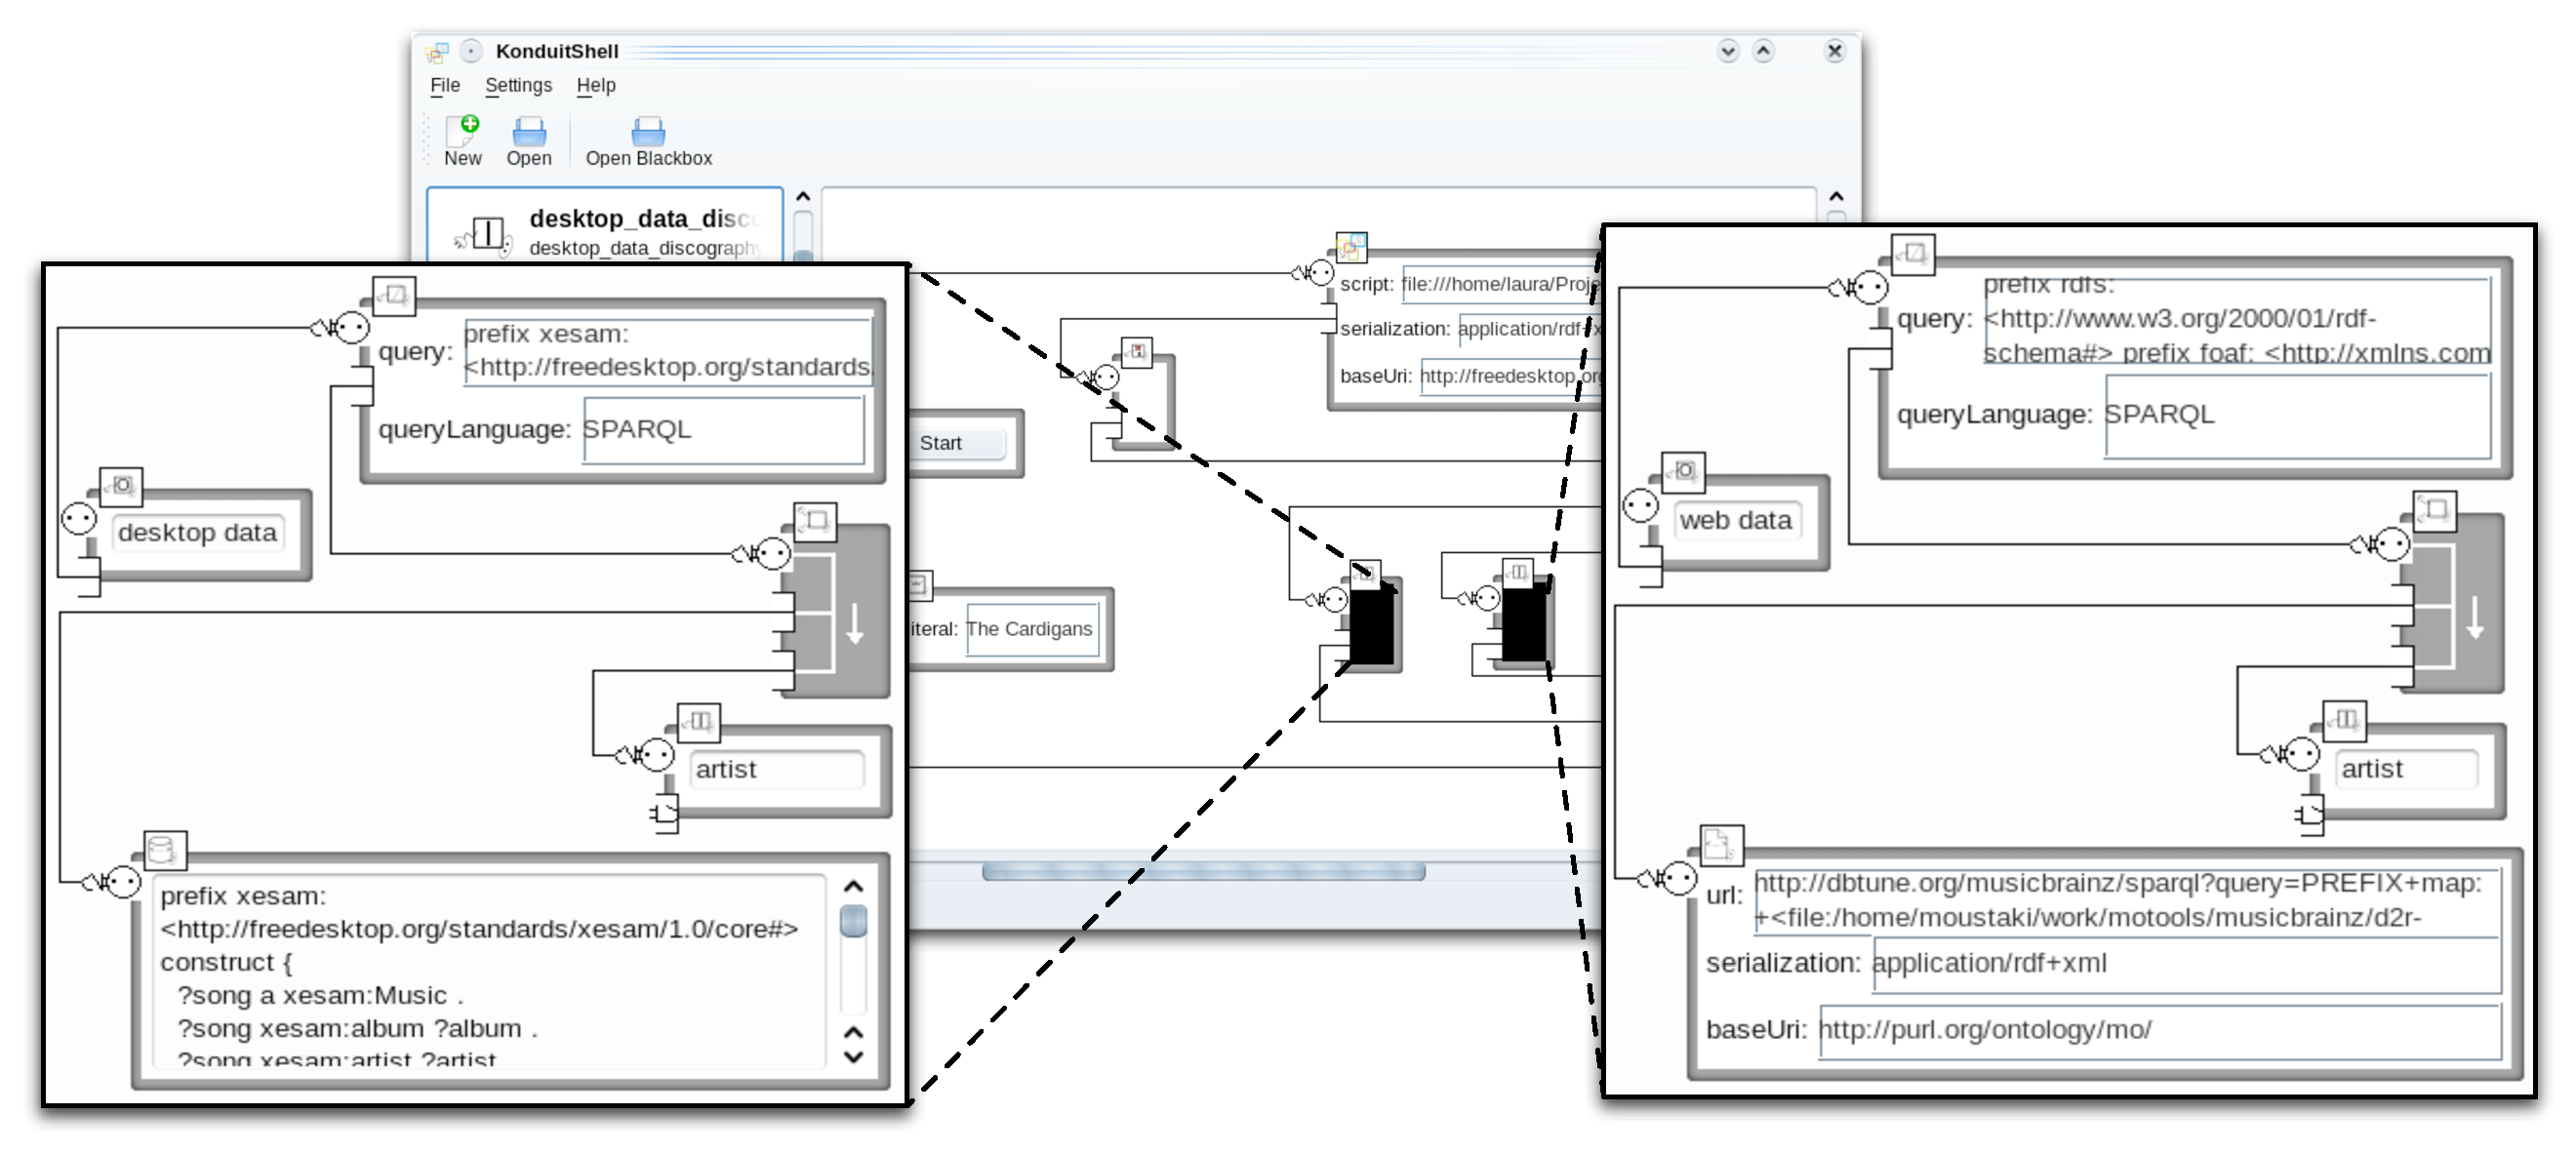
\includegraphics[width=1.0\linewidth]{chapters/core/img/discography}
 \caption{The entire discography generator workflow.}
 \label{fig:discography_generator}
\end{figure}

\cite{Dragan2009b} describes in more detail the different types of sources, sinks, and ordinary component types, as well as the blackbox mechanism. 
Some of the basic components available for Konduit require previous knowledge of writing SPARQL queries. Since the queries can influence the performance of the entire workflow, we recognise the need for a smart query editor that is suitable for naive users. \cite{Ambrus2010} describes the means for making Konduit more user friendly, by adding a smart wizard with suggestions and SPARQL autocompletion. 


 \part{Conclusion}
\label{part:conclusion}

\chapter{Conclusion and Outlook}
\label{ch:conclusion}

The Semantic Desktop is a framework for semantic interlinking of desktop data. We ground our work in it, using the building blocks it provides --- the foundations of data representation and the layered service oriented architecture ---, to enhance it further, through good user-facing semantic applications, and to connect it to the large source of Linked Data that is the Web.

The approach we took in this thesis is data-centric. We focused on maintaining and enriching the network of linked personal data that the Semantic Desktop enables. The path we took is two-fold, with both directions working towards interlinking semantic personal data. The first direction is internal, on the Semantic Desktop, through the means of new semantic applications, designed to support, and even more, encourage interlinking. Then second direction is external, connecting the desktop to the Web of Data. Both directions lead to a better interconnected environment, regardless of whether the data resides on the desktop or online.

This chapter summarises the work presented in this thesis, reiterating the contributions and presenting a general discussion and insights gathered. We conclude with a list of open questions and directions for future research and a final summary of the work.

\section{Contributions}

This thesis presents three main contributions, as mentioned in Section \ref{sec:contribution}. 
The first contribution sets the scene for the rest of the work, by surveying existing Semantic Desktop systems and applications, in Chapter \ref{ch:sd}. The survey presents an extensive list of systems, and compares and contrasts their features, architectures, data representation and handling.
The rest of the work focuses on interlinking personal semantic data, following the two complementary directions. 

The first direction tackles interlinking of personal data within the Semantic Desktop. Because the framework that the Semantic Desktop provides is mostly invisible to the end users, the benefits it brings must be reflected through the applications that use the framework. Thus, creating new semantic data inside the Semantic Desktop, including making new connections between resources, focuses on enabling the users to do so through semantic applications. 
We describe the challenges of developing good semantic applications in Chapter \ref{ch:semnotes}, and we present our solutions through an example. We use SemNotes, our semantic note-taking tool for the Nepomuk-KDE Semantic Desktop, to describe the design process and implementation. Although it is a relatively small application, it covers all the life-cycle phases of semantic data, and does so in a domain which is not specific or restricted --- note-taking.

SemNotes supports the integration of new semantic information, the notes, with the network of existing information available on the desktop. It encourages interlinking, by making it very easy for users to connect the notes to the relevant resources mentioned in the text. Through SemNotes we describe the importance, and difficulty, of information visualisation when working with semantic data. We also present a user study conducted to compare SemNotes with Evernote in terms of the effort spent on annotation versus effort spent searching for information. 

The second direction looks outside the Semantic Desktop, to the Web of Data. It capitalises on the common representation and structure of the data in the two spaces. Because personal information from the desktop is rarely disconnected from the rest of the information available on the Web, and most entities from the desktop appear online as well, we defined and implemented an algorithm which finds and connects matching entities from the desktop and the Web. We describe the bridging of the two spaces in Chapter \ref{ch:sdwod}. We evaluated the algorithm against a gold standard of relevance judgements by experts, and proved that it produces good results according to our requirement for high precision.

We weave the two threads of interlinking within and outside the desktop into a use case presenting semantic blogging. The use case, described in Chapter \ref{ch:semblogging} presents a system where notes taken with SemNotes on the Semantic Desktop, and connected with the relevant local entities, are published safely on the Web of Data as blog posts, while preserving the context created around them on the desktop, and following the principles of publishing Linked Data.

\section{Directions for Future Research}

We have presented in this thesis, two directions for interlinking personal semantic data. The purpose of enabling and encouraging interlinking of personal data is to create and maintain an explicit network of connected information that reflects the way we think about that information, and to use this network to improve the way we work with the information.

We described the challenges faced when developing an application for the Semantic Desktop, and exemplified potential solutions to them through SemNotes design and development. However, we believe there is still much improvement to be made in the repertoire of applications for the Semantic Desktop. 

We plan to further investigate Information Extraction algorithms and methods, to support:
\begin{itemize}
 \item the creation of multiple types of relations based on the text of the notes taken with SemNotes,
 \item the extraction of new entities from text and connecting them to the notes, 
 \item the extraction of links between entities mentioned in the notes --- instead of creating the links between the note and the mentioned resource. 
\end{itemize}
Some of this functionality is already supported through the use of controlled language, but we would like to experiment further with extracting information from free text, possibly using something like the pidgin language processor \cite{Kleek2007}.

In Chapter \ref{ch:sd} we described many Semantic Desktop systems, and one of the recurring applications that they provide is a browser for the semantic data, resources and connections. Such a browser is an essential tool to allow users to peek at their data without it being filtered by any particular application, but so far, exploring semantic information has not been an easy task, as most visualisations for generic data are either graph based or tabular, and generally not pretty. One of the new and interesting visualisations that we are planning to test on personal information is the Atom interface \cite{Samp2008}.

Finally, a third direction for the future is devising and running a long term, large scale user study, to gather insights into how users really use the current functionalities offered by their Semantic Desktop. We have started work in this direction, targeting users of the Nepomuk-KDE Semantic Desktop, because of the large user base that KDE has. We plan to look into what kind of semantic information is used, and what are its dynamics. We hope that such a study would help us focus our research on things which have the most impact on the way the Semantic Desktop is used.

\section{Summary}
\label{sec:summary}

The main contributions of this thesis focus on supporting interlinking of personal semantic data on a Semantic Desktop and beyond. 

Conceptually, we present the challenges of designing semantic applications on top of the framework provided by the Semantic Desktop, and we discuss options and possible solutions. We also detail an algorithm for bridging the gap between the connected network of information formed on the desktop with the much larger network of Linked Data on the Web, through resource matching and finding \emph{Web aliases} for desktop entities. 

From the implementation point of view, we support the conceptual contributions with corresponding software. 
\begin{description}
 \item[SemNotes] is a note-taking semantic application for the Nepomuk-KDE Semantic Desktop. In Chapter \ref{ch:semnotes} we describe the design and implementation of SemNotes, as an illustration of possible solution to the challenges found.
 \item[Desktop service for Web aliases] is a service for Nepomuk-KDE Semantic Desktop which automatically finds Web aliases for desktop entities and saves them locally on the desktop. In Chapter \ref{ch:sdwod} we describe the algorithm as well as the implementation, which allows for various modes of utilisation, depending on the use case.
\end{description}

We evaluated both implementations and the results are positive:
\begin{itemize}
 \item A comparative task-based user evaluation of SemNotes against Evernote showed that although using SemNotes for complex annotations requires more mouse clicks, there is no significant difference in time spent, while SemNotes requires significantly less effort (in time spent) for some complex searches.
 \item The matching algorithm of the desktop service for Web aliases was evaluated against a gold standard of relevance judgements from experts, which we also constructed. The results were positive, our algorithm proving to have high precision, which was our initial goal and requirement, due to the automatic function of the service.
\end{itemize}

Finally, we combined the two directions into a coherent use case for semantic blogging, and described a system which makes use of both SemNotes and the framework for finding Web aliases for desktop resources. It can be generalised as a publishing platform for personal semantic data from the desktop to the Web, following the Linked Data principles, maintaining the context, while at the same time not exposing sensitive information.

\end{mainmatter}

\begin{appendices}
 %% The "\appendix" call has already been made in the declaration
%% of the "appendices" environment (see thesis.tex).

\chapter{SemNotes evaluation -- Questionnaire}
\label{ap:questionnaire}

\section*{Page 1}

\textbf{Thank you for doing this evaluation. This is the last part, where we would like to find out your impressions about SemNotes and the tasks of the evaluation. }

\begin{description}
 \item[Which environment did you test first?] *

\begin{itemize}[$\circ$]
  \item EverNote on Windows
  \item SemNotes on Linux
\end{itemize}
\end{description}

\section*{Page 2 ---  Personal information}

\textbf{You can choose not to answer any of the questions in this section if you feel they are too personal. We tried to keep them to a minimum, and every answer will help.}

\begin{description}
 \item[You are] \dots

\begin{itemize}[$\circ$]
\item a M.Sc. student
\item a Ph.D. student
\item a post-doctoral researcher
\item a researcher
\item other 
\end{itemize}
\end{description}

\begin{description}
 \item[You are] \dots

\begin{itemize}[$\circ$]
\item under 20 years old
\item 20 to 24 years old
\item 25 to 29 years old
\item 30 to 34 years old
\item over 35 years old
\end{itemize}
\end{description}

\begin{description}
 \item[You are] \dots

\begin{itemize}[$\circ$]
\item female
\item male
\end{itemize}
\end{description}

\section*{ Page 3 --- Information about your work environment}

\textbf{Your digital work environment that is!}

\begin{description}
 \item[What operating system do you use in your everyday work?] *

\begin{itemize}[$\circ$]
\item Windows
\item OSX
\item Linux
\item other 
\end{itemize}
\end{description}

\begin{description}
 \item[Do you use any note-taking tools on your computer?] *

\begin{itemize}[$\circ$]
\item Yes
\item No
\end{itemize}
\end{description}

\section*{Page 4 --- Note-taking}

\begin{description}
 \item[What note-taking tool(s) do you use?] *

\begin{itemize}[$\square$]
\item EverNote
\item Microsoft OneNote
\item Basket
\item Tomboy
\item Notepad
\item Notepad++
\item other
\end{itemize}
\end{description}

\begin{description}
 \item[Why did you choose that application(s)?] (Select all that apply) *

\begin{itemize}[$\square$]
\item It was the first application that I found.
\item I had used it before, and I knew it.
\item It was recommended to me.
\item It was the only one for my setup.
\item It is the only one that had the features I was looking for.
\item other
\end{itemize}
\end{description}

\begin{description}
 \item[What is the feature you like the most when note-taking?] *
\end{description}

\begin{description}
 \item[What is the feature you use the most when note-taking?] *
\end{description}

\begin{description}
 \item[Do you use text formatting when note-taking?] *

\begin{tabular}{ccccccc}
(Never) & \textbf{1} & \textbf{2} & \textbf{3} & \textbf{4} & \textbf{5} & (Always) \\
& $\circ$ & $\circ$ & $\circ$ & $\circ$ & $\circ$ & \\
\end{tabular}
\end{description}

\begin{description}
 \item[Do you tag your notes?] (If this feature is not available in the application you use, please skip this question.)

\begin{tabular}{ccccccc}
(Never) & \textbf{1} & \textbf{2} & \textbf{3} & \textbf{4} & \textbf{5} & (Always) \\
& $\circ$ & $\circ$ & $\circ$ & $\circ$ & $\circ$ & \\
\end{tabular}
\end{description}

\begin{description}
 \item[How many of the notes you took did you revisit at least once?] *

\begin{tabular}{ccccccc}
(None) & \textbf{1} & \textbf{2} & \textbf{3} & \textbf{4} & \textbf{5} & (Most) \\
& $\circ$ & $\circ$ & $\circ$ & $\circ$ & $\circ$ & \\
\end{tabular}
\end{description}

\begin{description}
 \item[What do you use note-taking for?] (Select all that apply.) *

\begin{itemize}[$\square$]
\item Shopping list
\item Todos
\item Meeting minutes
\item Brainstorming
\item Idea vault
\item other
\end{itemize}
\end{description}

\section*{Page 5 --- What did you think about the tasks?}

\begin{description}
 \item[How similar are the tasks to your daily activity?] *

\begin{tabular}{ccccccc}
(Not at all similar) & \textbf{1} & \textbf{2} & \textbf{3} & \textbf{4} & \textbf{5} & (Very similar) \\
& $\circ$ & $\circ$ & $\circ$ & $\circ$ & $\circ$ & \\
\end{tabular}
\end{description}

\begin{description}
 \item[How familiar was the data provided?] *

\begin{tabular}{ccccccc}
(Not at all familiar) & \textbf{1} & \textbf{2} & \textbf{3} & \textbf{4} & \textbf{5} & (Familiar) \\
& $\circ$ & $\circ$ & $\circ$ & $\circ$ & $\circ$ & \\
\end{tabular}
\end{description}

\begin{description}
 \item[How easy / difficult did you find the tasks?] *

\begin{tabular}{ccccccc}
(Very easy) & \textbf{1} & \textbf{2} & \textbf{3} & \textbf{4} & \textbf{5} & (Very difficult) \\
& $\circ$ & $\circ$ & $\circ$ & $\circ$ & $\circ$ & \\
\end{tabular}
\end{description}

\begin{description}
 \item[How fast did you feel you could finish the tasks?] (Compared to your speed in your own environment) *

\begin{tabular}{ccccccc}
(Much slower) & \textbf{1} & \textbf{2} & \textbf{3} & \textbf{4} & \textbf{5} & (Much faster) \\
& $\circ$ & $\circ$ & $\circ$ & $\circ$ & $\circ$ & \\
\end{tabular}
\end{description}

\begin{description}
 \item[Did you encounter any problems while working on the tasks?] (If No, leave blank.)
\end{description}

\section*{Page 6 --- How did you like SemNotes?}

\begin{description}
 \item[What is your overall impression of SemNotes?] *

\begin{tabular}{ccccccc}
(Very bad) & \textbf{1} & \textbf{2} & \textbf{3} & \textbf{4} & \textbf{5} & (Very good) \\
& $\circ$ & $\circ$ & $\circ$ & $\circ$ & $\circ$ & \\
\end{tabular}
\end{description}

\begin{description}
 \item[How useful do you consider the following features of SemNotes?] *

\begin{tabular}{rccccccc}
& (Not useful) & \textbf{1} & \textbf{2} & \textbf{3} & \textbf{4} & \textbf{5} & (Very useful) \\

Tagging && $\circ$ & $\circ$ & $\circ$ & $\circ$ & $\circ$ & \\

Rating && $\circ$ & $\circ$ & $\circ$ & $\circ$ & $\circ$ & \\

Formatting && $\circ$ & $\circ$ & $\circ$ & $\circ$ & $\circ$ & \\

Full text search && $\circ$ & $\circ$ & $\circ$ & $\circ$ & $\circ$ & \\

Tag cloud && $\circ$ & $\circ$ & $\circ$ & $\circ$ & $\circ$ & \\

Resource panel && $\circ$ & $\circ$ & $\circ$ & $\circ$ & $\circ$ &\\

Timeline && $\circ$ & $\circ$ & $\circ$ & $\circ$ & $\circ$ & \\

Linking of notes && $\circ$ & $\circ$ & $\circ$ & $\circ$ & $\circ$ & \\

Filtering && $\circ$ & $\circ$ & $\circ$ & $\circ$ & $\circ$ & \\

Sorting && $\circ$ & $\circ$ & $\circ$ & $\circ$ & $\circ$ & \\
\end{tabular} 
\end{description}

\begin{description}
 \item[Which feature of SemNotes did you like the most?] (if any)
\end{description}

\begin{description}
 \item[Which feature of SemNotes did you like the least?] (if any)
\end{description}

\begin{description}
 \item[What other features would you like SemNotes to have?] (if any)
\end{description}

\begin{description}
 \item[Which features from SemNotes did you miss in EverNote?] (if any)
\end{description}

\begin{description}
 \item[Which of the two applications do you feel that helped you finish the tasks faster?] *

\begin{itemize}[$\circ$]
\item EverNote
\item SemNotes
\item I didn't feel any difference
\end{itemize}
\end{description}

\begin{description}
 \item[Which of the two applications do you feel that helped you finish the tasks better?] *

\begin{itemize}[$\circ$]
\item SemNotes
\item EverNote
\item I didn't feel any difference
\end{itemize}
\end{description}

\section*{Page 7 --- That was all! THANK YOU!}

\begin{description}
 \item[Do you have anything else to tell us?] 
\end{description}


\end{appendices}

\bibliographystyle{apalike}
\bibliography{bib/mine,bib/thesis}

\end{document}
